\documentclass[12pt]{article}
\usepackage{lmodern}
\usepackage[english]{babel}
\usepackage{natbib}
\usepackage{setspace}
\usepackage{mathpazo} % math & rm
\linespread{1.05}        % Palatino needs more leading (space between lines)
\usepackage[scaled]{helvet} % ss
\usepackage{courier} % tt
\usepackage[titletoc,title]{appendix}
\normalfont
\usepackage[T1]{fontenc}
\usepackage{bbm}
\usepackage[dvipsnames, table]{xcolor}
\definecolor{orange}{HTML}{516E60}
\definecolor{green}{HTML}{A3BCAF}
\definecolor{yellow}{HTML}{F1BB7B}
\definecolor{bb}{HTML}{78B6F9}
\definecolor{brown}{HTML}{F59077}
\definecolor{brown2}{HTML}{5B1A18}
\definecolor{deepgreen}{HTML}{006001}
\definecolor{break}{HTML}{d7d19e}
\linespread{1.5} %For 1.5 spacing
\usepackage{url}
\usepackage{listings,xcolor,amssymb,tikz,amsmath,enumitem} 
%\usepackage[svgnames]{xcolor}
%\renewcommand{\thetable}{\Roman{table}}
\addto\captionsenglish{\renewcommand*{\tablename}{\textsc{Table}}}
%\renewcommand{\thefigure}{\Roman{figure}}
\addto\captionsenglish{\renewcommand*{\figurename}{\textsc{Figure}}}
\usepackage{threeparttable}
\usepackage[utf8x]{inputenc}
\usepackage{lscape}
\newcommand{\JS}[1]{{\color{red}{#1}}}
\newcommand{\PTR}[1]{{\color{blue}{#1}}}
%\usepackage[nolists, tabhead, fighead, nomarkers]{endfloat}
%\newenvironment{ltable}
 % {\begin{landscape}}
  %{\end{landscape}}
  
% new environment for landscape figures    
%\newenvironment{lfigure}
 % {\begin{landscape}}
  %{\end{landscape}}

% assignment
%\DeclareDelayedFloatFlavour{ltable}{table}
%\DeclareDelayedFloatFlavour{lfigure}{figure}
\newcommand*{\figref}[2][]{%
  \hyperref[{fig:#2}]{%
    Figure~\ref*{fig:#2}%
    \ifx\\#1\\%
    \else
      \,#1%
    \fi
  }%
}
\newcommand*{\tabref}[2][]{%
  \hyperref[{tab:#2}]{%
    Table~\ref*{tab:#2}%
    \ifx\\#1\\%
    \else
      \,#1%
    \fi
  }%
}
\newcommand*{\eqreffmt}[2][]{%
  \hyperref[{fig:#2}]{%
    Equation~(\ref*{eq:#2})%
    \ifx\\#1\\%
    \else
      \,#1%
    \fi
  }%
}
\newcommand*{\sectionref}[2][]{%
  \hyperref[{sec:#2}]{%
    Section~\ref*{sec:#2}%
    \ifx\\#1\\%
    \else
      \,#1%
    \fi
  }%
}
\newcommand*{\appendixref}[2][]{%
  \hyperref[{appendix:#2}]{%
    Appendix~\ref*{appendix:#2}%
    \ifx\\#1\\%
    \else
      \,#1%
    \fi
  }%
}
\usepackage{csquotes}
\usepackage{adforn}
\usepackage{caption}	
\usetikzlibrary{plotmarks}
%\node[] (p) at (0,0) {\textbf{\% Resting Orders$\longrightarrow$Self-Trades}:};
%\node[] (p2) at (6.2,0) {\textbf{\% Trades Including Self-Matches}:};
%\draw [-, very thick, dashed](2.7,0) -- (3.3,0);
%\draw [-, very thick](8.8,0) -- (9.4,0);
\newcommand{\dashedTri}{%
        \begin{tikzpicture}[inner sep=0pt, baseline=(base)]%
        \draw[very thick, black,dashed,line width=1.5pt](0,0) -- (10mm,0); 
       % \node[very thick, mark size=3pt,color=black] at (2.5mm,0){% 
        %    \pgfuseplotmark{triangle}%
        %};
        \node (base) at (0,-.5ex) {};
        \end{tikzpicture}%
    }

    \newcommand{\dashedDia}{%
        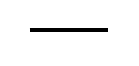
\begin{tikzpicture}[inner sep=0pt,baseline=(base)]%
        \draw[very thick, black,line width=1.5pt](0,0) -- (10mm,0); 
     %   \node[very thick, mark size=3pt,color=black] at (2.5mm,0){% 
      %      \pgfuseplotmark{diamond}%
       % };
        \node (base) at (0,-.5ex) {};
        \end{tikzpicture}%
    }
\usepackage{tikz}
\newcommand{\ImageWidth}{11cm}
\usetikzlibrary{shapes.multipart}
\usetikzlibrary{decorations.pathreplacing,positioning, arrows.meta}
\usetikzlibrary{shapes,arrows,chains}
\usetikzlibrary{shapes.geometric, arrows, calc, fit}
\usepackage{epigraph}
\setlength\epigraphwidth{8cm}
\setlength\epigraphrule{0pt}
\usepackage{multicol}
\usepackage{pdflscape}
\usepackage{fixmath}
\usepackage{bm}
\usepackage{bbm}
\usepackage{longtable}
\usepackage{multirow}
\usepackage{amsmath}
\usepackage{makecell}
\renewcommand\theadalign{cb}
\renewcommand\theadgape{\Gape[4pt]}
\renewcommand\cellgape{\Gape[4pt]}
\usepackage{amssymb,amsthm}
\usepackage{amsmath}
%\renewcommand{\thetable}{\Roman{table}}
%\addto\captionsenglish{\renewcommand*{\tablename}{TABLE}}
%\renewcommand{\thefigure}{\Roman{figure}}
%\addto\captionsenglish{\renewcommand*{\figurename}{FIGURE}}
\usepackage[labelfont=bf]{caption}
%\addto\captionsenglish{\renewcommand*{\figurename}{\textbf{Figure}}}
%\captionsetup[table]{labelformat=simple, labelsep=newline}
%\captionsetup[figure]{labelformat=simple, justification=centering, labelsep=newline}
\usepackage{scalerel}
\usepackage{tabularx}
\usepackage{booktabs}
\usepackage{amsmath}
\usepackage{plain}
\usepackage{mathptmx}
\usepackage{tcolorbox}
\makeatother
\usepackage{amsthm,amssymb}
\renewcommand{\qedsymbol}{\rule{0.7em}{0.7em}}
\renewcommand*{\thefootnote}{\fnsymbol{footnote}}
\renewcommand*{\thefootnote}{\arabic{footnote}}
\usepackage{graphicx}
\usepackage{mathtools}
\usepackage[hidelinks]{hyperref}
\hypersetup{
  colorlinks   = true, %Colours links instead of ugly boxes
  urlcolor     = orange, %Colour for external hyperlinks
  linkcolor    = orange, %Colour of internal links
  citecolor   = orange %Colour of citations
}
\tolerance 1414
\hbadness 1414
\emergencystretch 1.5em
\hfuzz 0.3pt
\widowpenalty = 10000
\clubpenalty=10000
\vfuzz \hfuzz
\raggedbottom
\date{\today}
%\author{Pedro Tremacoldi-Rossi}
\usepackage{array}
\usepackage[left=0.8in, right=0.8in, bottom=1in, top=1in]{geometry}
\usepackage{amsmath}
\usepackage{amssymb}
\DeclareMathOperator*{\argmin}{arg\,min}
\newcolumntype{P}[1]{>{\centering\arraybackslash}p{#1}}
\newcolumntype{M}[1]{>{\centering\arraybackslash}m{#1}}
\renewcommand{\vec}[1]{\mathbf{#1}}
\usepackage{tikz}
\usetikzlibrary{datavisualization}
\usetikzlibrary{patterns}
\usepackage{pgfplots}
\pgfplotsset{xtick style={draw=none}}
\pgfplotsset{every tick label/.append style={font=\footnotesize}}
\pgfplotsset{ every non boxed x axis/.append style={x axis line style=-} }
\pgfplotsset{ every non boxed y axis/.append style={y axis line style=-} }
\usepackage{etoolbox}
\usepgfplotslibrary{dateplot}
\pgfplotsset{compat=1.12}
\usepackage{filecontents}
\usepackage{pgfplotstable}

 \usepackage{subfig} % thiago addition
 \usepackage{ragged2e}
 \usepackage{lscape}


 \begin{filecontents*}{data.csv}
x,ineligible,control
%10	,	3.250506476	,	1.277502243
%20	,	5.563136085	,	2.372443406
%30	,	8.389761835	,	3.511001793
%40	,	9.258990109	,	5.207753188
%50	,	11.64759732	,	5.902718706
%60	,	13.37089925	,	6.104251096
%70	,	13.67403182	,	5.840018248
%80	,	14.08547988	,	5.468314891
%90	,	14.50673404	,	5.518457349
100	,	15.76401715	,	4.958697388
110	,	16.90239492	,	3.395942759
120	,	17.04532776	,	3.114551789
130	,	16.84917628	,	2.25291856
140	,	16.92707439	,	2.491117622
150	,	17.12842491	,	2.6828006
160	,	17.19395624	,	2.735237523
170	,	17.14847372	,	2.490334146
180	,	17.01422201	,	2.467982697
190	,	17.21713411	,	2.389993267
200	,	17.32566497	,	2.182484075
210	,	17.74371239	,	2.429502838
220	,	17.7774742	,	2.443941179
230	,	18.11954402	,	2.319133467
240	,	18.15209728	,	1.883755903
250	,	18.02253621	,	2.29799081
260	,	17.95281673	,	2.196441139
270	,	18.03753545	,	2.173787493
280	,	17.97485194	,	2.494688033
290	,	18.00257098	,	2.397850411
300	,	18.15438261	,	2.519457065
310	,	18.25551858	,	2.404375646
320	,	18.22033876	,	2.548635946
330	,	18.32730214	,	2.827430253
340	,	18.28274103	,	2.772094468
350	,	18.23640298	,	2.60989257
360	,	18.19887784	,	2.679968894
370	,	18.23889187	,	2.545737085
380	,	18.2524672	,	2.485689253
390	,	18.13448917	,	2.277273468
400	,	18.03065486	,	2.296423858
410	,	17.94146085	,	2.264346115
420	,	17.94913699	,	2.292316206
430	,	17.98559715	,	2.241390271
440	,	17.9868057	,	2.209010331
450	,	17.98979119	,	2.181342439
460	,	17.96811492	,	2.125704457
470	,	17.97756799	,	2.200190631
480	,	17.89654672	,	2.056534726
490	,	17.90308608	,	2.140444996
500	,	17.80451079	,	2.247613309
510	,	17.85333773	,	2.011227434
520	,	17.85866855	,	1.904663517
530	,	17.92625806	,	1.835191589
540	,	17.95916434	,	1.844615685
550	,	17.91574	,	1.733339721
560	,	17.95276855	,	1.705671828
570	,	17.96982597	,	1.812537943
580	,	17.93343759	,	1.998300081
590	,	17.91702034	,	2.068074207
600	,	17.96463873	,	2.133136285
610	,	17.99463131	,	2.045118363
620	,	17.99640825	,	1.975646435
630	,	18.04871727	,	1.924720501
640	,	18.02760938	,	1.83199053
650	,	18.04288986	,	1.855248572
660	,	18.09754421	,	1.762518602
670	,	18.08581761	,	1.771942698
680	,	18.03649407	,	1.716304716
690	,	18.10230664	,	1.683924776
700	,	18.19043566	,	1.651544835
710	,	18.21808292	,	1.656256883
720	,	18.19988873	,	1.781668992
730	,	18.08127053	,	1.712197063
740	,	18.1294573	,	1.679817123
750	,	18.14239246	,	1.684529171
760	,	18.10422715	,	1.754303297
770	,	18.09015522	,	1.717211309
780	,	18.09605442	,	1.763727393
790	,	18.06904733	,	1.852047514
800	,	18.09491765	,	2.000717664
810	,	18.11844265	,	2.065779742
820	,	18.08674492	,	2.112295826
830	,	18.08148589	,	2.093749832
840	,	18.06094638	,	2.061369892
850	,	18.05391042	,	1.987185916
860	,	17.99755091	,	2.010443958
870	,	18.00345011	,	1.936259981
880	,	18.01816221	,	1.824984017
890	,	18.05050011	,	1.797316125
900	,	18.01176641	,	1.811452269
910	,	18.03351448	,	1.7096004
920	,	18.07288834	,	1.714312448
930	,	18.04353593	,	1.603036484
940	,	18.05000351	,	1.626294526
950	,	18.1005356	,	1.556822598
960	,	18.13344189	,	1.603338682
970	,	18.14993093	,	1.60805073
980	,	18.2069306	,	1.520032807
990	,	18.24573608	,	1.469106873
1000	,	18.29100915	,	1.311617023
1010	,	18.24346255	,	1.13086913
1020	,	18.22526836	,	1.21918925
1030	,	18.30813835	,	1.18680931
1040	,	18.2829082	,	1.219491448
1050	,	18.28411675	,	1.052577501
1060	,	18.25476434	,	1.020197561
1070	,	18.32938982	,	1.168867712
1080	,	18.34879256	,	1.076137741
1090	,	18.34587885	,	1.020499759
1100	,	18.34296515	,	0.835039818
1110	,	18.30657677	,	0.76556789
1120	,	18.32363419	,	0.774991986
1130	,	18.33365565	,	0.802962076
1140	,	18.30664856	,	0.868024154
1150	,	18.33308726	,	0.812386172
1160	,	18.33720952	,	0.895994244
1170	,	18.33898646	,	0.93779828
1180	,	18.3407634	,	0.84506831
1190	,	18.35604388	,	0.826522316
1200	,	18.35369856	,	0.733792346
1210	,	18.36897904	,	0.859204454
1220	,	18.39307243	,	0.789732526
1230	,	18.40188533	,	0.794444574
1240	,	18.39954001	,	0.859506652
1250	,	18.38603646	,	0.8642187
1260	,	18.37665518	,	0.790034724
1270	,	18.38077743	,	0.855096802
1280	,	18.39840324	,	0.878354844
1290	,	18.38255437	,	0.841262856
1300	,	18.36023792	,	0.767078879
1310	,	18.3667055	,	0.767078879
1320	,	18.37551841	,	0.808882916
1330	,	18.38198599	,	0.771790927
1340	,	18.36848244	,	0.813594964
1350	,	18.3814176	,	0.776502975
1360	,	18.38553986	,	0.781215023
1370	,	18.39200744	,	0.841565054
1380	,	18.38966212	,	0.962265114
1390	,	18.3785039	,	0.925173126
1400	,	18.37381326	,	1.045873186
1410	,	18.37793551	,	0.990235204
1420	,	18.34446084	,	1.013493246
1430	,	18.3309573	,	1.115647312
1440	,	18.28397908	,	1.06000933
1450	,	18.24581377	,	0.96727936
1460	,	18.2299649	,	0.93489942
1470	,	18.22761958	,	0.860715443
1480	,	18.21646136	,	0.767985473
1490	,	18.24055474	,	0.698513545
1500	,	18.20416636	,	0.763575623
1510	,	18.09905171	,	0.745029629
1520	,	17.96046238	,	0.768287671
1530	,	17.86003837	,	0.768287671
1540	,	17.80602419	,	0.749741677
1550	,	17.64277309	,	0.731195683
1560	,	17.49771619	,	0.731195683
1570	,	17.4172633	,	0.772999719
1580	,	17.25870285	,	0.717361737
1590	,	17.13596239	,	0.717361737
1600	,	17.04435128	,	0.819515803
1610	,	16.97271129	,	0.763877821
1620	,	16.88991309	,	0.726785833
1630	,	16.7648273	,	0.708239839
1640	,	16.66205797	,	0.67114785
1650	,	16.62623798	,	0.652601856
1660	,	16.5011522	,	0.652601856
1670	,	16.42069931	,	0.652601856
1680	,	16.37372109	,	0.615509868
1690	,	16.28445531	,	0.559871886
1700	,	16.17052775	,	0.522779898
1710	,	16.07657132	,	0.504233904
1720	,	15.93151441	,	0.564583934
1730	,	15.8399033	,	0.564583934
1740	,	15.77707622	,	0.527491946
1750	,	15.70778155	,	0.569295982
1760	,	15.57388287	,	0.495112006
1770	,	15.50458821	,	0.476566012
1780	,	15.43763886	,	0.420928029
1790	,	15.27026551	,	0.402382035
1800	,	15.16749618	,	0.383836041
1810	,	15.12286328	,	0.383836041
1820	,	14.98192863	,	0.485990108
1830	,	14.91028865	,	0.546340138
1840	,	14.83864866	,	0.551052186
1850	,	14.77169932	,	0.551052186
1860	,	14.73353401	,	0.551052186
1870	,	14.66658467	,	0.551052186
1880	,	14.5884771	,	0.611402216
1890	,	14.55912469	,	0.592856222
1900	,	14.40290956	,	0.53721824
1910	,	14.3336149	,	0.518672246
1920	,	14.30660781	,	0.560476282
1930	,	14.25081669	,	0.583734324
1940	,	14.16801848	,	0.546642336
1950	,	14.04527802	,	0.588446372
1960	,	13.92019224	,	0.551354384
1970	,	13.72581179	,	0.477170407
1980	,	13.56725134	,	0.440078419
1990	,	13.364058	,	0.444790467
2000	,	13.16733223	,	0.407698479
2010	,	12.883686	,	0.393864533
2020	,	12.74978731	,	0.375318539
2030	,	12.6581762	,	0.380030587
2040	,	12.55775219	,	0.380030587
2050	,	12.49257979	,	0.324392605
2060	,	12.30288998	,	0.287300617
2070	,	12.23594064	,	0.287300617
2080	,	12.2224371	,	0.21311664
2090	,	12.14845179	,	0.194570646
2100	,	12.12379002	,	0.138932664
2110	,	12.07681181	,	0.101840676
2120	,	12.03864649	,	0.083294682
2130	,	11.97816473	,	0.0276567
2140	,	11.87774072	,	0.009110706
2150	,	11.79728783	,	-0.027981283
2160	,	11.6945185	,	-0.00472324
2170	,	11.65869851	,	-0.023269235
2180	,	11.55592917	,	-1.12E-05
2190	,	11.48663451	,	-1.12E-05
2200	,	11.42849807	,	0.02324685
2210	,	11.33688696	,	0.004700855
2220	,	11.2229594	,	-0.013845139
2230	,	11.15366474	,	-0.013845139
2240	,	11.07555717	,	0.027958898
2250	,	10.96162962	,	0.009412903
2260	,	10.93696785	,	-0.009133091
2270	,	10.83419851	,	-0.064771073
2280	,	10.74493272	,	-0.060059025
2290	,	10.69560919	,	-0.078605019
2300	,	10.6063434	,	-0.078605019
2310	,	10.54820696	,	-0.134243001
2320	,	10.49241584	,	-0.134243001
2330	,	10.4254665	,	-0.152788995
2340	,	10.31388426	,	-0.087726917
2350	,	10.25574782	,	-0.027376887
2360	,	10.16648203	,	-0.064468875
2370	,	10.14182026	,	-0.004118845
2380	,	10.0637127	,	0.037685191
2390	,	9.974446911	,	0.042397239
2400	,	9.860519353	,	0.023851245
2410	,	9.835857584	,	0.010017299
2420	,	9.713117125	,	-0.022362641
2430	,	9.677297132	,	-0.133638605
2440	,	9.527549582	,	-0.170730594
2450	,	9.42712557	,	-0.221656528
2460	,	9.337859781	,	-0.198398486
2470	,	9.203961098	,	-0.235490474
2480	,	9.09003354	,	-0.235490474
2490	,	8.96729308	,	-0.170428396
2500	,	8.734747322	,	-0.37443433
2510	,	8.654294435	,	-0.230476228
2520	,	8.629632666	,	-0.249022222
2530	,	8.551525101	,	-0.28611421
2540	,	8.551525101	,	-0.304660204
2550	,	8.526863332	,	-0.360298186
2560	,	8.49104334	,	-0.337040144
2570	,	8.446410446	,	-0.355586138
2580	,	8.412935775	,	-0.355586138
2590	,	8.36830288	,	-0.355586138
2600	,	8.334828209	,	-0.374132133
2610	,	8.290195315	,	-0.332328096
2620	,	8.267878868	,	-0.332328096
2630	,	8.243217099	,	-0.35087409
2640	,	8.220900652	,	-0.369420085
2650	,	8.207397107	,	-0.387966079
2660	,	8.151605989	,	-0.406512073
2670	,	8.095814871	,	-0.443604061
2680	,	8.051181976	,	-0.443604061
2690	,	8.017707305	,	-0.383254031
2700	,	8.006549082	,	-0.383254031
2710	,	7.993045537	,	-0.322904
2720	,	7.937254419	,	-0.322904
2730	,	7.914937971	,	-0.341449995
2740	,	7.901434426	,	-0.359995989
2750	,	7.867959755	,	-0.359995989
2760	,	7.834485085	,	-0.359995989
2770	,	7.756377519	,	-0.397087977
2780	,	7.745219296	,	-0.434179965
2790	,	7.700586401	,	-0.434179965
2800	,	7.700586401	,	-0.373829935
2810	,	7.678269954	,	-0.373829935
2820	,	7.66711173	,	-0.392375929
2830	,	7.653608185	,	-0.410921923
2840	,	7.608975291	,	-0.429467917
2850	,	7.564342396	,	-0.429467917
2860	,	7.542025949	,	-0.429467917
2870	,	7.508551278	,	-0.429467917
2880	,	7.486234831	,	-0.448013911
2890	,	7.441601937	,	-0.406209875
2900	,	7.419285489	,	-0.406209875
2910	,	7.396969042	,	-0.345859845
2920	,	7.318861477	,	-0.345859845
2930	,	7.305357932	,	-0.345859845
2940	,	7.236063269	,	-0.364405839
2950	,	7.157955703	,	-0.364405839
2960	,	7.14679748	,	-0.382951833
2970	,	7.122135711	,	-0.382951833
2980	,	7.055186369	,	-0.359693791
2990	,	6.954762357	,	-0.359693791
3000	,	6.905438819	,	-0.378239785
3010	,	6.838489478	,	-0.452423761
3020	,	6.791511262	,	-0.470969755
3030	,	6.797978842	,	-0.489515749
3040	,	6.764504171	,	-0.447711713
3050	,	6.706367732	,	-0.447711713
3060	,	6.70402241	,	-0.447711713
3070	,	6.681705963	,	-0.447711713
3080	,	6.648231292	,	-0.447711713
3090	,	6.603598398	,	-0.447711713
3100	,	6.590094853	,	-0.466257707
3110	,	6.576591308	,	-0.466257707
3120	,	6.565433084	,	-0.466257707
3130	,	6.520800189	,	-0.484803701
3140	,	6.509641966	,	-0.484803701
3150	,	6.498483742	,	-0.521895689
3160	,	6.476167295	,	-0.521895689
3170	,	6.442692624	,	-0.540441683
3180	,	6.431534401	,	-0.540441683
3190	,	6.420376177	,	-0.558987677
3200	,	6.384556185	,	-0.558987677
3210	,	6.393369087	,	-0.558987677
3220	,	6.346390871	,	-0.558987677
3230	,	6.324074424	,	-0.558987677
3240	,	6.321729102	,	-0.558987677
3250	,	6.321729102	,	-0.558987677
3260	,	6.321729102	,	-0.558987677
3270	,	6.299412655	,	-0.596079666
3280	,	6.288254431	,	-0.596079666
3290	,	6.25477976	,	-0.535729635
3300	,	6.243621537	,	-0.572821624
3310	,	6.22130509	,	-0.572821624
3320	,	6.176672195	,	-0.609913612
3330	,	6.154355748	,	-0.609913612
3340	,	6.132039301	,	-0.609913612
3350	,	6.109722853	,	-0.609913612
3360	,	6.09856463	,	-0.609913612
3370	,	6.087406406	,	-0.628459606
3380	,	6.087406406	,	-0.628459606
3390	,	6.053931735	,	-0.6470056
3400	,	6.038082869	,	-0.6470056
3410	,	6.038082869	,	-0.58665557
3420	,	6.038082869	,	-0.623747558
3430	,	6.015766421	,	-0.623747558
3440	,	5.993449974	,	-0.623747558
3450	,	5.991104653	,	-0.642293552
3460	,	5.991104653	,	-0.642293552
3470	,	5.991104653	,	-0.642293552
3480	,	5.979946429	,	-0.642293552
3490	,	5.966442884	,	-0.642293552
3500	,	5.95528466	,	-0.660839546
3510	,	5.944126437	,	-0.660839546
3520	,	5.910651766	,	-0.660839546
3530	,	5.910651766	,	-0.660839546
3540	,	5.899493542	,	-0.67938554
3550	,	5.866018871	,	-0.67938554
3560	,	5.854860648	,	-0.67938554
3570	,	5.86367355	,	-0.67938554
3580	,	5.852515326	,	-0.697931534
3590	,	5.827853558	,	-0.697931534
3600	,	5.794378887	,	-0.716477528
3610	,	5.792033565	,	-0.735023522
3620	,	5.758558894	,	-0.735023522
3630	,	5.736242447	,	-0.77211551
3640	,	5.736242447	,	-0.77211551
3650	,	5.713926	,	-0.77211551
3660	,	5.702767776	,	-0.77211551
3670	,	5.691609553	,	-0.77211551
3680	,	5.680451329	,	-0.77211551
3690	,	5.658134882	,	-0.77211551
3700	,	5.658134882	,	-0.77211551
3710	,	5.635818435	,	-0.77211551
3720	,	5.635818435	,	-0.77211551
3730	,	5.602343764	,	-0.730311474
3740	,	5.59118554	,	-0.730311474
3750	,	5.580027317	,	-0.730311474
3760	,	5.580027317	,	-0.730311474
3770	,	5.568869093	,	-0.748857468
3780	,	5.524236199	,	-0.767403462
3790	,	5.501919751	,	-0.767403462
3800	,	5.479603304	,	-0.785949456
3810	,	5.479603304	,	-0.80449545
3820	,	5.479603304	,	-0.80449545
3830	,	5.479603304	,	-0.80449545
3840	,	5.468445081	,	-0.80449545
3850	,	5.446128633	,	-0.841587439
3860	,	5.446128633	,	-0.860133433
3870	,	5.443783312	,	-0.860133433
3880	,	5.410308641	,	-0.860133433
3890	,	5.399150417	,	-0.860133433
3900	,	5.396805096	,	-0.860133433
3910	,	5.385646872	,	-0.860133433
3920	,	5.383301551	,	-0.860133433
3930	,	5.372143327	,	-0.860133433
3940	,	5.360985103	,	-0.860133433
3950	,	5.338668656	,	-0.860133433
3960	,	5.294035762	,	-0.860133433
3970	,	5.271719315	,	-0.878679427
3980	,	5.271719315	,	-0.897225421
3990	,	5.22708642	,	-0.897225421
4000	,	5.215928197	,	-0.897225421
4010	,	5.193611749	,	-0.915771415
4020	,	5.182453526	,	-0.915771415
4030	,	5.160137078	,	-0.915771415
4040	,	5.137820631	,	-0.915771415
4050	,	5.13547531	,	-0.915771415
4060	,	5.113158863	,	-0.934317409
4070	,	5.090842415	,	-0.934317409
4080	,	5.090842415	,	-0.934317409
4090	,	5.079684192	,	-0.934317409
4100	,	5.079684192	,	-0.934317409
4110	,	5.079684192	,	-0.934317409
4120	,	5.079684192	,	-0.934317409
4130	,	5.068525968	,	-0.934317409
4140	,	5.07733887	,	-0.952863403
4150	,	5.032705976	,	-0.971409397
4160	,	5.010389529	,	-0.971409397
4170	,	4.988073081	,	-0.971409397
4180	,	4.976914858	,	-0.971409397
4190	,	4.974569536	,	-0.989955391
4200	,	4.963411313	,	-0.929605361
4210	,	4.938749544	,	-0.929605361
4220	,	4.916433097	,	-0.929605361
4230	,	4.914087775	,	-0.929605361
4240	,	4.909397132	,	-0.929605361
4250	,	4.898238908	,	-0.929605361
4260	,	4.875922461	,	-0.924893313
4270	,	4.84244779	,	-0.943439307
4280	,	4.831289567	,	-0.943439307
4290	,	4.797814896	,	-0.943439307
4300	,	4.764340225	,	-0.943439307
4310	,	4.770807806	,	-0.961985301
4320	,	4.768462484	,	-0.961985301
4330	,	4.75730426	,	-0.980531295
4340	,	4.743800715	,	-0.980531295
4350	,	4.721484268	,	-0.999077289
4360	,	4.585240263	,	-0.975819247
4370	,	4.540607369	,	-0.994365241
4380	,	4.507132698	,	-0.994365241
4390	,	4.484816251	,	-1.012911235
4400	,	4.462499804	,	-1.012911235
4410	,	4.417866909	,	-1.012911235
4420	,	4.415521588	,	-1.050003223
4430	,	4.39320514	,	-1.050003223
4440	,	4.382046917	,	-1.050003223
4450	,	4.368543372	,	-1.050003223
4460	,	4.377356274	,	-1.050003223
4470	,	4.355039827	,	-1.050003223
4480	,	4.343881603	,	-1.050003223
4490	,	4.332723379	,	-1.050003223
4500	,	4.332723379	,	-1.050003223
4510	,	4.276932261	,	-1.050003223
4520	,	4.27458694	,	-1.050003223
4530	,	4.263428716	,	-1.050003223
4540	,	4.252270492	,	-1.050003223
4550	,	4.218795822	,	-1.068549218
4560	,	4.185321151	,	-1.068549218
4570	,	4.174162927	,	-1.068549218
4580	,	4.160659382	,	-1.068549218
4590	,	4.160659382	,	-1.068549218
4600	,	4.149501158	,	-1.068549218
4610	,	4.104868264	,	-1.087095212
4620	,	4.104868264	,	-1.087095212
4630	,	4.091364719	,	-1.087095212
4640	,	4.091364719	,	-1.087095212
4650	,	4.080206495	,	-1.087095212
4660	,	4.057890048	,	-1.087095212
4670	,	4.057890048	,	-1.087095212
4680	,	4.057890048	,	-1.087095212
4690	,	4.035573601	,	-1.087095212
4700	,	4.035573601	,	-1.026745181
4710	,	4.024415377	,	-1.026745181
4720	,	4.024415377	,	-1.026745181
4730	,	4.013257154	,	-1.045291175
4740	,	3.997408287	,	-1.045291175
4750	,	3.986250063	,	-1.045291175
4760	,	3.97509184	,	-1.045291175
4770	,	3.963933616	,	-1.045291175
4780	,	3.963933616	,	-1.045291175
4790	,	3.941617169	,	-1.045291175
4800	,	3.941617169	,	-1.045291175
4810	,	3.930458945	,	-1.045291175
4820	,	3.908142498	,	-1.045291175
4830	,	3.908142498	,	-1.045291175
4840	,	3.896984274	,	-1.045291175
4850	,	3.885826051	,	-1.06383717
4860	,	3.874667827	,	-1.06383717
4870	,	3.85235138	,	-1.06383717
4880	,	3.830034933	,	-1.06383717
4890	,	3.830034933	,	-1.06383717
4900	,	3.830034933	,	-1.06383717
4910	,	3.830034933	,	-1.06383717
4920	,	3.830034933	,	-1.06383717
4930	,	3.827689611	,	-1.082383164
4940	,	3.827689611	,	-1.082383164
4950	,	3.827689611	,	-1.100929158
4960	,	3.816531388	,	-1.100929158
4970	,	3.805373164	,	-1.100929158
4980	,	3.805373164	,	-1.100929158
4990	,	3.805373164	,	-1.100929158
5000	,	3.79421494	,	-1.15656714
\end{filecontents*}

\begin{document}
	\title{\LARGE \textsc{Amnesty and Land Grabbing in the Amazon}\thanks{We thank Thiago Alckmin, Tomas Etlin, Guilherme Vianna, Preach?, and Patricio Hernandez for outstanding research assistance.}}
	
	
	\author{ \ \ \ Jos{\'e} A. Scheinkman \\  \vspace{-0.5cm}  \small{ \ \ \  \textsc{Columbia University,}} \\ \vspace{-0.5cm} \small{ \ \ \  \textsc{Princeton University}} \\  \small{ \ \ \  \textsc{and NBER}} \and \  Pedro Tremacoldi-Rossi \\ \small{\textsc{Columbia University}}}
	\maketitle
    %\begin{center}
    %\textit{Preliminary and incomplete}
    %\end{center}
  %  \begin{center}
   % \textit{Preliminary and incomplete}
    %\end{center}
	\begin{abstract}
		\singlespacing
		\noindent 
		\PTR{This paper.}

 	\noindent \medskip{}
		
		
		\noindent \emph{Keywords:  }
		
	%	\noindent \emph{\bf JEL Classification: }  \emph{.}
	\end{abstract}
	\setcounter{page}{0}
\thispagestyle{empty}
	\noindent 

\clearpage

\section{Introduction}



%for every 2 hectares of forest kept in eligible properties, the unintended response induced in land-grabbers occupying ineligible areas resulted in 75 hectares of deforestation.
 

Brazil's 2012 forest code provided amnesty to illegal deforestation in the Amazon for  properties of less than...if deforestation occurred  before 2009. 

It was a contentious new law supported by \textit{ruralistas} (agribusiness) and opposed by a coalition of environmental groups and scientists.

“Land regularization restores citizenship to farmers, combats land grabbing, drastically reduces land
conflicts and violence, and contributes decisively to reducing deforestation” President Lula (2010)

“The policy may solve a practical, short-term problem, but it creates a negative incentive. The message is
that land invasion and deforestation will always be forgiven.” Paulo Barreto (Imazon, 2009)

Supporters argued that the new legislation would incorporate previously illegal properties into a legal framework, promote greater compliance over time, and encourage environmental restoration where feasible (cite). Critics, however, contended that granting amnesty for past illegal deforestation could set a dangerous precedent, potentially encouraging future land grabbing and unlawful clearing of forests (cite).

In this paper we examine empirically the ex-post validity of these opposing claims. If expectations were not affected, we could simply compare differences in the outcome around the law change-date between properties eligible for forgiveness to those that were ineligible. The possibility of a change in expectations requires a more careful treatment of ineligible areas, since land-grabbers may expect that  some ineligible areas  may soon benefit from another amnesty.

%For this reason we distinguish between three  types of ineligible areas:
%\begin{enumerate}
%\item Land designated to indigenous peoples, which are protected in the Brazilian constitution.
%\item Land designated as conservation areas.  
%\item Land outside federal areas. 
%\item Areas which are in eligible i.e. in non-designated federal land  but fail to qualify because of size and/or date of occupation. We will refer to these areas as policy induced controls.
%\end{enumerate}

\JS{ Pedro: Estamos usando estas 4 classes ou merging (1)  (2) e (3)? De todo modo é melhor inicialmente considerar as 4 classes  }
\PTR{Addressed!}


\begin{comment}
There are $i=1,...,N$ land parcels with evidence of occupation at given year $t$. We refer to these parcels as ``rural properties'' and detail in \textbf{Section X} how we identify them. We want to study both the ``direct'' effect of new eligibility rules for legal-ownership  on an outcome $y_i$, such as within-property deforestation rate --- and its indirect effects, including land-grabbing outside a property boundary 


\quad The potential effects of the forgiveness policy operate through two mechanisms. The first is the direct effect of the policy, i.e. the effect on an outcome, say deforestation rate, from laws that  forgave past illegal land occupation and established new property rights. Policy eligibility can be described as a mapping $z(g;w)$ where $g$ includes the policy parameters and $w$ property information such as area and beginning of occupation. In a basic setting, one could simply compare differences in the outcome around the policy between properties eligible for forgiveness to those whose characteristics $w$ made them ineligible according to $g$. More realistically, enacting a forgiveness policy is likely to affect expectations in ways that make this standard approach inadequate. 


\quad Think about deforestation rates. One of the goals of the forgiveness policy may be to decrease deforestation rates. But both existing and potential deforesters may expect another iteration of the forgiveness policy in the future. Moreover, across the board, individuals may perceive the policy as an overall signal of weaker environmental enforcement. As a consequence, even if a property is located in an area where future forgiveness is highly unlikely, e.g. due to illegally occupying an indigenous reservation --- it may engage in further illegal activity because it expects weaker enforcement. 
\end{comment}

%Consider a standard setting with two time periods, $t=1,2$
%Non-eligible properties in eligible areas, $g(1, 0)$, receive expectational spillovers; properties in never-eligible areas $g(0, 0)$ are the control group.
%$(T^*, G, Y, T)$ where $T^*$ is an expectation treatment, $G$ is the group status of being eligible for the policy, $Y$ is an outcome, e.g. deforestation rate, and $T$ is a noisy measure of $T*$. Assume there exists a potential outcome function $Y(T*, G)$ so that each property has four potential outcomes: $Y(0,0)$, $Y(1,0)$, $Y(0,1)$, and $Y(1,1)$. In addition, there is another potential outcome function $T(T*, G, Y)$.
\ 

\quad In many settings, Students not qualifying for debt forgiveness may borrow more in anticipation of future change in eligibility
%To recover the direct effect of forgiveness, we compare properties eligible to the policy to those located in illegally occupied areas that had already been designated by the government. Moreover, the forgiveness policy text explicitly states that those area would not be eligible for forgiveness, whose legal groundings relied on land whose use was ``yet to be designated'' by the federal government. Thus, not only properties in indigenous reservations or conservation areas 

\section{Introduction - DRY RUN}

\iffalse
\subsection{who are they}
\
\textbf{``pure'' control.} land parcels outside eligibility area (outside \textit{glebas federais})
\ 
\\ 
\textbf{policy-induced control.} land parcels on eligible area but that fail to qualify for policy eligibility criteria
\ 
\\ 
\textbf{treatment-eligible.} land parcels that qualify for policy eligibility criteria.
\ 
\\ 
\textbf{treated.} land-grabbers of eligible parcels who applied for title program
\ 
\\ 
\textbf{already treated.} land parcels already titled, inside or outside eligibility area

\subsection{how to measure them}
\

\quad we observe \textbf{already treated} parcels directly from data (SNCI). we also observe \textbf{treated} parcels from the data, through a complicated linkage process we implement across multiple government data sources. this process involves some measurement error, both because we do not successfully geo-locate all program applicants and because the program applicant list may not be comprehensible. the other groups have to be constructed following another approach.
\ 

\quad based on CAR locations, we delimit land parcels which reasonably were valid at the time of entry in that registry. because CAR offers no direct legal coverage, property limits can be different than in reality. this includes the possibility that an area is registered without any occupancy or that overlays other areas already registered or that are owned by unrelated individuals. with CAR parcels as the geography of analysis, we use satellite imagery created by MapBiomas. they assign land coverage including around 40 different categories to 30$\times$30 meter imagery pixels captured by the landsat satellite. 
\ 

\quad we construct a ``legacy'' forest stock, which is made up by pixels with natural cover both in 1985 and 1986 --- the two first years data are available. then, we track each of the 5 billion pixels in the Amazon biome every year to check whether the land coverage in a pixel transitions from natural to anthropic --- which we define as an ultra-localized measure of deforestation. for a given CAR parcel, we can therefore track its entirety land cover back to 1985 and determine i) when occupation first began and ii) the size of that occupation.
\ 

\quad determining when occupation begins is necessary because the first policy eligibility criteria determines that only public land grabbed up to 2004 would be accepted. so our first assignment rule is simple: if an area has no evidence of human activity (which ranges from structure construction, simply taking down forest, or starting to grow soybeans) prior to 2005, that parcel is a \textbf{policy-induced control}. of course, if nobody \textit{ever} occupies that parcel, it would be an irrelevant control unit. here we exploit the 5-year gap between the eligibility criteria and policy announcement so that we only consider parcels with deforestation starting anytime during 2005-2009. similarly, \textbf{pure control} properties are those with human occupation anytime up to 2009 and located outside the public forests allocated for the amnesty program.
\

\quad how about parcels with evidence of human use prior to 2005? the other eligibility criteria determines that only individual land parcels no larger than 1,500 hectares (5.8 miles$^2$) would qualify. by ``individual'', the policy meant that a single individual could only apply in her own name (not under a corporation, for example) to have one parcel considered to be titled. this creates an interesting measurement problem for the econometricians (us). who is eligible and who is not?
\
\textit{incorrectly-assigned controls.} suppose a CAR in eligible public land with occupation in 2001 has an area of 2,000 hectares, which makes it look like a \textbf{policy-induced control}. but because individuals have an incentive to submit larger CAR areas than those they actually occupy (to later make ownership claims over the larger area), it may well be at the time of the policy eligibility this farmer would have qualified with the area criteria. note this is incentive-equivalent to the farmer occupying 2,000 hectares but submitting the largest qualifying land area and continuing to occupy the remaining area. however, these two cases leave different imagery footprints.

suppose a CAR with occupation in 2001 has an area of 150 hectares, which makes it look like a \textbf{treatment-eligible} parcel. but adjacent to this CAR, there are other CAR

\begin{itemize}
    \item \textbf{CAR:} land parcel \textit{claim}
    \item \textbf{SNCI, SIGEF, CAFIR:} land parcel title-ish
\end{itemize}

suppose a farmer occupied an area 10 times the size of that allowed for policy-eligibility, which in theory makes her look like a \textbf{policy-induced control}. but she knows only 1/10 of her parcel qualifies, so this is the dimension she would submit to the policy office. but what would she do in CAR? since this is our method of pinpointing eligible 
\fi 
 

\clearpage

\section{Setting and Data}

This section describes the main policy setting we explore --- a series of amnesties granted to land-grabbers illegally occupying public land in the Amazon --- as well as our main data sources and variable construction. We combine data from dozens of sources in the paper, from public records to satellite images. More details on those are available in the \appendixref{1}.

\subsection{Land Use in the Amazon}
\ 

\quad The Brazilian Amazon covers an area of 420 million hectares, approximately half the size of the continental US. Almost all forest area is under federal or state jurisdiction, with land broadly divided into two groups: areas under special protection (e.g., indigenous reservations, national parks, biological reserves) and undesignated lands. Undesignated areas are public forests waiting for an official use destination, comprising a massive area of almost 60 million hectares and storing the equivalent of one year of total global carbon emissions. Occupation of undesignated areas is illegal and, as a consequence, any deforestation in those areas is also illegal. 
\ 

\quad The vast amounts of Amazon forest without official designation have long been a concern for the Brazilian government and environmentalists. Land grab in those areas is rampant, and deforestation rates tend to be much higher than in the rest of the Amazon. Based on the satellite data we introduce below and conversations with environmental watchdogs, we estimate well over a hundred thousand individuals illegally occupying land in undesignated areas with evidence of ongoing or recent deforestation. Although some of these squatters have occupied small plots of land to produce agricultural produce, the majority of deforested and not abandoned land in undesignated areas is used for cattle farming, with many individuals claiming ownership over more than one parcel.  
\ 

\quad To address the complex land use situation in the Amazon, the Brazilian government has combined a menu of policies including direct repression and more accommodating strategies. On the repressive side, the country has invested in real-time monitoring systems and increased the scope and weight of sanctions against illegal deforestation and other environmental violations. However, enforcement effectiveness is heavily based on obligations tied to property rights of rural properties, such that illegally occupied areas make enforcement more difficult.\footnote{For instance, Brazil's advanced deforestation warnings system is more effective if affected areas can be linked to specific individuals, and there are strict deforestation ceilings and other land-use rules that legal rural properties need to comply to maintain their land title.} Despite a robust monitoring system, enforcement is costly and its intensity varies strongly depending on different administrations' degrees of commitment to preservation (e.g., \cite{10.1257/app.20200196} and \citet{burgess2023national}.). In practice, expropriation of squatters is rare and it is very difficult to prevent their return or dislocation to clear forest in another public area. 
%and to meet the increasingly important goal of environmental preservation
%, the Brazilian government has adopted a mix of accommodating and repressive policies, with environmental preservation increasingly becoming the policy main goal. 
%The environmental agenda in the country is heavily based on obligations tied to property rights of rural properties, such that illegally occupied areas make enforcement more difficult.\footnote{For instance, Brazil's advanced deforestation warnings system is more effective if affected areas can be linked to specific individuals, and there are strict deforestation ceilings and other land-use rules that legal rural properties need to comply to maintain their land title.} Despite a robust monitoring system, enforcement is costly and its intensity varies strongly depending on different administrations' degrees of commitment to preservation (\textbf{see, e.g., }). In practice, expropriation of squatters is rare and it is very difficult to prevent their return or dislocation to clear forest in another public area. 
\ 

\quad In recognition of these challenges, policymakers started to acknowledge the possibility of ``accommodating'' certain individuals occupying public land, granting them legal ownership of their rural parcels with the ultimate goal of environmental preservation. With legal ownership, rural land owners must comply with strict land use and deforestation thresholds and environmental sanctions are more easily implemented. In this context, the Brazilian government implemented an amnesty for certain land-grabbers in 2009. In 2017, a new amnesty was introduced with even more lenient qualifying criteria. 
%legal rural properties need to comply with strict deforestation ceilings and other land-use rules to ensure preservation.  
%Because undesignated areas can potentially be allocated to land reform policies or certain private titling (e.g., sustainable farming) instead of receiving specially protected status, squatters see these areas 


\subsection{Land-Grabbing Amnesty in the Amazon}

\subsubsection{The 2009 Land-Grabbing Amnesty}
\ 

\quad \textbf{Context---} In 2009, a reform named \textit{Programa Terra Legal} offered amnesty to a certain group of land-grabbers in federal undesignated land. The goal of the program was to target ``long-established'' squatters, allowing only parcels smaller than 1,500 hectares and that had been occupied at least since 2004 to be eligible for amnesty. The policy size threshold was much larger than most regional definitions of a small property used by the Brazilian government (anywhere from 20 to 200 hectares). For comparison, the average farm size in the US is under 200 hectares. Moreover, most land titles were given for free or at virtually no cost to squatters. Ownership titles also imposed no or very loosely defined constraints on future sales. Finally, no additional environmental rules or targets were tied to the titles other than the standard requirements applicable to any landowner in the Amazon.
\ 

\quad The amnesty was first introduced through Provisional Measure 458, signed by President Lula in February 2009, and was enacted into law by Congress in June 2009 (Law 11952). The Land-Grabbing Amnesty was contentious, supported by the Lula Administration and \textit{ruralistas} (agribusiness), while opposed by a coalition of environmental groups and scientists. The following contemporaneous quotes provide a summary of the opposing viewpoints between the two groups: 
\begin{quote}
  ``\textit{Land regularization restores citizenship to farmers, combats land grabbing, drastically reduces land
conflicts and violence, and contributes decisively to reducing deforestation.}'' --- President Lula (2010) 
\end{quote}
\begin{quote}
``\textit{The policy may solve a practical, short-term problem, but it creates a negative incentive. The message
is that land invasion and deforestation will always be forgiven.}'' \quad\quad \quad \quad \quad \quad  --- Paulo Barreto (Imazon, 2009)
\end{quote}
\ 

\quad Clearly, advocates for the Amnesty focused on the cost and limited success of previous policies that attempted to resolve land conflict in the Amazon and curb illegal deforestation. In opposition, environmentalists were concerned that the policy induced moral hazard, potentially leading to more land-grabbing and deforestation under the expectation of another amnesty in the future. The potential intertemporal effect of this policy is a key feature we explore in the paper. 
\ 

\quad \textbf{Policy roll-out and implementation---} The program implementation was slow and riddled with technical and logistical problems. Despite a large number of requests for amnesty eligibility (see \figref{applications}), only a small number of titles were given in the program's first year and claims took on average 3 years to be processed. Several of these setbacks involved an initial step in which the property boundaries submitted by applicants had to be verified and audited, as well as the need to establish occupation history and its compliance with the eligibility criteria. Many requests from different squatters included proposed property lines that overlapped, further requiring spatial conflict resolution by the government officials working on the program's roll-out. 
\ 

\quad Because program participation is endogenous, which land-grabbers are ultimately granted amnesty matter for the direct effects of the policy. This is determined by which eligible squatters decide to apply and receive forgiveness. Squatters with lower deforestation propensity may be more likely to apply, as those whose occupied areas have already been deforested more aggressively may see compliance costs as too high. This would select land-grabbers who would already deforest less absent the Amnesty, potentially reducing the positive effects expected by the Brazilian government. Similarly, property rights can raise the incentives to extract surplus through costly investment (i.e., deforesting) as uncertainty over who captures gains from land use decreases. This suggests the possibility that treatment effects from Amnesty may even increase deforestation if high-uncertainty squatters are more likely to apply.%\footnote{Conditional on the set of applicants, the policy roll-out may also systematically affect those being benefited by the Amnesty. For instance, if claims from more recent and larger occupiers are more easily audited, the resulting sample of those being benefited by the Amnesty may differ from the initial group the Brazilian government claimed to target correlates with... or targets certain characteristics, those receiving the benefic may differ from the unofficial policy goals (older, \textbf{small settlers)}. }
%It is not immediately clear whether legalization would reduce deforestation. On the one hand, property ownership increases the cost of illegal deforestation due to better enforcement, on the other, it also raises incentives to extract surplus as uncertainty over ownership from land gains decreases. Deforesting is costly and property rights could indeed increase forest removal. If the marginal squatter sees the policy The marginal squatter targeted during the design of the Amnesty may differ from the average applicant who sees the benefits from legalization as anticipated by the government may differ from the average applicant, for instance if individuals who see their remaining land surplus almost \textbf{depleted} . Finally, conditional on who applies for amnesty, if the program rollout is systematically slow or targets certain characteristics, those receiving the benefic may differ from the unofficial policy goals (older, small settlers).
\

\quad To shed some light into Amnesty take-up, \tabref{25} shows application and titling rates for land-grabbers eligible to apply for the 2009 Amnesty. Application rates have a lower bound of approximately 10\%, while until the program was into effect without any modifications (2016), 42\% of squatters with property boundaries audited were given ownership titles.\footnote{We can only match Amnesty requests to our eligible property data based on geography entries of properties that had their limits surveyed by the government. } Columns (1) and (2) analyze how various property characteristics predict take-up. While squatters occupying the land longer did not seem to be more likely to apply for amnesty, those in smaller areas were far more likely to apply. Since the program had as a goal to curb deforestation through ownership, we also check whether the share of deforested area as of 2008 predicts applications. 
\ 

\quad We find a concave pattern between pre-existing deforested rate and amnesty applications. Coefficient estimates suggest that higher deforestation rates predict a higher probability of amnesty requests until a deforested share of $\widehat{0.047}/[-2(\widehat{-0.052})]\approx45\%$, after which more deforestation is associated with lower application rates. Because these estimates are conditional on history of occupation, they are consistent with the following interpretation. For land-grabbers who invaded forest areas in the same year, those with larger investments may see property rights as a way to guarantee private returns on deforestation, making them more likely to apply for amnesty. But those who deforested at higher rates in the same period appear to weigh the costs from legalization more heavily, becoming less likely to apply.
%This response is consistent with squatters initially seeing property rights as a way to guarantee ownership from returns on deforestation, but then being crowded-out when  
\ 

\quad Columns (3) and (4) in \tabref{25} show conditional amnesty granted to applicants (which amounts to about 42\% of requests that were audited by the government). Overall, areas with a longer history of occupation (going back to 1989) are less likely to receive amnesty, with a nonlinear response where those with more recent occupation become more likely to be titled. There is also some evidence that amnesty rates for properties smaller than 100 hectares had higher success rates. We see these descriptive patterns as more likely to be picking-up inefficiencies during the roll-out process than a preference by policymakers for those attributes.

\subsubsection{The 2017 Land-Grabbing Amnesty}
\ 

\quad \textbf{Context---} In 2017, a new Amnesty was passed into law (converted from Provisional Measure 759) by the Temer Administration. Law 13465, signed in July, expanded amnesty eligibility for land-grabbers in the Amazon: invasions until 2011 and with areas up to 2,500 hectares were allowed to qualify for amnesty under the same terms of the existing \textit{Programa Terra Legal} from 2009. The property threshold size of 2,500 was seen as excessively large by critics --- approximately only 1\% of registered farms in Brazil and US, for reference --- which influenced the law's informal name of ``Land-Grabbing Act''. The updated occupation criteria also made land-grabbing occurring after the first Amnesty, and potentially a response to it, eligible for forgiveness in the new law.
\

\quad \textbf{Implementation and aftermath---} Certain aspects of the 2017 Land-Grabbing Amnesty were challenged in court, which nonetheless remained valid. As early as 2019 a new, third wave of amnesty was proposed by the Bolsonaro Administration, eliminating occupation tenure and area requirements altogether. This would effectively grant the possibility of amnesty to any land-grabber in undesignated public areas in the Amazon. Provisional Measure 910 expired without being enacted into law by Congress, leaving the 2017 eligibility cutoffs into effect. 


\subsection{Measuring Deforestation in the Amazon}
\

\quad Tracking deforestation in the Amazon is crucial to study the consequences of land-grabbing amnesties and to determine the patterns of human occupation in an area. We use high-resolution maps of land cover from \textit{MapBiomas} developed based on Landsat 30$\times$30-meter images. The Amazon biome is covered by several billion pixels of this scale, each being assigned a specific color code associated with a use cover (e.g., soybeans crop, pasture, native forest, human-built structures).\footnote{Because our data spans several decades, different versions of Landsat were operational and therefore contributed with images to the classification scheme used by \textit{MapBiomas}. More details on the classification methodology can be found at \href{https://brasil.mapbiomas.org/wp-content/uploads/sites/4/2025/08/Amazon-Appendix-ATBD-Collection-10-v2.pdf}{https://brasil.mapbiomas.org/wp-content/uploads/sites/4/2025/08/Amazon-Appendix-ATBD-Collection-10-v2.pdf}.} Thus, changes in pixel classifications over time identify changes in land cover.
\ 

\quad \textbf{Measuring land cover---} We construct a legacy forest stock (``as is'') corresponding to all pixels in the satellite imagery occupied by forest cover in 1985 and 1986, the first years with available satellite data. Panel (a) in \figref{1} shows the legacy forest in the Amazon biome. Based on this initial forest stock, we track what happens to the cover in each legacy forest pixel over time. If a forest pixel becomes covered with patterns consistent with human action, we denote that pixel as deforested. Once a pixel is assigned to deforested, it can remain as that or become reforested. We classify an area as reforested if it stays deforested for at least two consecutive years and then is covered by forest for at least three years. This is done to avoid hyper-granular noise at the pixel level. 
\ 

\quad Panels (b) through (d) in \figref{1} show the evolution of deforestation in the Amazon. By 2020, around 13\% of the forest existing in 1985-1986 had been deforested, an equivalent of 52 million hectares (more than the area of California). A small area equivalent to 8 million hectares has been reforested, either by human action or by vegetation growth following abandonment. 
\ 

\quad This satellite imagery plays two important roles in the paper. First, it allows us to track deforestation at a very granular level and therefore quantify the environmental consequences of the Brazilian government's amnesty agenda. Second, it also enables us to directly establish human occupation of a particular area.
\ 

\quad \textbf{Rural parcels---} Brazil has a centralized database attempting to organize records of rural parcels named Rural Environmental Property Registry (CAR). Rural property owners are required to submit information on their rural parcel, including several indicators meant to comply with environmental legislation and property boundaries to obtain a CAR code. The database is public and can be used by anyone to verify the status of a CAR code. The information submitted is self-reported and until Brazilian authorities verify the registration, the CAR code appears under the status ``pending''. However, because only an insignificant portion of submitted registrations is audited, effectively all parcels have pending CAR codes, which means legally and illegally occupied areas are indistinguishable in the database. This has created a loophole exploited by squatters, who submit registrations and obtain a (pending) CAR code, then use it informally as ``proof'' of occupation, especially for land transactions. 
\ 

\quad The CAR database therefore contains claimed property boundaries of legally and illegally occupied areas. While the nature of the data generating process is useful to us, because boundaries are self-reported, a large number of claimed property lines overlap. To avoid double-counting and other mechanical distortions, we develop a complex spatial resolution algorithm, described in \appendixref{2}. Though implied magnitudes change, all our results carry if we used property boundaries without any adjustment (see \sectionref{9}).
\ 

\quad In different parts of our analysis, we also use other sources containing property boundaries that have been audited or verified in different ways by Brazilian authorities. Those are described in detail in \appendixref{1}.
\ 

\quad \textbf{Establishing human occupation---} Land ownership claims in Brazil are mainly established through the idea of ``ownership by use'', where the most common strategy is to deforest portions of the land. This directly signals occupation to other potential land-grabbers and even fines received due to illegal deforestation are used in future petitions for legalization, as environmental sanctions identify the squatter in the area.\footnote{Even fencing, which is costly and without proper monitoring can be easily cut down or altered, requires forest cleaning prior to installation.} Consequently, satellite evidence of deforestation in a particular area indicates human occupation, while a property claim in a forest area without any associated identifiable deforestation points to a CAR record that should be discarded. 
\ 

\quad Since it is not possible to perfectly observe the identity of squatters, we rely on a measure of deforestation to establish human occupation. Specifically, the first year when the share of deforested area in a rural parcel reaches 10\% is assigned as the beginning of human occupation. We use 10\% since for very small areas a lower share could be affected by noise in satellite readings, though marginally changing our threshold has little effect on our point estimates. 
\

\quad \figref{human} shows an example of the evolution of human occupation within a rural property of about 2,000 hectares. We track pixel-by-pixel the 24,000 satellite readings that span the property. In 2002, approximately 26\% of the property was deforested, which meets our threshold to establish human occupation of 10\%. By 2004, 38\% of the property area had been deforested. By repeating the same process for each one of the hundreds of thousands of rural parcels in our data, we are able to measure eligibility for the amnesty policies and most of our outcomes.
%\subsection{Data Sources and Patterns}

\section{The Consequences of the First Amnesty} \label{sec:3}

\PTR{intro paragraph}

\subsection{Empirical Design}

\ 

\quad Conditional on occupying land in a target area, the 2009 Land-Grabbing Amnesty sharply defines eligibility based on two conditions: having started the illegal occupation up to 2004 and having occupied no more than 1,500 hectares. This would suggest a straightforward difference-in-differences design where we would compare eligible squatters to those ineligible in target areas to estimate treatment effects of policy eligibility.
\ 

\quad This difference-in-differences design, however, assumes that squatters who did not qualify for forgiveness provide a good counterfactual to those eligible. In practice, this rules out expectational effects, since land-grabbers assigned to the control group should behave as if the policy was absent.\footnote{Though not commonly discussed, the importance of expectational effects to proper identification of causal estimands is not exclusive to our setting. While many difference-in-differences implementations could credibly claim that the intervention was perceived as one-off, in principle any policy stipulating eligibility may generate anticipation of changes to these criteria at a future date. In cases of intertemporal changes in hazard of another intervention, like ours, it is crucial to identify a group for which under no set of conjectures eligibility status may likely change at a future date.} Beyond proper empirical design considerations, any response from this untargeted group could be interpreted as unintended consequences from a policy design perspective and drastically affect net effects of the Amnesty. For example, if ineligible squatters interpret the 2009 policy as a signal of future forgiveness, they could respond by invading more land in target areas.
%additional forgiveness coming down the pipe, they could increase land-grabbing and deforestation in target areas, possibly resulting in vastly different net effects were just responses of eligible land-grabbers being measured. 
\ 

\textbf{Setup---} To jointly address the design issue above and study the response of ineligible squatters, we set up our empirical design in the following way. First, we use an appropriate control group of land-grabbers for which any forgiveness expectation is always non-existent and remains unchanged with the 2009 policy. We select land-grabbers in indigenous reservations and conservation areas, both federal land whose status is strictly regulated by law.\footnote{The Brazilian Constitution prevents the introduction of any bill allowing the occupation of reservations by non-indigenous people (Article 231). Conservation units (e.g., national parks, biological reserves, ecological stations) are ``specially protected territorial areas'' whose suppression for private occupation would require the establishment of a complicated and overarching legal framework by Congress (Article 225). Besides the constitutional provision, a robust set of laws (e.g. Law 9985/2000) mandates expropriation of ``private enclaves'' from conservation units and also establishes that boundary reductions must each be made by a stand-alone, specific law. Consistent with this structure, land-use programs like the 2009 Land-Grabbing Amnesty have explicitly excluded these categories (Article 4 of the bill), leaving invaders with no reasonable path toward legalization.} We refer to these group of land-squatters as \textit{never-eligible} as they, in approximation, would never qualify to receive a title for the land they invaded. 
\ 

\quad Second, we consider a more general potential outcome function $Y_i(D_i^{\text{direct}}, D_i^{\text{expectations}})$, where a rural parcel $i$ (or a ``property'' without a legal ownership title) with treatment assignment status receives one of the two treatments as follows. \textit{Eligible} properties are exposed to the Amnesty direct treatment $D_i^\text{direct}$ and satisfy the policy eligibility criteria:
\begin{equation}
\underbrace{\mathbb{1}\{i \in \text{target area} \}}_{\text{assignment}}\times\underbrace{\mathbb{1}\{\text{occupied}(i)\leq 2004 \}\times\mathbb{1}\{\text{area}(i)\leq 1500 \}}_{\text{eligibility}} \label{eq:8}
\end{equation}
while \textit{ineligible} properties are those in target areas exposed to an expectation treatment $D_i^\text{expectations}$ despite having invaded land after 2004, more area than 1,500 hectares, or both.
%In canonical difference-in-differences designs, . This would imply that squatters ineligible for amnesty should not change their behavior because of the policy (or be indirectly affected through the treatment on eligible units, for example due to spatial spillovers). This is equivalent to completely shutting off an effect on expectations. Thus, if 
%If expectations were not affected, we could simply compare differences in the outcome around the law change-date between properties eligible for forgiveness to those that were ineligible. The possibility of a change in expectations requires a more careful treatment of ineligible areas, since land-grabbers may expect that some ineligible areas may soon benefit from another amnesty.Consider $K=2$ treatments in $D$ so that the potential outcome function $Y$ is given by $Y_i(D_i^{\text{\textbf{direct}}}, D_i^{\text{\textbf{expectations}}})$. 
\ 

\textbf{Characteristics of eligible, ineligible, and never-eligible land-grabbers---} \tabref{1} shows a selected number of summary statistics for the two treated groups (eligible and ineligible properties) and the control group (never-eligible) we use to quantify the impact of the 2009 Amnesty. There are considerably more eligible properties, which are smaller than ineligible and also those never eligible. Eligible properties also tend to have higher shares of deforested area, adding up to 5.1 million hectares of deforested area in 2008. This is 24\% more deforested area than that in ineligible properties and more than double of those in never-eligible parcels.
\ 

\quad The first suggestive evidence of a strong response from ineligible land-grabbers around the policy comes from changes in deforestation. \tabref{1} shows that the deforested area in those properties not eligible for forgiveness increases by over 15\% compared to a 11 percent-increase in the control areas. Between 2014 and 2009, an area larger than the US state of Delaware was deforested just in roughly 15,000 ineligible properties. Eligible properties display a much slower increase in deforested area, of about 6\% or around 200 thousand hectares.
\ 

\textbf{Main empirical model---} Our main empirical design therefore compares in two separate regressions eligible and ineligible properties to never-eligible properties: 
\begin{equation}
 y_{it}   = \beta x_i\times\mathbb{1}\{t\geq 2009\}+\upsilon_i+\upsilon_t+\varepsilon_{it} \label{eq:1}
\end{equation}
where $x_i$ is an eligibility indicator equal to one if rural parcel $i$ satisfies the direct treatment assignment in \eqref{eq:8}. \eqreffmt{1} also includes parcel fixed effects, which control for unobservable heterogeneity across properties --- e.g., differences in agricultural productivity or proximity to transportation routes --- and year effects to absorb common shocks over time. In alternative specifications we use year-by-geography $\upsilon_t\times\upsilon_{g(i)}$ interactions (time effects interacted with state or municipality dummies). These capture time-varying characteristics at a local geographic area which control for differential changes in environmental enforcement, weather shocks, or local labor market trends. We cluster standard errors at the state level and use the data period of 2005 to 2014. %This period experienced relatively stable changes in aggregate deforestation rates in the Amazon
%\begin{equation*}
%\underbrace{\mathbb{1}\{i \in \text{target area} \}}_{\text{assignment}}\times\underbrace{\mathbb{1}\{\text{occupied}(i)\leq 2004 \}\times\mathbb{1}\{\text{area}(i)\leq 1500 \}}_{\text{eligibility}}   
%\end{equation*}

\subsection{Impacts on Deforestation}
\ 

\quad We start our analysis of the consequences of the 2009 Land-Grabbing Amnesty on deforestation rates in eligible and ineligible properties. 
\

\quad \textbf{Eligibility effects---} \tabref{2} shows in columns (1) through (3) estimates on deforestation rates ($\text{deforested area}_t/\text{total area}_t$) for rural properties eligible to apply for the amnesty. Results show that program eligibility reduces deforestation rates by approximately 2\%, or an estimated $\widehat{\beta}$ of 1 percentage point for an average deforestation rate of 58\% in eligible properties before 2009. Panel (a) in \figref{3} plots event-study style estimates of the baseline model which show indistinguishable pre-trends in deforestation between eligible and control properties and a relative steady decline in the eligible group following the Amnesty law. 
\ 

\quad \textbf{Expectation effects---} In columns (4)--(6) of \tabref{2}, we show treatment effects for properties ineligible for the first land-grabbing amnesty. Because squatters in these properties were not allowed the treatment intended by the law --- legalization eligibility --- any measured causal response could be interpreted as ``unintended''. This response could align with the stated goals of the policy, resulting in a decrease in deforestation as a positive spillover, for example, or counteract the effects from targeted squatters. Our results support the second conjecture, revealing a striking response: deforestation rates increase by over 30\%, an effect one order of magnitude larger than the decrease in deforestation in eligible properties. 
\ 

\quad \textbf{Net effects on deforestation---} Using the reduced-form estimates above, we can compute the approximate average net effect of the first land-grabbing amnesty on deforestation in the Amazon. At the baseline, the 2.4\% decrease in deforestation translates to a ``counterfactual'' deforestation rate 34\% lower in eligible properties as a result of the amnesty.\footnote{The eligible property average deforestation rate increased from 58.4\% to 62.5\%, a 7\% increase. Extrapolating, it would've been 9.4\%, or 34\% higher.} In terms of forest cover, the average property avoided deforesting about 2 hectares: 
\begin{equation*}
    \underbrace{-1.4}_{\widehat{\beta} \text{ (p.p.)}}
    \times
    \underbrace{58.4}_{\shortstack{\scriptsize\text{pre-2009} \\ \scriptsize\text{deforestation rate (\%)}}}
    \times
    \underbrace{69.03}_{\shortstack{\scriptsize\text{pre-2009} \\ \scriptsize\text{deforested area (ha)}}}\approx2\text{ ha}
\end{equation*}
\ 

\quad We can then project the figure above to account for the total change in forest. Based on the numbers in \tabref{1}, the total deforested area in eligible properties changed from 5.1 million hectares in 2008 to 5.27 million ha in 2014. This means that about 54,000 hectares of forest were kept in eligible properties as a result of the policy. 
\ 

\quad We can perform a similar exercise for ineligible properties, where amnesty induced a large increase in deforestation. Because ineligible areas tend to be larger than eligible properties, this difference in treatment effects amplifies to a 75 hectare ``unintended'' increase in deforestation compared to the 2 hectare decrease for the average eligible squatter: 
\begin{equation*}
    \underbrace{4.2}_{\widehat{\beta} \text{ (p.p.)}}
    \times
    \underbrace{11.4}_{\shortstack{\scriptsize\text{pre-2009} \\ \scriptsize\text{deforestation rate (\%)}}}
    \times
    \underbrace{204.3}_{\shortstack{\scriptsize\text{pre-2009} \\ \scriptsize\text{deforested area (ha)}}}\approx75\text{ ha}
\end{equation*}
\

\quad  From the data, the deforested area increased to 4.66 million hectares in 2014 from 4.1 million ha in 2008. Since the average deforestation rate increased to 21.4\% in the period, this implies that 42\% of the observed deforestation in public land not targeted by the amnesty is attributable to expectation effects, an equivalent of 227,000 hectares of forest being cut. Taken together, intended and unintended responses to the amnesty resulted in a net removal of forest of 173 thousand hectares. This is a substantial number: on average, about 1\% of the existing forest stock in non-designated areas is taken down every year, roughly 117 thousand hectares. The net effect of the amnesty thus amounts to almost 1.5 years of additional deforestation in a short timespan. 
\ 

\quad \textbf{Equivalence in released carbon---}The additional forest removed as a consequence of the 2009 Land-Grabbing Amnesty released a non-trivial amount of CO$_2$ into the atmosphere. Using the approximate 500 tons of CO$_2$ that the average hectare in the Amazon stores (\citet{scheinkman2024carbon}), the 173 thousand hectares of forest taken down we attribute as net effect released 86 million tons of CO$_2$, equivalent to 200 million barrels of oil burned (2 days of global oil use). 

\subsection{Robustness and Identification Assumptions} 

\PTR{One paragraph detailing each subsection briefly.}


\subsubsection{Potential responses from land-grabbers in control areas} \label{sec:5}
\ 

\quad To interpret the previous estimated effects causally, our difference-in-differences design must assume away potential spillovers from treated to control units. This is because a change in the trajectory of deforestation rates in control areas as a result of the Amnesty would fail to provide a clean counterfactual to identify treatment effects. This could happen for example if land-grabbers in control areas decide to migrate to target areas, perhaps because they perceive the Amnesty law as signal of weaker enforcement in that area, or because they anticipate another amnesty in the future.
\ 

\quad Whatever the underlying reason, testing for SUTVA (Stable Unit Treatment Value Assumption) violations is challenging, since we can never fully construct a counterfactual for control units without the actual occurrence of a policy. For example, consider the marginal potential land-grabber who would have invaded control areas but because of the policy, decides to invade land in target areas. We cannot observe data along this margin and, therefore, we cannot test for SUTVA violations of this type.\footnote{Note that the relevant margin for SUTVA violations involves the choice between target and control areas. This does not include an extensive margin of potential land-grabbers who decide to invade target areas or not invade at all, which is part of the effect we estimate in our deforestation results.} However, our setting provides us with data and variation to test for another margin which would clearly violate SUTVA. %\textbf{lending further credibility to our main empirical strategy. }
\ 

\quad Our test focuses on studying behavioral changes from individuals already present in one of the two areas (target and control) who migrate to the other. Particularly, consider individuals present in control areas migrating to target areas, equivalent to the conditional probability:
\begin{equation*}
P(\text{target presence}_t = 1 \mid \text{control presence}_{t-k} = 1)
\end{equation*}
where $k$ establishes an arbitrary previous period. The quantity above empirically matches to a difference-in-differences design that recovers the following estimand:
\begin{equation*}
  \gamma^\text{SUTVA}=P_\text{post}(m)-P_\text{pre}(m),
\end{equation*}
where $P(m)$ is the share of land-grabbers in target areas who moved from control areas. A value of $\gamma^{\text{SUTVA}}=0$ indicates that the Amnesty policy did not induce differential migration out of control areas, consistent with a causal interpretation of our previous estimates. However, we do not have data that perfectly establishes presence of an individual over time and across space, leading to the following approach.
\ 

\quad \textbf{Environmental fines---} We measure migration between target and control areas using data on environmental fines. Brazilian authorities make available rich, geolocated records of all fines related to environmental infractions in the country. Crucially for us, entities (individuals or firms) receiving a fine are identified by a unique tax number, allowing us to track repeat-offenders across space and time.  \figref{fine} shows the spatial distribution of fines in target and control areas before and after the Amnesty.
\

\quad With data on environmental fines as a proxy for actual presence, the empirically relevant quantity becomes:
\begin{equation}
P(\text{control fined}_{t-k} = 1 \mid \text{target fined}_t = 1)
\label{eq:main_cond}
\end{equation}\normalsize
where we track whether a first-time infractor in target areas had previously been fined in control areas, therefore revealing migration. 
\ 

\quad Importantly, fines are only a noisy indicator of actual presence: they reveal presence only conditional on detection. Let $\pi_t$ denote enforcement intensity, $P(\text{fined}_t=1\mid\text{presence}_t=1)$, $m=1$ an indicator for land-grabbers in target areas who moved from control areas and $s=1$ an indicator for incumbent land-grabbers. Enforcement intensity can differ between these two groups, perhaps because migrant land-grabbers can better evade detection. Then, the following decomposition shows the bias introduced by using fines as a noisy indicator for presence:
%\begin{scriptsize}
\begin{align*}
P(\text{control fined}_{t-k} = 1 \mid \text{target fined}_t = 1)
&=\frac{P(\text{control fined}_{t-k} = 1, \text{target fined}_t = 1)}{P(\text{target fined}_t = 1)} \nonumber \\
%&= \frac{P(\text{target fined}_t = 1 \mid \text{control fined}_{t-k} = 1) \times P(\text{control fined}_{t-k} = 1)}{P(\text{target fined}_t = 1)} \nonumber \\
%&= \frac{\pi^{\text{target}}_t \times P(\text{target presence}_t = 1 \mid \text{control presence}_{t-k} = 1, \text{control fined}_{t-k} = 1) \times \pi^{\text{control}}_{t-k} \times P(\text{control presence}_{t-k} = 1)}{\pi^{\text{target}}_t \times P(\text{target presence}_t = 1)} \nonumber \\
%&= \frac{P(\text{target presence}_t = 1 \mid \text{control presence}_{t-k} = 1, \text{control fined}_{t-k} = 1) \times \pi^{\text{control}}_{t-k} \times P(\text{control presence}_{t-k} = 1)}{P(\text{target presence}_t = 1)} \\ 
&=
\frac{
\pi^{\text{control}}_{t-k} \times \pi^{\text{target}}_t(m) \times P(m)
}{
\pi^{\text{target}}_t(m) \times P(m)
+ \pi^{\text{target}}_t(s) \times (1 - P(m))
}
\end{align*} 
\ 

\quad The expression shows the two sources of bias. The first is driven by enforcement intensity in control areas, which if varying over time, shifts the composition of individuals identified as ``present in control''. This could result for example in a declining share of fined movers even with positive true migration to control target areas. The second source of bias is the sample selection conditioning fined individuals in target areas. If enforcement rates between movers and incumbents differs, we only observe a biased sample in the target area --- movers and incumbents are caught at different rates. If however we are willing to assume pooling,  $\pi_t^{\text{target}}=\pi_t^{\text{target}}(m)=\pi_t^{\text{target}}(s)$, the decomposition above reduces to
\begin{equation*}
P(\text{control fined}_{t-k} = 1 \mid \text{target fined}_t = 1)=\pi_{t-k}^{\text{control}}P(m)    
\end{equation*}
so that simply controlling for enforcement in control areas completely removes the bias from inferring actual presence based on fines data.\footnote{We analyze the more general case without assuming pooling in \appendixref{3}.} 
%\begin{equation*}
%P(\text{control fined}_{t-k} = 1 \mid \text{target fined}_t = 1)
%=
%\frac{
%\pi^{\text{control}}_{t-k} \cdot \pi^{\text{target}}_t(m) \cdot P(m)
%}{
%\pi^{\text{target}}_t(m) \cdot P(m)
%+ \pi^{\text{target}}_t(s) \cdot (1 - P(m))
%}
%\label{eq:gamma_estimate}
%\end{equation*}
\

\quad \textbf{Empirical framework---} We test for this SUTVA violation empirically with the following framework. For entry year $t$ (defined as the first time individual or company $i$ is fined in a target area), we create the outcome $\mathbb{1}\{\text{present in control}(i) <t \}$ which equals one if $i$ was ever previously fined in the control, and run the following regression:%\footnote{Of course, $\sum_i\mathbb{1}\{\text{present in control}(i) <t \}$ gives the share of first-time fined in treatment areas in year $\tau$ with previous presence in control areas.} 
\begin{equation}
\mathbb{1}\{\text{present in control}(i) < \text{entry year in target} \}_t = \gamma \mathbb{1}\{\text{entry year}(i) \geq 2009 \}_t+\varsigma_g(i)+u_{it} \label{eq:90}
\end{equation}
where the regressor of interest is an indicator for post-policy years ($t \geq 2009$) in this baseline specification. A positive estimate of $\gamma$ would suggest that individuals previously active in control areas began to reappear in target areas more often post-Amnesty --- indicative of endogenous migration and hence, a SUTVA violation.
\

\quad Taking differences between the post-policy and pre-policy periods and again assuming pooling enforcement in target areas yields the regression coefficient estimated by \eqref{eq:90}:
%\begin{footnotesize}
\begin{equation*}
\widetilde{\gamma} = \pi_{\text{post}}^{\text{control}}P_{\text{post}}(m)-\pi_{\text{pre}}^{\text{control}}P_{\text{pre}}(m)
\end{equation*}
\iffalse
\begin{equation*}
\widehat{\gamma} =
\left[
\frac{
\pi^{\text{control}}_{\text{post}} \cdot \pi^{\text{target}}_{\text{post}}(m) \cdot \textcolor{orange}{P_{\text{post}}(m)}
}{
\pi^{\text{target}}_{\text{post}}(m) \cdot \textcolor{orange}{P_{\text{post}}(m)} + \pi^{\text{target}}_{\text{post}}(s) \cdot (1 - \textcolor{orange}{P_{\text{post}}(m)})
}
\right]
-
\left[
\frac{
\pi^{\text{control}}_{\text{pre}} \cdot \pi^{\text{target}}_{\text{pre}}(m) \cdot \textcolor{orange}{P_{\text{pre}}(m)}
}{
\pi^{\text{target}}_{\text{pre}}(m) \cdot \textcolor{orange}{P_{\text{pre}}(m)} + \pi^{\text{target}}_{\text{pre}}(s) \cdot (1 - \textcolor{orange}{P_{\text{pre}}(m)})
}
\right]
\end{equation*}
\fi
%\end{footnotesize}
%which clearly differs from the desirable SUTVA test, $\gamma^{\text{SUTVA}}=P_{\text{post}}(m)-P_{\text{pre}}(m)$. The expression above is confounded by changes in enforcement intensity both in the control region (which affects who enters the numerator) and in the target region (which affects the relative visibility of migrants versus locals). Therefore, interpreting $\gamma$ as direct evidence of SUTVA violations requires assuming that both $\pi^{\text{control}}_{t-k}$ and $\pi^{\text{target}}_t(m)$ are stable over time, or at least evolve independently of migration behavior.
\

\quad This interpretation of $\widetilde{\gamma}$ suggests that we directly control for environmental enforcement in control areas in model \eqref{eq:90}. 
\ 

\quad \textbf{Estimating enforcement intensity---} We measure enforcement intensity by leveraging a warnings system used by the Brazilian government called Real-Time System for Detection of Deforestation (DETER).\footnote{We thank of Luis Maurano of Brazil's \textit{Instituto Nacional de Pesquisas Espaciais} (INPE) for providing the data.} DETER runs high-frequency satellite monitoring that looks for changes in forest cover consistent with illegal deforestation. When the system detects a deforested area, it sends a warning alert which the authorities use to timely target enforcement efforts. The relative number of environmental fines for warnings issued therefore provides an empirical measure of enforcement intensity. This measure perfectly captures the source of bias in \eqref{eq:90} if presence (associated with the deforestation) always results in a warning being issued. However, satellite-based warnings are sensitive to cloud coverage --- presence is undetectable when cloud coverage prevents the visualization of the land underneath. To circumvent this technical issue, we follow \cite{10.1257/app.20200196} and adjust warnings using cloud coverage. Specifically, we compute a cloud-adjusted enforcement intensity: 
 \begin{equation*}
\widehat{\pi}^{\text{control}}_t = \cfrac{\text{fines}_t}{\text{warnings}_t}\times\text{\% area visible}_t
\end{equation*}
which scales the measured enforcement intensity by the proportion of area without cloud coverage at a given point in time. This adjustment corrects imperfect monitoring based on the assumption that cloud patterns are exogenous and land-use behavior does not respond strategically to satellite observability. This assumption would be violated if for example land-grabbers decided to deforest more during cloudy periods.\footnote{In \appendixref{3}, we use run highly-local (30$\times$30 meter) annual regressions of deforestation rates on number of cloudy days in that area and find that the two are uncorrelated. Note that because all our observations are at annual frequency, land-grabbers would need to put off deforesting for extended periods to exploit cloudy periods, since ``delayed'' satellite readings when the sky would eventually clear would still result in warnings being issued by DETER. If our identification relied on higher-frequency variation, this assumption would be less credible.} 
\ 

\quad \textbf{Results---} \tabref{3} presents the results. Columns (1) and (2) show null estimates for changes in the probability of migration with municipality or state fixed effects. Column (3) controls for individual-specific moving propensity, which counts in how many different municipalities the same individual gets fined. This covariate intends to absorb to some extent correlated factors driving unobserved heterogeneity determining how good a land-grabber is at evading detection and also likely to migrate ``anywhere'' at the baseline. Adding this as a control increases the magnitude of the Amnesty dummy, but the estimate remains non-significant. In column (4), we report dynamic-style migration probabilities which are non-significant for all years relative to the pre-policy period. 
\ 

\quad Columns (5) and (6) of \tabref{3} include the enforcement intensity and cloud-adjusted enforcement intensity $\widehat{\pi}_t^{\text{control}}$, respectively. Results remain non-significant. Notably, in columns (7) and (8) we show that enforcement intensities change over time, underscoring the importance of controlling for this source of bias in our specifications. Taken together, we consider these estimates as supportive of no clear violations of the SUTVA margin we are able to test empirically --- migration between target and control areas in response to the Amnesty. 
%\textbf{Enforcement intensities not only change over time, but improve after the Amnesty, particularly in control areas. While this direct effect is not attributable to the policy, it underscores the importance of controlling for it in line with our conceptual framework above. }
%Let $F_{\text{control}, t}$ denote the number of fines issued in the control area at time $t$, and let $W_{\text{control}, t}$ denote the number of satellite-based warnings observed in that same area and time period. Let $\text{ClearObs}_t$ and $\text{CloudyObs}_t$ denote the number of observation days in month $t$ (or time unit $t$) that were cloud-free and cloud-covered, respectively.The naive estimate of enforcement intensity is given by:
%\begin{equation}
%\widehat{\pi}^{\text{control}}_t = \frac{F_{\text{control}, t}}{W_{\text{control}, t}}
%\end{equation}
%\noindent However, this estimator is biased when $W_{\text{control}, t}$ is censored by cloud cover --- that is, when presence is undetectable via satellite imagery due to exogenous cloud coverage. Under the assumption that land-grabbing \textit{presence} is not spatially correlated with cloud coverage, we can calculate a \textit{cloud-adjusted enforcement rate}:
%\begin{equation*}
%\widehat{\pi}^{\text{control, clouds}}_t = \cfrac{\text{fines}_t}{\text{warnings}_t}\times\text{\% control area visible}_t
%\end{equation*}
\iffalse
This assumption can fail if:

\begin{enumerate}
  \item \textbf{Strategic behavior}: individuals time or place deforestation to coincide with known cloudier regions.\\
  E.g., “it’s the rainy season, satellite can’t see me—go now.”
  \item \textbf{Topography and forest cover}: some areas are systematically cloudier (e.g., high altitudes), and land-grabbing is more or less likely there.
  \item \textbf{Infrastructure and accessibility}: land-grabbing clusters near roads, rivers, etc., which may or may not be uniformly distributed.
\end{enumerate}

In these cases, \textbf{presence is not proportional to clear area}, and your correction may \textbf{overstate or understate the true number of warnings} missed due to clouds.

\subsection*{Consequence of Violating the Assumption}

\begin{itemize}
  \item If presence is \textbf{denser in clear areas}:
  \begin{itemize}
    \item You \textit{overstate} the number of warnings that would have occurred in cloudy areas,
    \item $\widehat{\pi}^{\text{cloud}}_t$ is \textit{biased downward} (you think more warnings were missed than truly were),
    \item You \textit{understate enforcement effort}.
  \end{itemize}
  \item If presence is \textbf{denser in cloudy areas}:
  \begin{itemize}
    \item You \textit{underestimate} missed warnings,
    \item $\widehat{\pi}^{\text{cloud}}_t$ is \textit{biased upward},
    \item You \textit{overstate enforcement}.
  \end{itemize}
\end{itemize}

\subsection*{Can You Test or Relax This Assumption?}

\textbf{Maybe}, if:

\begin{itemize}
  \item You observe spatial variation in warnings over time,
  \item You observe land characteristics that correlate with cloudiness,
  \item You can run placebo checks:
  \begin{itemize}
    \item Are warnings more concentrated in high-cloud vs. low-cloud areas \textit{in months with no clouds}?
  \end{itemize}
\end{itemize}
 
\begin{equation}
\widehat{\pi}^{\text{control, cloud}}_t
= \frac{F_{\text{control}, t}}{W_{\text{control}, t} + \widetilde{W}_{\text{control}, t}}
\end{equation}

\noindent where $\widetilde{W}_{\text{control}, t}$ represents the estimated number of warnings that would have been observed in the cloud-covered days, had those days been observable.

\paragraph{Assumption 1 (Stationarity of Warning Rates).}
We assume that the expected rate at which warnings would have occurred on cloud-covered days is equal to the rate observed on cloud-free days:
\[
\mathbb{E}\left[\frac{\widetilde{W}_{\text{control}, t}}{\text{CloudyObs}_t}\right]
=
\frac{W_{\text{control}, t}}{\text{ClearObs}_t}
\]
That is, cloud cover does not systematically alter the underlying rate of unlawful activity. This assumption is justified if cloud patterns are exogenous and land-use behavior does not respond strategically to satellite observability. 

\bigskip

\noindent Under this assumption, we impute $\widetilde{W}_{\text{control}, t} = \frac{W_{\text{control}, t}}{\text{ClearObs}_t} \cdot \text{CloudyObs}_t$, yielding the final expression:

\begin{equation*}
\widehat{\pi}^{\text{control, cloud}}_t
=
\frac{F_{\text{control}, t}}{
W_{\text{control}, t} + \left( \frac{W_{\text{control}, t}}{\text{ClearObs}_t} \cdot \text{CloudyObs}_t \right)
}
\end{equation*}
which we include as a control in the regression.

\begin{equation*}
\mathbb{1}\{\text{control-fined prior to target fine}_i\}
= \gamma \mathbb{1}\{\text{entry year}_i \geq 2009\} + \lambda \widehat{\pi}_{t}^{\widetilde{\text{control}}}+ \zeta_{g(i)} + u_{it}
\end{equation*}

\clearpage


\quad \textbf{Problems---} While these conditional probabilities of being fined are useful, they do not provide a clean test for the SUTVA for two main reasons. First, migration from land-grabbers, albeit compelling, is just one way in which the counterfactual might've have changed. One counter-example we cannot capture would include \textit{potential} land-grabbers --- those who are at the margin of taking public land for the first time --- and based their decision on enter target areas as opposed to control areas because of the amnesty.\footnote{Note that the relevant margin for violations of SUTVA here for the choice between target and control as opposed to entry driven by the amnesty of those who would not have grabbed land otherwise in target areas, which is part of the effect we want to capture.} We cannot observe such cases which is why perfectly testing for SUTVA violations is infeasible in practice. 
\ 

\quad A second reason relates to the nature of the outcome we are trying to measure and the environmental fines data. That is because observing a fine necessarily means a land-grabber migrated, but failing to observe one does not imply that there was no migration. Specifically, our outcome in model \eqref{eq:90} can be written as
\begin{equation*}
    P(\text{target fined}_t = 1 \mid \text{control fined}_{t-k} = 1)
\end{equation*}
which is in fact a proxy for migration from a control area to a target area $P(\text{target presence}_t = 1 \mid \text{control presence}_{t-k} = 1)$. This is the true underlying quantity we would like to observe. Fines are a noisy indicator of actual presence --- they are only observed when a land-grabber is both present and caught. In turn, being caught is determined by enforcement intensity, which can vary over time and between target and control areas. One can derive the following relationship between the two quantities:\footnote{See the derivation in \textbf{Appendix X}.}
\begin{equation*}
    P(\text{target fined}_t = 1 \mid \text{control fined}_{t-k} = 1)=\pi^{\text{target}}_t \times P(\text{target presence}_t = 1 \mid \text{control presence}_{t-k} = 1)
\end{equation*}
where $\pi^{\text{target}}_t$ denotes enforcement intensity in the target area in time $t$, $P(\text{target fined}_t=1\mid \text{area presence}_t=1)$. This expression clearly shows that under incomplete enforcement ($\pi_t^{\text{target}}<1$), a null result in our previous specification cannot fully rule out migration. To add another layer of complication, because this sample is conditioned on those previously fined in control areas, the conditioning set further introduces selection on observables since:
\begin{equation*}
P(\text{control fined}_{t-k}=1)=\pi_{t-k}^{\text{control}}\times P(\text{control presence}_{t-k}=1)
\end{equation*}

\section*{Formalization of Measurement Error in Migration Using Fines}
\

\quad We are interested in the conditional probability $P(\text{target fined}_t = 1 \mid \text{control fined}_{t-k} = 1)$ as a proxy for migration from a control area to a target area, $P(\text{target presence}_t = 1 \mid \text{control presence}_{t-k} = 1)$. However, fines are a noisy indicator of actual presence --- they are only observed when a land-grabber is both present and caught. In turn, being caught is determined by enforcement intensity, which can vary over time and between target and control areas. Start by decomposing our noisy regression outcome:
\begin{footnotesize}
\begin{align*}
 P(\text{target fined}_t = 1 \mid \text{control fined}_{t-k} = 1)=&P(\text{target fined}_t=1\mid\text{target presence}_t=1, \text{control fined}_{t-k}=1)\times\\ &P(\text{target presence}_t=1\mid\text{control fined}_{t-k}=1)
\end{align*}
\end{footnotesize}
where the first term captures the (conditional) enforcement intensity in target areas at $t$ and the second term is a biased conditioning term: it misses previously present land-grabbers in the control area that happened to never receive a fine. We can further rewrite this term as $P(\text{target presence}_t=1\mid\text{control fined}_{t-k}=1)=P(\text{target presence}_t=1\mid \text{control presence}_{t-k}=1,\text{control fined}_{t-k}=1)$, which shows the conditioning on previously had been in control areas and having being caught. 
%\quad \quad By Bayes' rule:
%\begin{equation*}
%\frac{P(\text{control presence}_{t-k} = 1)}{P(\text{control fined}_{t-k} = 1)} = \frac{1}{\pi^{\text{control}}_{t-k}} \times P(\text{control presence}_{t-k} = 1 \mid \text{control fined}_{t-k} = 1)=\frac{1}{\pi^{\text{control}}_{t-k}}
%\end{equation*}
%and finally:
%\begin{equation*}
%P(\text{target fined}_t = 1 \mid \text{control fined}_{t-k} = 1)
%= \underbrace{\left(
%\frac{
%\pi^{\text{target}}_t
%}{
%\pi^{\text{control}}_{t-k}
%}\right)}_{\text{bias}}
%P(\text{target presence}_t = 1 \mid \text{control presence}_{t-k} = 1)
%\end{equation*}
\vspace{1em}
\noindent \textbf{Classification of Latent Scenarios}

\begin{center}
\begin{tabular}{cccccc}
\toprule
Scenario & $\text{Presence}_{t-k}$ & $\text{Presence}_t$ & $\text{Fined}_{t-k}$ & $\text{Fined}_t$ & Interpretation Bias \\
\midrule
A & 1 & 1 & 1 & 1 & Observed as ``migrated'' \\
B & 1 & 1 & 0 & 1 & Understates migration \\
C & 1 & 1 & 1 & 0 & Understates migration \\
D & 1 & 1 & 0 & 0 & Completely missed \\
E & 0 & 1 & 0 & 1 & Overstates migration from control \\
F & 1 & 0 & 1 & 0 & Misses out-migration \\
\bottomrule
\end{tabular}
\end{center}
%This expression clearly shows that under incomplete enforcement ($\pi_t^{\text{target}}<1$), a null result in our previous specification cannot fully rule out migration.
%Then, the true estimand in any year $t$ is: %If migrants are more evasive or enforcement becomes more lenient post-policy, the likelihood of detecting them declines. As a result, even if migration rises, the measured share of control-origin individuals among those fined in target may fall.
%where $P(m)$ is the share of land-grabbers in target areas who moved from control areas. In our setting, however, we can verify a direct violation using a credible framework.
%using the difference-in-differences design can only be interpreted causally under the assumption of no spillovers from treated to control units. This would translate to different deforestation rates in reservation and indigenous areas because of the Amnesty law in our setting. Testing for SUTVA (stable unit treatment value assumption) violations is challenging since we can never fully construct a counterfactual for control units without the occurrence of the policy. In our setting, however, we can verify a direct violation using a credible framework.
%\quad In the context of an anti-deforestation policy targeting a subset of regions, a key concern is whether land grabbers --- both incumbents and potential entrants --- shifted activities from reservation and conservation areas to program target areas, perhaps by perceiving the policy as a signal of weaker enforcement in those areas. 
%\quad Ideally, one would want to measure changes in the probability of target presence conditional on past control \textit{presence}:
%\begin{equation*}
%P(\text{target presence}_t = 1 \mid \text{control presence}_{t-k} = 1),
%\end{equation*}
%which reflects true migration behavior across space and time. 
%Since enforcement in target regions of the Amazon biome can plausibly displace illegal activity to another, we check for possible SUTVA violations. We test five non-mutually-exclusive channels of interference: three track offender-level displacement across land regimes, one tests changes in the \emph{type} of environmental offense, and one implements a post-2008 "policy-jump" specification that captures any immediate shock common to all municipalities
%All regressions are estimated as linear-probability models (LPM) with municipality fixed effects \(\gamma_m\) and heteroskedasticity-robust standard errors clustered at the municipality level. Binary outcomes equal one only in the first year the relevant event occurs, so each model is a discrete-time hazard.
\begin{enumerate}
    \item \textbf{Model 1 - Leakage from Control Areas tos Target Areas:}

    \begin{equation}
        \operatorname{enters}_{it} = \sum_{k \neq 2008} \beta_k \mathbf{1}\left[\operatorname{min-year_i}=k\right] + \gamma_{m(i)} + \varepsilon_{it}
    \end{equation}

    Here, \(\beta_k\) is the change, relative to 2008, in the probability that a firm that has already been fined in an Indigenous Land or Conservation Unit first appears in a gleba during year \(k\). Significant post-policy coefficients would indicate outward spillovers from treated to untreated land, violating SUTVA.
    
    \item \textbf{Model 2 - First Entry in Target Area Without Prior Control Fine:}
    
    \begin{equation}
        \operatorname{enters-target-no-control}_{it} = \sum_{k \neq 2008} \theta_k \mathbf{1}\left[\operatorname{target-min-year_i}=k\right] + \gamma_{m(i)} + \varepsilon_{it}
    \end{equation}
    
    Here we test whether glebas attract new offenders who have never before been penalised in a control area. A rise in \(\theta_k\) after 2008 would reveal indirect treatment effects on ostensibly untreated firms, breaching SUTVA’s no-interference clause.

    \item \textbf{Model 3 - Reverse Leakage, from Target to Control:}

    Here, our sample contains offenders that are fined in both places (target \(\to\) control sequence).
    
    \begin{equation}
        \operatorname{enters-control-after-target}_{it} = \sum_{k \neq 2008} \delta_k \mathbf{1}\left[\operatorname{target-min-year_i}=k\right] + \gamma_{m(i)} + \varepsilon_{it}
    \end{equation}

  \(\delta_k\) is the excess probability (with 2008 as baseline) that an offender's first control-area fine occurs in year \(k\) after it was already active in a gleba.
    
    \item \textbf{Model 4 - Changes in ratio of deforestation/arson infractions on the total of infractions:}

    In the full sample of all fines, we examine:

    \begin{equation}
        \operatorname{defor-arson}_{it} = \sum_{k \neq 2008} \phi_k \mathbf{1}\left[\operatorname{target-min-year_i}=k\right] + \gamma_{m(i)} + \varepsilon_{it}
    \end{equation}

    \(\phi_k\) tracks shifts in the share of fines related to deforestation and arson relative to 2008.
    
    \item \textbf{Model 5 - Policy-Jump (Post-2008) Specification:}

    For each outcome on the left-hand side of previous models (generically represented by \(Y_{it}\), we also estimate:

    \begin{equation}
        Y_{it} = \alpha \operatorname{policy}_{it} + \gamma_{m(i)} + \varepsilon_{it}
    \end{equation}

    \(\alpha\) captures the average break in the hazard immediately after national enforcement was tightened. Because this specification omits year fixed effects, it is sensitive to any common shock; its sign and magnitude therefore provide a concise summary test for displacement or behavioural substitution triggered by the policy onset.

\begin{center}
\begin{threeparttable}[b]
\singlespacing
\footnotesize
\caption{\textsc{Policy-Jump Estimates ($t\ge 2009$)}}
\setlength{\tabcolsep}{3pt}
\begin{tabular}{l*{8}c} \midrule\midrule
& \multicolumn{1}{c}{\textbf{Target first time}} 
& & \multicolumn{1}{c}{\makecell{\textbf{Target first time}\\[-2pt]\footnotesize(no control)}} 
& & \multicolumn{1}{c}{\textbf{Control after target}} 
& & \multicolumn{1}{c}{\textbf{Deforestation / Arson}} \\ 
\\
\\
\\
& \multicolumn{1}{c}{\textbf{Target first time}} 
& & \multicolumn{1}{c}{\makecell{\textbf{Target first time}\\[-2pt]\footnotesize(no control)}} 
& & \multicolumn{1}{c}{\textbf{Control after target}} 
& & \multicolumn{1}{c}{\textbf{Deforestation / Arson}} \\ 
\midrule
Policy effect $\alpha$   & $-0.051^{***}$ && \phantom{$-$}0.016$^{***}$ && $-0.0081^{***}$ && $-0.0685^{***}$ \\
\scriptsize (Std.\ error) & (0.0042) && (0.0048) && (0.0015) && (0.0051) \\[2pt]
Observations             & 118,928 && 104,757 && 114,414 && 421,968 \\ 
\midrule\midrule
\end{tabular}
\begin{tablenotes}[flushleft]
\footnotesize
\item \textsc{Notes—} Coefficient $\alpha$ comes from the linear-probability model 
\(Y_{it}=\alpha\,\text{policy}_{it}+\gamma_{m(i)}+\varepsilon_{it}\),
with municipality fixed effects and municipality-clustered standard errors.  
Outcomes: (i) first appearance in a gleba after a prior control fine; 
(ii) first gleba fine with no prior control fine; 
(iii) first control-area fine after a prior gleba fine; 
(iv) infraction classified as deforestation or arson.  
\(\text{policy}_{it}=1\{t\ge 2009\}\).  
Stars: \(*\!*\!*\,p<0.01\).
\end{tablenotes}
\label{tab:policy_jump}
\end{threeparttable}
\end{center}

\end{enumerate}

To assess potential violations of the Stable Unit Treatment Value Assumption (SUTVA), we estimate whether individuals fined in the target area after the 2009 policy were more likely to have previously been fined in control areas. That is, we are interested in:

\begin{equation}
P(\text{control Fined}_{t-k} = 1 \mid \text{target Fined}_t = 1)
\label{eq:sutva_test_prob}
\end{equation}

which captures the share of target-fined individuals who had been previously active (fined) in the control region. A post-policy increase in this conditional probability would suggest that individuals migrate from the control to the target region in response to treatment, thereby contaminating the control group and violating SUTVA.

\bigskip

We implement this empirically via the regression:

\begin{equation}
\mathbb{1}\{\text{control-fined prior to target entry}_i\}
= \gamma \cdot \mathbb{1}\{\text{entry year}_i \geq 2009\} + \zeta_{g(i)} + u_{it}
\label{eq:sutva_reg}
\end{equation}

where the outcome is an indicator for whether individual $i$, fined in the target area at time $\text{entry year}_i$, had previously been fined in a control area. The coefficient $\gamma$ captures any structural break in this probability after the 2009 policy change.

\bigskip

\noindent Let us derive the underlying probability structure to which this regression corresponds. By Bayes' rule:

\begin{scriptsize}
\begin{align}
P(\text{control fined}_{t-k} = 1 \mid \text{target fined}_t = 1)
&= \frac{P(\text{target fined}_t = 1 \mid \text{control fined}_{t-k} = 1) \cdot P(\text{control fined}_{t-k} = 1)}{P(\text{target fined}_t = 1)} \nonumber \\
&= \frac{\pi^{\text{target}}_t \cdot P(\text{target presence}_t = 1 \mid \text{control presence}_{t-k} = 1, \text{control fined}_{t-k} = 1) \cdot \pi^{\text{control}}_{t-k} \cdot P(\text{control presence}_{t-k} = 1)}{\pi^{\text{target}}_t \cdot P(\text{target presence}_t = 1)} \nonumber \\
&= \frac{P(\text{target presence}_t = 1 \mid \text{control presence}_{t-k} = 1, \text{control fined}_{t-k} = 1) \cdot \pi^{\text{control}}_{t-k} \cdot P(\text{control presence}_{t-k} = 1)}{P(\text{target presence}_t = 1)}
\label{eq:bayes_decomp}
\end{align}
\end{scriptsize}

\noindent Thus, the estimand $\gamma$ in regression \eqref{eq:sutva_reg} can be interpreted as:

\begin{equation*}
\gamma = \Delta \left[ 
\frac{
\pi^{\text{control}}_{t-k} \times P(\text{control presence}_{t-k}) \times P(\text{target presence}_t \mid \text{control presence}_{t-k}, \text{control fined}_{t-k})
}{
P(\text{target presence}_t)
} \right]
\label{eq:gamma_bias}
\end{equation*}

where $\Delta[\cdot]$ denotes the difference in this quantity between pre- and post-2009 periods.

\bigskip

\noindent The term $P(\text{Presence}_t \mid \text{Presence}_{t-k}, \text{Fined}_{t-k})$ reflects the conditional probability of migrating to the target area among those previously fined in the control. Because fines are only observed conditional on presence and enforcement, this term may differ systematically over time due to changes in $\pi^{\text{control}}_{t-k}$.

\bigskip

\noindent Therefore, the regression coefficient $\gamma$ captures:

\begin{equation}
\boxed{
\gamma = \underbrace{\text{True policy-induced migration}}_{\text{SUTVA violation}}
+ \underbrace{\text{Selection bias from time-varying } \pi^{\text{control}}_{t-k}}_{\text{Spurious variation in sample composition}}
}
\end{equation}

\noindent Unless enforcement in the control region is stable and uncorrelated with post-control migration, $\gamma$ conflates a true SUTVA violation with selection dynamics driven by administrative changes.


\


To assess whether the 2009 policy induced migration from control to treated regions—thereby violating the Stable Unit Treatment Value Assumption (SUTVA)—we estimate whether individuals fined in the treated region after the policy were more likely to have previously been fined in the control region. This amounts to testing for changes in the conditional probability:

\begin{equation}
P(\text{control Fined}_{t-k} = 1 \mid \text{target Fined}_t = 1)
\label{eq:sutva_test_prob}
\end{equation}

\noindent This probability captures the share of post-policy fined individuals in the treated region who had been previously active (fined) in the control. A structural break in \eqref{eq:sutva_test_prob} after 2009 implies compositional change—consistent with policy-induced out-migration from control regions—and hence, a SUTVA violation.

\bigskip

We implement this via the regression:

\begin{equation}
\mathbb{1}\{\text{control-fined prior to target entry}_i\}
= \gamma \cdot \mathbb{1}\{\text{entry year}_i \geq 2009\} + \zeta_{g(i)} + u_{it}
\label{eq:sutva_reg}
\end{equation}

\noindent where the outcome is an indicator for whether individual $i$, fined in the target at year $t$, had previously been fined in a control area. The coefficient $\gamma$ tests for a discrete shift in the conditional probability in \eqref{eq:sutva_test_prob} post-policy.

\bigskip

\noindent Let $M = 1$ denote individuals who migrated from the control to the target region. Assume that the probability of being fined in the target is origin-dependent:
\[
\pi^{\text{target}}_t(M) \neq \pi^{\text{target}}_t(L)
\]
where $L$ denotes individuals locally present in the target (i.e., not migrants). The numerator of \eqref{eq:sutva_test_prob} becomes:

\begin{equation}
P(\text{control Fined}_{t-k} = 1, \text{target Fined}_t = 1)
=
\pi^{\text{control}}_{t-k} \cdot \pi^{\text{target}}_t(M) \cdot P(\text{Presence}_{t-k} = 1, M = 1)
\end{equation}

\noindent and the marginal probability of being fined in the target is:

\begin{equation}
P(\text{target Fined}_t = 1)
=
\pi^{\text{target}}_t(M) \cdot P(M) + \pi^{\text{target}}_t(L) \cdot P(L)
\end{equation}

\noindent Substituting into \eqref{eq:sutva_test_prob}, the conditional probability estimated by the regression becomes:

\begin{equation}
P(\text{control Fined}_{t-k} = 1 \mid \text{target Fined}_t = 1)
=
\frac{
\pi^{\text{control}}_{t-k} \cdot \pi^{\text{target}}_t(M) \cdot P(\text{Presence}_{t-k} = 1, M = 1)
}{
\pi^{\text{target}}_t(M) \cdot P(M) + \pi^{\text{target}}_t(L) \cdot P(L)
}
\label{eq:full_hetero_bias}
\end{equation}

\bigskip

\noindent This expression clarifies that changes in the estimated regression coefficient $\gamma$ reflect not only true changes in migration behavior but also selection biases due to time-varying enforcement intensity. Specifically, $\gamma$ can be decomposed as:

\begin{equation}
\boxed{
\gamma =
\underbrace{\text{True change in migration from control to target}}_{\text{SUTVA violation}}
\quad + \quad
\underbrace{\text{Bias from variation in } \pi^{\text{control}}_{t-k} \text{ and } \pi^{\text{target}}_t(M)}_{\text{Selection into sample and visibility in target}}
}
\end{equation}

\noindent For example, if $\pi^{\text{target}}_t(M)$ declines after 2009—due to enforcement budget cuts or differential evasion by migrants—then migrating individuals become less likely to be observed in the target region, biasing $\gamma$ downward. Conversely, if enforcement in control areas increases, more individuals enter the conditioning sample, mechanically raising the numerator.

\bigskip

\noindent Therefore, $\gamma$ conflates treatment-induced migration with selection effects arising from enforcement regimes. Detecting a SUTVA violation requires assuming that:

\begin{itemize}
  \item $\pi^{\text{target}}_t(M)$ is stable over time, or
  \item migration from control to target is uncorrelated with enforcement visibility.
\end{itemize}

\noindent Absent those assumptions, the test in \eqref{eq:sutva_reg} provides an upper or lower bound, but not a point-identified estimate of migration-induced spillovers.
\fi

\subsubsection{Non-random exposure}

\PTR{Two paragraphs with a robustness to rule out bias introduced by non-random exposure.}

\subsubsection{Alternative definitions and tests} \label{sec:9}

\PTR{Short paragraph detailing robustness (different occupation threshold, using CARs without the spatial cleaning etc) from table in Appendix.}

%\subsection{Additional Unintended Consequences}

%\subsubsection{Extensive Margin (entry)}

%given that entered after policy (defo < 10\% before 2009, more than 10\% after), achieve 1500 faster?

\iffalse
Desmata mais onde o preco do gado é maior
O que explica desmatamento
Separate UC from REZ (rez is constitution and UC is LO)
\fi


%we studytwo land-grabbing forgiveness policies implemented by Brazil’s government that allowedsquatters in certain public land in the Amazon to apply and receive a legal title for the land. Thesetting of the policy is interesting because arbitrary eligibility cutoffs (date that squatting beganand total area invaded) generate a clear group who could apply for the forgiveness and receive a title for the land grabbed. But instead of using the ineligible group as the “control” to compareoutcomes with the eligible properties, we consider them as “ineligible then”. That is because if one believes another version of the forgiveness policy may be carried out down the road, presumably with more relaxed eligibility criteria, they could then become eligible. This expectation of future treatment complicates potential outcomes in a standard difference-in-differences model, but matches with the types of situations where policies are accompanied with unintended consequences, often from groups not targeted by it but who also reacted in some way.
%We then compare eligible properties and then-ineligible to never-eligible properties whoact as the control group – land grabbed in areas where Brazil’s constitution forbids forgiveness, so both the expectations and direct eligibility channels are shut off for those properties. Our results are striking: while eligible properties decrease deforestation somewhat, the increase in deforested area via the expectations response more than offsets gains from the policy. It also induces newer land-grabbers to enter, who are much more likely to deforest at least the minimum eligibility threshold for the first policy. In practice, Brazilian authorities put a floor on the minimum level of illegal deforestation “tolerated”.
%\textbf{Price reg.} Compare areas more intensively deforested/invaded in-between policies and see differences in land price growth
%Problem: more attractive (eg higher cattle yields) drive both land grabbing and values. Use the first policy as instrument
%\textit{Evidence of Selection on Moral Hazard---} 
%\textit{``Unclaimed'' Deforestation---}

\section{Anticipating Another Amnesty}

Our estimates in the previous section indicate that the increase in deforestation by land-grabbers ineligible for the 2009 Amnesty far exceeded conservation gains made from those eligible to receive a property title. We interpret the response from ineligible squatters as being driven by expectations effects of another amnesty in the future. In this section, we investigate the potential moral hazard introduced by the first policy in more detail.
\ 

\quad Our results will show that, contrary to a simple signal of weaker environmental enforcement, land-grabbers \PTR{finish}

\subsection{Internalizing ``Acceptable'' Levels of Land-grabbing}
\ 

\quad Consider a potential land-grabber after the 2009 Amnesty is passed on the margin of invading public land. Her eligibility status may change if a future amnesty allows for squatters with more recent occupation and if she complies with the area threshold set by the new policy. Conditional on the choice to invade, uncertainty over eligibility status is therefore primarily driven by the size of the public area she decides to occupy. Unbiased expectations over policy leniency would target the 1,500-hectare existing threshold, while specific stances on future leniency would result in different eligibility threshold sizes. 
\ 

\quad This suggests a simple test that tracks how much area land-grabbers decide to invade after the first amnesty eligibility criteria becomes known. We conduct this exercise in \figref{10}. The figure shows how the cumulative share of land-grabbers in each group --- ineligible and never-eligible --- occupying parcels up to a certain size changes around the 2009 Amnesty. As the plotted response from never-eligible properties shows, the distribution of land grabbed in control areas is nearly identical after the first amnesty compared to before the policy was known. Moreover, the smooth, stable change in cumulative distributions also suggests that the 2009 Amnesty was not seen as an ``across the board'' weakening of environmental enforcement, which could have stimulated land-grabbers to invade larger portions of land even in reservation and conservation areas.
\ 

\quad In contrast to the control group, ineligible land-grabbers respond very strongly to the 2009 Amnesty. The share of squatters claiming a property area up to 1,500 hectares increases by 18 percentage points --- an increase stable until the policy threshold. While part of this difference could be driven by composition changes in the sample of ineligible squatters, the sudden drop shown in the graph at the exact policy threshold suggests that eligibility criteria plays a major role in driving this response by squatters. 
\ 

\quad Holding fixed other time-varying unobservables, approximately 18 of land-grabbers had a response consistent with the expectation of another amnesty being at least as lenient as the first policy. Since the post-policy response stochastically dominates the pre-policy cumulative share for areas invaded as large as 5,000 hectares by several percentage points, a non-trivial portion of land-grabbers also behaved consistently with an expectation of more lenient future amnesty (which indeed occurred).\footnote{It is important to stress that the shift toward more property size claims up to the 2009 Amnesty eligibility threshold does not imply less aggregate land-grabbing or a decrease in aggregate deforestation. As our results in \sectionref{3} show, average deforestation rates and deforested areas by ineligible land-grabbers increase meaningfully after amnesty. Moreover, since these are claimed property boundaries and not based on deforested area, they measure exactly the margin that illegal occupants would target to comply with a future amnesty.} %More generally, the post-2009 cumulative share of land-grabbing by area stochastically dominates the pre-amnesty distribution, revealing
\ 

\quad This descriptive piece of evidence reinforces the role of the first land-grabbing amnesty in shaping expectations of ineligible land-grabbers over future potential amnesties.  
%Squatters are 18 percentage points more likely to claim a property area up to 1,500 hectares after the policy relative to those invading before 2009. The higher uptake is stable for all property areas until the policy threshold, at which it drops abruptly. The ``kink'' in claimed property size indicates that land-grabbers internalize the eligibility criteria from the amnesty policy. If there were no composition changes around 2009, an upper bound of 20\% of land-grabbers shifted to comply with the existing policy threshould, consistent with an unbiased 
%More generally, the post-2009 cumulative share of land-grabbing by area stochastically dominates the pre-amnesty distribution, revealing
%Part of our estimates of increase in deforestation in ineligible properties is driven by new land-grabbers entering following the policy. But some of that extensive-margin response could be driven by individuals who see the amnesty as a signal of weaker environmental enforcement in target areas, and not necessarily an expectations channel tied to amnesty moral hazard. It is not that they anticipate that their invasion will be forgiven in the future, they simply internalize that it will not be punished at all. 
%But her eligibility status could change if another amnesty in the future allowed for those who invaded until 2010 or beyond. Conditional on her entry, the question is how much land could she occupy. If she believes , the 2009 area cutoff of 1,500 hectares serves as an unbiased estimate of the future amnesty eligibility. But even if she 
%\quad We first show the change in the property area claimed by land-grabbers in never-eligible (control) area. The indicates that for almost all claimed property areas, there was no difference . That is, similar shares of land-grabbers took and claimed properties up to 1000 hectares before and after the Amnesty. 
%The curve for ineligible properties shows a much higher incidence of land-grabbing for all property sizes after the policy \textit{up to} 1,500 hectares --- precisely the 2009 Land-Grabbing Amnesty area cutoff. The sharp drop exactly at this area threshold for larger properties 


\subsection{Estimating Moral Hazard from Land Prices}
\ 

\quad We now move on to quantify the moral hazard introduced by the 2009 Amnesty using rural land prices. While it is straightforward to see why legalization offers an immediate premium to land eligible for amnesty --- through the elimination of both eviction risk and the disamenity from trading in ``gray'' markets --- the channel through which ineligible land would be affected, if any, may be less clear. 
\ 

\quad To fix ideas, assume that all agents expect that the 2009 Amnesty was one-off. Then, ineligible properties should not experience any direct price appreciation as their eligibility status will not change. But if agents assign some probability that another amnesty may occur, land prices of ineligible land will embed an option of future legalization. Depending on how much agents value a legal title to trade land and their belief in a future amnesty, the Amnesty 2009 may indirectly create value to all land-grabbers in target areas, even those outside the eligibility scope of the policy.
\

\quad We test how prices of eligible and ineligible land change due to the 2009 Amnesty by combining unique data on land prices in the Amazon based on with a conceptual model that backs out ... 
%With more recent data on land prices, we find that areas more intensely invaded and deforested in-between policies experienced higher land appreciation, including in areas where most, if not all, of the rural land being sold was likely illegal. We interpret these results as suggesting that land-grabbers internalized the forgiveness policy as establishing a “safe” level of deforestation and an abandonment on future claims of property rights enforcement by the government over the land invaded, which legitimized infra-legal sales of invaded and deforested Amazon areas.
\ 

\quad \textbf{Conceptual framework---} Consider a market for land which can be occupied legally or illegally. Invaded public land is formally illegal but informally tradable. This means that defined property rights are valued by market participants, but are not necessary for land to change hands. %Let $P_t^{\text{legal}}$ be the average market price per hectare of legal land at time $t$ and $P_t^{\text{illegal}}$ that of illegal land. \PTR{move omega definition and discussion for later point}. We further assume that illegal land trades at a constant discount relative to legal properties, \PTR{$P_t^{\text{illegal}}=P_t^{\text{legal}}-\omega$}. The constant term $\omega$ can be interpreted as a legalization premium (in \$), capturing the value of not being subject to pecuniary and expected costs of enforcement, sanction, expropriation risk etc. 
\ 

\quad %We further consider that land market participants form expectations \PTR{(best way to describe?)} about the probability that illegal land may become legalized. 
We assume, that before the first Amnesty, land-market participants do not distinguish between illegal and ex-post eligible and ex-post ineligible rural areas,  and therefore both kinds trade at a common price $P_t^{\text{illegal}}$.
 

\quad After observing the 2009 Amnesty, agents forecast that there could be another amnesty at a future date $\tau$ with a probability described by   a constant hazard rate $\lambda$:
\begin{equation}
Pr(\tau\le T+x|\tau >T)= 1-e^{-\lambda x}    \label{eq:prob}
\end{equation}
%which could change the status of those ineligible for amnesty in the first policy if they were to become eligible by $\tau$. 




We assume that properties that are eligible to an amnesty obtain a permanent price proportional increase of $\omega$ independent of when the amnesty is given.  Thus at the moment of the first amnesty, eligible property prices jump by $\omega.$ In addition, we assume that conditional on a second amnesty, traders believe that a property would be eligible, if and only if, it satisfies the size constraints of the first amnesty, but not necessarily the other criteria. Thus, conditional on a second amnesty properties that satisfy the size constraint of the first amnesty and are not part of reserves, would trade  at a price that is $\omega$ times the price of a property that does not satisfy the size constraint. Given our assumption about the probability distribution of a second amnesty (equation \ref{eq:prob}), at any $t$ after the first amnesty, but before a second amnesty, the price of these properties potentially eligible for a second  amnesty would  be multiplied  by:
$$\omega E\left [e^{-r\tau}\right ]= \omega \frac{r}{\lambda + r}$$
 
\JS{I am not sure we need anything else until we get to the empirical design}


%We denote the uncertainty over eligibility for a given Amnesty as $\phi$, so that eligible properties in 2009 receive $\phi=1$ and those ineligible receive $\phi=0$, but have an uncertain value of $\phi$ for a future policy.\footnote{For instance, properties too large or occupied too recently are less likely to be eligible for amnesty given the expectations formed with respect to the 2009 policy.}%
%This involves two somethings: the probability that 
%$\phi$. Before the first Amnesty, we assume this probability is zero for any type of illegally-occupied rural area and therefore eligible and ineligible properties are indistinguishably priced at $P_t^{\text{illegal}}$. 
%\quad After observing the 2009 Amnesty, the portion of previously illegal land eligible for the amnesty receives $\phi=1$
%Thus, after observing the 2009 Amnesty, agents believe there could be another amnesty in a future date $\tau$ with a constant hazard rate $\lambda$:
%\begin{equation*}
%P(\tau\le T+x|\tau >T)= 1-e^{-\lambda x}    
%\end{equation*}
%legal status of illegal parcels. \PTR{For simplicity,} we assume that the probability of legalization $\phi$ of all illegally occupied land is zero prior to the first 
%Before the Amnesty, eligible and ineligible properties are indistinguishably priced at $P_{t}^{\text{illegal}}$. When the 2009 Amnesty goes into effect, parcels in public land gain a probability $\phi$ of legalization. Eligible parcels can apply and be legalized immediately and thus realize $\phi^{\text{eligible}}=1$. Ineligible properties cannot be legalized under the terms of the new law. We assume that  agents believe there could be another amnesty in a future date $\tau$ with a constant hazard rate $\lambda.$ Thus
%$$Prob [\tau\le T+x|\tau >T]= 1-e^{-\lambda x}.$$
\ 

%\quad Should the value of $\lambda$ depend on the property (e.g. size)?
\PTR{property size up to 2009 amnesty size, receive common $\lambda$; if property size larger, probability is zero (cutoff point will be used in 2017)}
%they form $\phi_t^{\text{$P_t=V_t^{\text{illegal}}$ 
%P_t^{\text{group}}$ be the average market price of land at time $t$ for one of the three legal status: legal, eligible, or ineligible. Before the first amnesty, all public land occupied is illegal. In 2009, the Land-Grabbing Amnesty goes into effect and parcels in public land gain a probability $\phi_t$ of formalization. Eligible parcels can apply and be legalized immediately and thus realize $\phi_t^{\text{eligible}}=1$. Ineligible properties can
%not be legalized under the terms of the new law. However, if agents believe there could be another amnesty in the future, they form %$\phi_t^{\text{ineligible}}\leq1$. %$P_t=V_t^{\text{illegal}}$, 
\ 

%\quad \PTR{drop $\phi$ altogether} After the  first amnesty, eligible parcels therefore experience an immediate price change of $\Delta_p^{\text{eligible}}=(P_t^{\text{illegal}}+\omega)-P_t^{\text{illegal}}$, so that $\omega$ is equivalent to the payoff to the option offered by a government amnesty. This option effectively represents a transfer from the government to land-grabbers which gets captured in property values. Ineligible properties, in contrast, receive a dynamic option capturing the value of becoming legalized at some future point:

%for $t=2009$: %\PTR{after 2009 (t=2010,...) all terms in level drop}
%\begin{equation*}
%\Delta\log P_{t}^\text{ineligible}(\cdot)=\Delta\log P_t^{\text{legal}}+\log(1-\omega)+\log P_t^\text{legal}+\log\left(\cfrac{\lambda}{\lambda+r}\right)
%\end{equation*}

%\begin{equation*}
%\Delta\log P_{t}^\text{eligible}(\cdot)=\Delta\log P_t^\text{legal}+ \log P_t^{\text{legal}}-\log P_t^{\text{illegal}}=\Delta\log P_t^\text{legal}+\log\left(1-\omega\right)+ \log P_t^\text{legal}
%\end{equation*}
%\begin{equation*}
%P_{t\geq2009}^{\text{ineligible}}=P_t^{\text{illegal}}+\mathbb{E}\left[e^{-r\tau}\phi\omega\right]=P_t^{\text{illegal}}
 %   +\phi\omega\cfrac{\lambda}{\lambda+r}
    %-\omega\left(1-\textcolor{red}{\phi} e^{-r\tau}\right)
%\end{equation*}

%replace $\phi$ with 1 or 0;
%where $\tau$ is the expected time until renewed amnesty and $\phi_t$ can be interpreted in this formulation as the belief in future policy renewal. 
\JS{This equation is incorrect should the legal in the RHS be illegal?} \PTR{Yes, corrected}
%\PTR{pensar no phi = 1 if eligible em 2009, if ineligible em 2009, at random time tau vai ter uma anistia e a propriedade vai ser eligible ou ineligible (within ineligible today) - phi binary, 1 se eligible em 2009, 0 if ineligible em 2009. }
%After the land-grabbing amnesty, eligible land gains embedded optionality: 
%\begin{equation*}
%    P_t=V_t^{\text{illegal}}+\phi_t\omega
%\end{equation*}
%where $\phi_t\omega$ is the value of the legalization option, and $\omega$ is the net surplus from legalizing land. This surplus can be interpreted as $\omega=V_t^{\text{legal}}-V_t^{\text{illegal}}$ and is equivalent to the payoff to the option offered by the amnesty policy. We can also think of this as a dynamic option e.g. $P_t=V_t^{\text{illegal}}+\mathbb{E}_t\left[\exp^{-r\tau}\phi_\tau\omega\right]$.
%\quad Before the policy, eligible and ineligible land have the same price (conditional on observable characteristics): $P_t^E=P_t^I=V_t^{\text{illegal}}$. After the amnesty, $P_t^I=V_t^{\text{illegal}}$ remains, whereas $P_t^E=V_t^{\text{illegal}}+\phi_t\omega$. Thus, the empirical moment $P_t^E-P_t^I$ corresponds to a first difference, or $\phi_t\omega$. More precisely, we can see both properties as gaining optionality --- eligible properties can be legalized immediately --- thus the option can be exercised already --- but ineligible properties could at some point become legalized:
%\quad Before the Amnesty, illegally occupied land has only use value, $P_t^{\text{illegal}}=V_t^{\text{illegal}}$, reflecting expected profits from agricultural use net of both pecuniary costs and expected costs of enforcement, sanction, expropriation risk etc. 
%Because property rights are valued, we further assume that illegal land trades at a discount relative to legal properties, $P_t^{\text{illegal}}=P_t^{\text{legal}}-\omega_t$. The term $\omega_t$ can be interpreted a legalization premium and is equivalent to the payoff to the option offered by a government amnesty. This option effectively represents a transfer from the government to land-grabbers which gets captured in property values. 
%\quad After the Amnesty, eligible parcels gain legalization optionality, $P_t^{\text{eligible}}=V_t^{\text{illegal}}+\omega_t=V_t^{\text{legal}}$, which can be exercised immediately. 
%There exists a hazard $\lambda$ that maps amnesty.
\iffalse
\quad \textbf{Empirical design---}
\ 

\quad We estimate:
\[
\log P_{it} = \alpha + \gamma_1 \cdot \mathbb{1}\{\text{eligible}_i\}\times\mathbb{1}\{t\geq 2009\} + \gamma_2 \cdot \mathbb{1}\{\text{ineligible}_i\}\times\mathbb{1}\{t\geq 2009\} + \mu_{g(i)} + \lambda_t + X_i'\beta + \varepsilon_{it}
\]

\begin{itemize}
  \item $\gamma_1$: effect of legalization for eligible parcels,
  \item $\gamma_2$: effect of deferred option for ineligible parcels,
  \item Reference group: already legalized parcels ($\mathbb{1}\{\text{Legal}_i\} = 0$),
  \item $\mu_{g(i)}$: location fixed effects,
  \item $\lambda_t$: year fixed effects,
  \item $X_i$: control variables.
\end{itemize}
\fi
\ 

\quad \textbf{Empirical design---} We will consider 4 types of properties that are not portion of indigenous reservations or conservation  areas.   The first are properties that were legal pre-2009, indicated by the superscript $a\ell.$ The second are properties  that were made legal by the 2009 amnesty. The third are properties that satisfied the size constraints of the 2009 amnesty but not the occupation date requirements (potentially eligible).  The fourth are the remaining  properties outside indigenous reservations and conservation areas.  Let $(g, t)$ index a geographic area and year. The average log price of transacted land is given by $p_{gt}$ and combines sales of both legal and illegal land.\footnote{The sampling of both legal and illegal land is a useful feature in our price data source. Rather than relying exclusively on public deeds, the data is based on surveys hundreds of land market participants, including banks, brokerage houses, agricultural associations, farmers, and local municipalities on recent sales for rural land. More details can be found in \appendixref{1}.} Splitting illegal properties into eligible and ineligible for the 2009 Amnesty, \textcolor{red}{log} land prices can be expressed as follows:

\PTR{al := always legal, refers to properties pre-2009 that were already legalized; add sentence saying shares are determined in 2009 and don't change over time}
\begin{equation*}
P_{gt}\equiv \left(P_{gt}^{\text{legal}}(1-s_{g}^{\text{e}}-s_{g}^{\text{i}})+P_{gt}^{\text{eligible}}s_{g}^{\text{eligible}}+P_{gt}^{\text{ineligible}}s_{g}^{\text{ineligible}}\right)
\end{equation*}

outra equacao que follows para cada $g$, escrevendo $\hat dx= \frac{dx} x $:

$$\hat DP_{t,g}= \hat DP^{a\ell}_{t,g} s^{a\ell}_g +\hat DP^{e1}_{t,g} s^{e1}_g+\hat DP^{pe}_{t,g}s^{pe}_g +\hat DP^{ne}_{t,g} s^{ne}_g   $$




$$\hat DP_{t,g}= (\hat DP^{e1}_{t,g}-\hat DP^{a\ell}_{t,g})s^{e1}_g+(\hat DP^{pe}_{t,g}-\hat DP^{a\ell}_{t,g})s^{pe}_g +(\hat DP^{ne}_{t,g}-\hat DP^{a\ell}_{t,g}) s^{ne}_g  +\hat DP^{a\ell}_{t,g} $$

\PTR{escrever $\hat DP^{a\ell}_{t,g}$ como $\mu_t+\mu_g$, dai igualamos a proportional change to the }

We only observe the change in prices for traded land and due to the nature of our data we do not observe the type of the traded properties. Thus we assume that for each region $g$ the proportion of traded types every year is identical to the proportion of each type of treatment defined by 2009 amnesty in region $g.$. 

The model implies that for $t =2008, $ the right hand side is zero, whereas for $t=2009$ the RHS = $\omega s^{e1}_g + \omega \frac r {\lambda+r}s^{pe}_g.$, thus that the dif between 2009 and 2008 identifies both $\omega$ and $\frac r {\lambda+r}.$ 

We will use a more flexible empirical specification and that utilizes the approximation of the proportional change by the log change i.e. 
$$\ln(x + \Delta x) - \ln(x) \approx \frac{\Delta x}{x},$$ uses the more flexible specification,
$$ln P_{gt}-lnP_{g,t-1}= [(\ln P^{e1}_{t,g}-\ln P^{e1}_{g, t-1})-(\ln P^{a\ell}_{t,g}-\ln P^{a\ell}_{g, t-1})]s^{e1}_g....$$




where $s_{gt}$ represents the share of that type of land in total sales which adds up to one. Due to the nature of our data, we cannot observe the makeup of turnover at a given point in time. \PTR{We assume...} Instead, we compute shares of each property type in a given geographic area $\widetilde{s}^k_{g}=\sum_{i \in g}\mathbb{1}\{i=k\}/\textcolor{green}{total}$ and treat those as propensities to trade. 

\JS{Fica talvez mais facil escrever a decomposicao acima ja com a share de legal escrita como 1-soma(share ineligible + eligible). Ai fica facil de ver que holding $s^{e}+s^i$ constante areas com mais eligible ( e portanto menos ineligible)  vao experimentar maior subida de preço. As ineligible so aumentam pelo valor da opcao eligibilidade na proxima  anistia. Note que para obter este valor isto temos que excluir as never eligible. Poderiamos incluir as never eligible assumindo que estas vao ser sempre ilegais, mas isto exigiria controlar a fracao destas.  } 

\PTR{s hat esta confuso, mapping da definicao pra regracao esta confuso, como falar que do lado esquerdo pgt eh com relacao ao legal}

The intuition here is as follows: if 80\% of rural properties in a certain area are legally-occupied, transactions in that area are more likely to incorporate legal land. We assess the plausibility of this intent-to-treat style assumption shortly below. 
\ 

\quad We then estimate the following two-way fixed effects model:
\begin{equation}
\log P_{gt} = \alpha \textcolor{blue}{-} \gamma_1\left(\widetilde{s}_g^{\text{eligible}}\times\mathbb{1}\{t\geq 2009\}\right)\textcolor{blue}{-} \gamma_2 \left(\widetilde{s}_g^{\text{ineligible}}\times\mathbb{1}\{t\geq 2009\}\right) + \mu_t + \mu_g + \varepsilon_{gt} \label{eq:price}
\end{equation}

\PTR{run this regression (6) as $\log P_{g,t}-\log P_{g, t=2004}$, $\mu_g$ diferenca de preco entre regiao com relacao a 2004.}

where $\text{post}_t$ is an indicator for the 2009 Amnesty and thereafter. We run this regression at the level of the geographic regions used in the data, equivalent to a mix of micro- and meso-regions in the Amazon. For each region, we identify all eligible, ineligible, and legal rural properties and calculate the shares of each type of property from the total counts in that region. We are able to match 26 regions with prices spanning 2004 to 2014. 
\ 

\quad Since the category omitted in \eqref{eq:price} denotes properties occupied legally, the coefficients $\gamma_1$ and $\gamma_2$ measure the post-Amnesty price change in areas with a higher concentration of properties eligible for forgiveness and those ineligible, respectively. Based on the real options framework we introduced above, we can give a structural interpretation to these parameters.\footnote{We use properties already legalized as the main control in this analysis, as opposed to land-grabbers in reservation and conservation areas as we did in \sectionref{3}, to completely shut-off expectation effects from the control group. \PTR{not sure whether to have this footnote here or not.}}
\

\quad To write out the first-difference estimate, we use the assumption that pre-policy prices of eligible and ineligible land were identical to that of illegal land:
\begin{align*}
 p^\text{pre}_{gt}=&\log \left(s^\text{legal}_gP^\text{legal}_{gt} + s_{g}^{\text{eligible}}(P^\text{legal}_{gt}-\omega) + s_g^\text{ineligible}(P^{\text{legal}}_{gt}-\omega)   \right)    \\
=& \log \left(P^\text{legal}_{gt}(s_g^\text{legal}+s_g^{\text{eligible}}+s_g^\text{ineligible})-\omega(s_g^\text{eligible}+s_g^\text{ineligible})\right) \\
=&\log \left(P_{gt}^\text{legal}-\omega(s_g^\text{eligible}+s_g^\text{ineligible}) \right)
\end{align*}
\ 

\quad The above implies that the marginal effects for $s_g^\text{eligible}$ and $s_g^\text{ineligible}$ are the same and equal to \PTR{change here too (Pot outcome)}:
\begin{equation*}
 \cfrac{\partial }{\partial s_g^\text{eligible}}p_{gt}^\text{pre}= \cfrac{\partial }{\partial s_g^\text{ineligible}}p_{gt}^\text{pre}=-\cfrac{\omega}{P_{gt}^\text{legal}-\omega(s_g^\text{eligible}+s_g^\text{ineligible})}   
\end{equation*}
\ 

\quad Similarly, we can rewrite the average log price post-Amnesty as:
\begin{align*}
 p^\text{post}_{gt}=&\log \left(s^\text{legal}_gP^\text{legal}_{gt}+ s_{g}^{\text{eligible}}P^\text{legal}_{gt}+ s_g^\text{ineligible}[P^{\text{legal}}_{gt}-\omega(1-\phi_t e^{-r\tau})]   \right)    \\
=& \log \left(P_{gt}^\text{legal}(s_g^\text{legal}+s_g^{\text{eligible}}+s_g^\text{ineligible})-s_g^\text{ineligible}\omega_t(1-\phi_t e^{-r\tau})  \right) \\
=&\log \left(P_{gt}^\text{legal}-\omega_ts_g^\text{ineligible}(1-\phi_t e^{-r\tau}) \right)
\end{align*}
which means that legal and eligible properties become homogeneous for identification purposes. Thus, only ineligible parcels are discounted as traded land, so that the post-policy marginal effect is
\begin{equation*}
   \cfrac{\partial }{\partial s_g^\text{ineligible}}p_{gt}^\text{post}=\cfrac{-\omega_t(1-\phi_t e^{-r\tau})}{P_{gt}^{\text{legal}}-\omega_ts_g^\text{ineligible}(1-\phi_t e^{-r\tau})} 
\end{equation*}
\ 

\quad The coefficients of interest $\gamma_1$ and $\gamma_2$ can be interpreted structurally by subtracting post-Amnesty marginal effects from pre-Amnesty effects \PTR{re-write in potential outcomes formulation (average/expectation) - now it's in granular treatment assignment language (with the g's)}:
\begin{equation*}
  \gamma_1=0-\left(-\cfrac{\omega_t}{P_{gt}^\text{legal}-\omega_t(s_g^\text{eligible}+s_g^\text{ineligible})}\right)  =\cfrac{\omega_t}{P_{gt}^\text{legal}-\omega_t s_g^\text{illegal} }
\end{equation*}
which picks up the relative price improvement in eligible land relative to legal land due to the policy. We can finally write $\gamma_1$ as:
\begin{equation}
  \gamma_1=\cfrac{\omega_t}{P_{gt}^\text{legal}}\cfrac{1}{1-\frac{\omega_t}{P_{gt}^\text{legal}}s_g^\text{illegal}} =\cfrac{\omega_t}{P_{gt}^\text{legal}}(1+\delta_1) \label{eq:gamma1}
\end{equation}
where $\delta_1\equiv s_g^\text{illegal}\omega_t/P_{gt}^\text{legal}$, a correction term that measures how much illegal land ``biases'' the treatment effect for eligible land.  Similarly, we can compute $\gamma_2$:
\begin{align}
  \gamma_2 &=  \cfrac{-\omega_t(1-\phi_t e^{-r\tau})}{P_{gt}^{\text{legal}}-\omega_ts_g^\text{ineligible}(1-\phi_t e^{-r\tau})} - \left(-\cfrac{\omega_t}{P_{gt}^\text{legal}-\omega_t(s_g^\text{eligible}+s_g^\text{ineligible})}\right) \notag \\
  &=\cfrac{\omega_t[P_{gt}^\text{legal}+\omega_ts_g^\text{ineligible}(\phi_te^{-r\tau}-1)+(P_{gt}^\text{legal}-\omega_ts_g^\text{illegal})(\phi_te^{-r\tau}-1) ]}{(P_{gt}^\text{legal}-\omega_ts_g^\text{illegal})[P_{gt}^\text{legal}+\omega_t s_g^\text{ineligible}(\phi_te^{-r\tau}-1)] } \notag \\ 
  &=\cfrac{\omega_t}{P_{gt}^\text{legal}}\phi_te^{-r\tau}(1+\delta_2)
\end{align}
where $\delta_2\equiv \omega_t/P_{gt}^\text{legal}(\phi_te^{-r\tau}s_g^\text{ineligible}+s_g^\text{eligible})$. 
\ 

\quad With the structural interpretation for the coefficients of \eqref{eq:price}, we define $\gamma_1-\gamma_2$ as a ``recidivism'' wedge, i.e., the difference between the value of immediate legalization and speculative value (moral hazard) of ineligible land. It is straightforward to see that as $\phi_te^{-r\tau}\longrightarrow1$, i.e., market participants believe the eligibility status of ineligible land is likely to change due to a future amnesty, $\gamma_2\longrightarrow\gamma_1$.
\

\quad \textbf{Results---} \tabref{6} shows the results. We first discuss the estimates of $\gamma_1$ and $\gamma_2$. Column (1) runs model \eqref{eq:price} on a shorter window around the 2009 Amnesty, from 2006 to 2011. Estimates show a sharp and immediate price response in regions with larger shares of eligible and ineligible land. Column (2) cover the full sample period for our data, similar to our main empirical results in \sectionref{3}. Point-estimates for both $\gamma_1$ and $\gamma_2$ become larger, with the immediate legalization premium to eligible parcels being higher than the option value for ineligible land. This implies a relatively small recidivism wedge of only 1-percent growth in land prices for eligible properties compared to those whose eligibility status could change in the future. In practice, the land market seems to have almost entirely priced in another amnesty.  
\ 

\quad \textbf{Composition changes and turnover---} Our empirical implementation uses the distribution of property types within each region as propensities to trade. That is because we cannot observe parcel-level transactions and as a consequence the composition of sales. We can assess to some extent the plausibility of this assumption leveraging once again the environmental infractions data we used in \sectionref{5}. Due to the empirical limitations of how fines actually track underlying presence, we the following exercise as more suggestive in nature.
\ 

\quad When properties are fined because of environmental violations, property occupants are named in the infraction records. Therefore, if we observe the same parcel being fined more than once, we can establish occupation patterns. Specifically, classify a parcel whose occupant changes for the first time in year $t$, without having the previous occupant reappearing in the fines database, as a land sale in that year. We then adjust raw counts of each group type (legal, eligible, and ineligible) by the matching rate we achieve when merging the geolocated fines data with the parcel boundaries from the CAR database. This approach yields annual shares of each property type in that year rural land turnover.
\ 

\quad Columns (3) and (4) show results of predictive-style regressions of the share of eligible and ineligible properties in turnover, respectively, on the eligible and ineligible shares in the distribution of rural parcels. We also include year fixed effects in these regressions. Estimates show a strong association between the shares used to estimate $\gamma_1$ and $\gamma_2$ and the noisy proxy for turnover. 
%interact the share of ineligible properties with the proportion of them with areas up to 1,500 hectares. This measures whether prices responses were stronger in regions where land-grabbers were more likely to target the amnesty criteria to increase their changes of being eligible for another amnesty in the future.  

\quad \textbf{Moral hazard computation---} Our real options framework allows us to back out two important quantities to evaluate the moral hazard introduced by the first land-grabbing amnesty. First, we can compute the approximate average premium of legalization received by land-grabbers eligible for the amnesty. Solving for $\widehat{\omega_t}$ in \eqref{eq:gamma1} and using the average land price as of 2008 in regions with only legal properties and the average share of illegally-occupied land, we obtain:
\begin{equation*}
\widehat{\omega}\approx\cfrac{\widehat{\gamma}_1\overline{P}^\text{legal}}{1+\widehat{\gamma_1}\overline{s}^\text{illegal}}=\cfrac{0.518\times\$681}{1+0.518\times57\%}=\$272/\text{ha}
\end{equation*} \PTR{think about \% or log points from initial model}
where $\overline{P}$ and $\overline{s}$ are averages across all geographic regions. The estimate represents a 40\% land value direct transfer from the Brazilian government to eligible land-grabbers, an aggregate value generation of over 2.8 billion BRL (approximately \$1.6 billion at the end of 2009). 
\

\quad Similarly, we can compute the implied probability of another amnesty at the sample means and using $\widehat{\omega_t}$ and $\widehat{\gamma_2}$:
\begin{equation*}
\widehat{\phi_te^{-r\tau}}=\cfrac{\widehat{\gamma_2}\left(\overline{P_t}^\text{legal}-\widehat{\omega_t}\overline{s}^\text{eligible}\right)}{\widehat{\omega_t}\left(1+\widehat{\gamma_2}\overline{s}^\text{ineligible} \right)}=\cfrac{0.405\times\left(\$681-\$272\times46\%\right)}{\$272\times\left(1+0.405\times46\% \right)}=79\%
\end{equation*}
\

\quad We estimate that the post-policy option value of ineligible land reflects a present-discounted belief in future legalization of 79\%. This suggests that the market substantially internalized expectations of another amnesty, which led prices of areas with more ineligible land to appreciate to a large extent as if these properties had already been offered legalization. 


\iffalse
\section*{Structural Derivation of \texorpdfstring{$\gamma_1$}{gamma1} and \texorpdfstring{$\gamma_2$}{gamma2}}

We formally derive the structural interpretation of the difference-in-differences (DiD) regression coefficients $\gamma_1$ and $\gamma_2$ using a potential outcomes framework, linking the econometric specification to a real-options model of land valuation.

\subsection*{Empirical Setup}

Let $g$ index geographic regions and $t$ index time. Let $Y_{gt} = \log P_{gt}$ denote the log average price of transacted land in region $g$ and year $t$. Define the following regression model:

\begin{equation}
\label{eq:did_regression}
Y_{gt} = \mu_g + \lambda_t + \gamma_1 \cdot s_g^{\text{Eligible}} \cdot \text{Post}_t + \gamma_2 \cdot s_g^{\text{Ineligible}} \cdot \text{Post}_t + \varepsilon_{gt},
\end{equation}

where:
\begin{itemize}
  \item $s_g^{\text{Eligible}}$ and $s_g^{\text{Ineligible}}$ are the region-specific shares of eligible and ineligible land (measured pre-policy and fixed over time),
  \item $\text{Post}_t = \mathbb{1}(t \geq 2009)$ is the post-policy indicator,
  \item $\mu_g$ and $\lambda_t$ are region and year fixed effects.
\end{itemize}

This specification allows for a continuous treatment effect where $\gamma_1$ and $\gamma_2$ capture the post-policy differential effect of land composition relative to legal land.

\subsection*{Potential Outcomes and Structural Model}

Let $Y_{gt}(d)$ denote the potential outcome (log average price) for region $g$ in year $t$ under policy regime $d \in \{0,1\}$.

The value of legal land at time $t$ is denoted $P_t^{\text{legal}}$. Let $\omega_t = P_t^{\text{legal}} - P_t^{\text{illegal}}$ denote the legalization surplus. For ineligible land, we model forward-looking valuation under a real-options framework:

\[
P_t^{\text{ineligible}} = P_t^{\text{legal}} - (1 - \phi_t e^{-r\tau}) \cdot \omega_t,
\]

where $\phi_t$ is the belief in future legalization, $\tau$ is the expected delay, and $r$ is the discount rate.

We assume region $g$ has land shares:
\[
s_g^{\text{legal}} = 1 - s_g^{\text{Eligible}} - s_g^{\text{Ineligible}},
\]

and all land of the same status in the region has identical value.

\paragraph{Pre-policy potential outcome:}

\[
P_{gt}(0) = s_g^{\text{legal}} \cdot P_t^{\text{legal}} + (s_g^{\text{Eligible}} + s_g^{\text{Ineligible}}) \cdot (P_t^{\text{legal}} - \omega_t)
= P_t^{\text{legal}} - \omega_t(s_g^{\text{Eligible}} + s_g^{\text{Ineligible}}),
\]

\[
Y_{gt}(0) = \log \left( P_t^{\text{legal}} - \omega_t(s_g^{\text{Eligible}} + s_g^{\text{Ineligible}}) \right).
\]

\paragraph{Post-policy potential outcome:}

\[
P_{gt}(1) = (s_g^{\text{legal}} + s_g^{\text{Eligible}}) \cdot P_t^{\text{legal}} + s_g^{\text{Ineligible}} \cdot \left(P_t^{\text{legal}} - (1 - \phi_t e^{-r\tau}) \omega_t \right)
= P_t^{\text{legal}} - s_g^{\text{Ineligible}} (1 - \phi_t e^{-r\tau}) \omega_t,
\]

\[
Y_{gt}(1) = \log \left( P_t^{\text{legal}} - s_g^{\text{Ineligible}} (1 - \phi_t e^{-r\tau}) \omega_t \right).
\]

\subsection*{Structural Treatment Effect and Marginal Effects}

The structural treatment effect is:
\[
\Delta_g = Y_{gt}(1) - Y_{gt}(0)
= \log \left( \frac{P_t^{\text{legal}} - s_g^{\text{Ineligible}} (1 - \phi_t e^{-r\tau}) \omega_t}{P_t^{\text{legal}} - \omega_t (s_g^{\text{Eligible}} + s_g^{\text{Ineligible}})} \right),
\]
which is nonlinear in the land shares.

The regression in Equation~\eqref{eq:did_regression} estimates the best linear approximation to this structural treatment effect:
\[
\Delta_g \approx \gamma_1 \cdot s_g^{\text{Eligible}} + \gamma_2 \cdot s_g^{\text{Ineligible}}.
\]

Letting $(\bar{s}_E, \bar{s}_I)$ denote the average shares in the sample, we compute:
\[
\gamma_1 = \left. \frac{\partial}{\partial s_g^{\text{Eligible}}} Y_{gt}(1) \right|_{\bar{s}} - \left. \frac{\partial}{\partial s_g^{\text{Eligible}}} Y_{gt}(0) \right|_{\bar{s}},
\quad
\gamma_2 = \left. \frac{\partial}{\partial s_g^{\text{Ineligible}}} Y_{gt}(1) \right|_{\bar{s}} - \left. \frac{\partial}{\partial s_g^{\text{Ineligible}}} Y_{gt}(0) \right|_{\bar{s}}.
\]

Computing derivatives:

\[
\frac{\partial}{\partial s_g^{\text{Eligible}}} Y_{gt}(1) = 0,
\quad
\frac{\partial}{\partial s_g^{\text{Eligible}}} Y_{gt}(0) = - \frac{\omega_t}{P_t^{\text{legal}} - \omega_t(\bar{s}_E + \bar{s}_I)},
\]

\[
\frac{\partial}{\partial s_g^{\text{Ineligible}}} Y_{gt}(1) = - \frac{(1 - \phi_t e^{-r\tau}) \omega_t}{P_t^{\text{legal}} - \bar{s}_I (1 - \phi_t e^{-r\tau}) \omega_t},
\quad
\frac{\partial}{\partial s_g^{\text{Ineligible}}} Y_{gt}(0) = - \frac{\omega_t}{P_t^{\text{legal}} - \omega_t(\bar{s}_E + \bar{s}_I)}.
\]

\subsection*{Resulting Formulas}

\[
\gamma_1 = \frac{\omega_t}{P_t^{\text{legal}} - \omega_t(\bar{s}_E + \bar{s}_I)},
\]

\[
\gamma_2 = 
\frac{\omega_t}{P_t^{\text{legal}} - \omega_t(\bar{s}_E + \bar{s}_I)}
- \frac{(1 - \phi_t e^{-r\tau}) \omega_t}{P_t^{\text{legal}} - \bar{s}_I (1 - \phi_t e^{-r\tau}) \omega_t}.
\]

Under a linear approximation, this simplifies to:

\[
\gamma_1 \approx \frac{\omega_t}{P_t^{\text{legal}}} \left( 1 + \frac{\omega_t}{P_t^{\text{legal}}} (\bar{s}_E + \bar{s}_I) \right),
\quad
\gamma_2 \approx \frac{\omega_t}{P_t^{\text{legal}}} \cdot \phi_t e^{-r\tau} \left( 1 + \frac{\omega_t}{P_t^{\text{legal}}} (\bar{s}_E + \phi_t e^{-r\tau} \bar{s}_I) \right).
\]

\subsection*{Inversion Formulas}

Given $\gamma_1$, $\gamma_2$, and observed average price and shares, we can invert to recover:

\[
\hat{\omega}_t = \frac{ \hat{\gamma}_1 \cdot P_t^{\text{legal}} }{ 1 + \hat{\gamma}_1 (\bar{s}_E + \bar{s}_I) },
\]

\[
\widehat{\phi_t e^{-r\tau}} = \frac{ \hat{\gamma}_2 \left( P_t^{\text{legal}} - \hat{\omega}_t \bar{s}_E \right) }{ \hat{\omega}_t (1 + \hat{\gamma}_2 \bar{s}_I) }.
\]

\subsection*{Interpretation}

- $\gamma_1$ measures the marginal post-policy gain in log price from increasing the share of eligible land, which becomes legal immediately. No delay, no uncertainty.
- $\gamma_2$ reflects the marginal log-price gain from increasing the ineligible share, which gains an option for future legalization. The term $\phi_t e^{-r\tau}$ captures the discounted expectation of that option being exercised.
- The difference $\gamma_1 - \gamma_2$ quantifies a recidivism wedge, or how much more the market rewards legal compliance than speculation.

\clearpage

\textcolor{red}{OLD}

\begin{align*}
\gamma_1=&\quad\mathbb{E}\left[\log P_{it}^{\text{eligible}}\mid \text{eligible}_i=1,\text{post}_t=1 \right]\mathbb{E}\left[\log P_{it}^{\text{eligible}}\mid \text{eligible}_i=1,\text{post}_t=0 \right]-\\ 
&\quad \mathbb{E}\left[\log P_{it}^{\text{legal}}\mid \text{legal}_i=1,\text{post}_t=1 \right]\mathbb{E}\left[\log P_{it}^{\text{legal}}\mid \text{legal}_i=1,\text{post}_t=0 \right]\\
%=&\left(\log V^{\text{legal}}-\log V^{\text{illegal}}\right)\left(\log V^{\text{legal}}-\log V^{\text{legal}}\right)\\
=&\quad\log\left(\cfrac{V^{\text{legal}}}{V^{\text{legal}}-\omega_t}\right)\approx\cfrac{\omega_t}{V^{\text{legal}}}
%\gamma_2&=\mathbb{E}\left[\log P_{it}^{\text{ineligible}}\mid \text{Ineligible}=1 \right]-\mathbb{E}\left[\log P_{it}^{\text{ineligible}}\mid \text{Legal}=1 \right]=\log\left(\cfrac{P^{\text{Ineligible}}}{P^{\text{Legal}}}\right)=\log\left(1-\cfrac{\omega_t\left(1-\phi_t e^{-r\tau}\right)}{V_t^\text{legal}} \right)
\end{align*}
\begin{align*}
\gamma_2=&\mathbb{E}\left[\log P_{it}^{\text{ineligible}}\mid \text{ineligible}_i=1,\text{post}_t=1 \right]\mathbb{E}\left[\log P_{it}^{\text{ineligible}}\mid \text{ineligible}_i=1,\text{post}_t=0 \right]-\\ 
&\mathbb{E}\left[\log P_{it}^{\text{legal}}\mid \text{legal}_i=1,\text{post}_t=1 \right]\mathbb{E}\left[\log P_{it}^{\text{legal}}\mid \text{legal}_i=1,\text{post}_t=0 \right]\\
=&\left[\log\left(V^{\text{legal}}-\left(1-\phi_t e^{-r\tau}\right)\omega_t\right)-\log V^{\text{legal}}\right]\left[\log\left(V^{\text{legal}}-\omega_t\right)-\log V^{\text{legal}} \right]\\
=&\log \left(\cfrac{V^{\text{legal}}-\omega_t\left(1-\phi_t e^{-r\tau}\right)}{V^{\text{legal}}-\omega_t} \right)\approx\cfrac{\omega_t\phi_te^{-r\tau}}{V^{\text{legal}}}
\end{align*}
%\end{footnotesize}
\iffalse
\begin{footnotesize}
\begin{align*}
\gamma_1&=\mathbb{E}\left[\log P_{it}^{\text{eligible}}\mid \text{Eligible}=1 \right]-\mathbb{E}\left[\log P_{it}^{\text{eligible}}\mid \text{Legal}=1 \right]=\log\left(\cfrac{P^{\text{Eligible}}}{P^{\text{Legal}}}\right)=\log\left(1-\cfrac{\omega_t}{V_t^{\text{legal}}} \right) \\
\gamma_2&=\mathbb{E}\left[\log P_{it}^{\text{ineligible}}\mid \text{Ineligible}=1 \right]-\mathbb{E}\left[\log P_{it}^{\text{ineligible}}\mid \text{Legal}=1 \right]=\log\left(\cfrac{P^{\text{Ineligible}}}{P^{\text{Legal}}}\right)=\log\left(1-\cfrac{\omega_t\left(1-\phi_t e^{-r\tau}\right)}{V_t^\text{legal}} \right)\approx
\end{align*}
\end{footnotesize}
\fi
from which we can back out 
\begin{align*}
 &\omega_t=V^{\text{legal}}\left(1-\cfrac{1}{e^{\gamma_1}}\right)\approx\gamma_1V^{\text{legal}} \\
 &\phi_te^{-r\tau}=\left(e^{\gamma_2}-1\right)\cfrac{V^{\text{legal}}-\omega_t}{\omega_t}\approx\cfrac{\gamma_2}{\gamma1}
\end{align*}




%the parameters of interest in the model match the structural interpretation we provided in the real options framework. Specifically, the coefficients $\gamma_1$ and $\gamma_2$ identify the post-policy change in the average log price per unit share of eligible and ineligible land, respectively.
\textbf{Parameter interpretation---} They map to 
%\begin{footnotesize}
\begin{align*}
\gamma_1=&\mathbb{E}\left[\log P_{it}^{\text{eligible}}\mid \text{eligible}_i=1,\text{post}_t=1 \right]\mathbb{E}\left[\log P_{it}^{\text{eligible}}\mid \text{eligible}_i=1,\text{post}_t=0 \right]-\\ 
&\mathbb{E}\left[\log P_{it}^{\text{legal}}\mid \text{legal}_i=1,\text{post}_t=1 \right]\mathbb{E}\left[\log P_{it}^{\text{legal}}\mid \text{legal}_i=1,\text{post}_t=0 \right]\\
=&\left(\log V^{\text{legal}}-\log V^{\text{illegal}}\right)\left(\log V^{\text{legal}}-\log V^{\text{legal}}\right)\\
=&\log\left(\cfrac{V^{\text{legal}}}{V^{\text{legal}}-\omega_t}\right)\approx\cfrac{\omega_t}{V^{\text{legal}}}
%\gamma_2&=\mathbb{E}\left[\log P_{it}^{\text{ineligible}}\mid \text{Ineligible}=1 \right]-\mathbb{E}\left[\log P_{it}^{\text{ineligible}}\mid \text{Legal}=1 \right]=\log\left(\cfrac{P^{\text{Ineligible}}}{P^{\text{Legal}}}\right)=\log\left(1-\cfrac{\omega_t\left(1-\phi_t e^{-r\tau}\right)}{V_t^\text{legal}} \right)
\end{align*}
\begin{align*}
\gamma_2=&\mathbb{E}\left[\log P_{it}^{\text{ineligible}}\mid \text{ineligible}_i=1,\text{post}_t=1 \right]\mathbb{E}\left[\log P_{it}^{\text{ineligible}}\mid \text{ineligible}_i=1,\text{post}_t=0 \right]-\\ 
&\mathbb{E}\left[\log P_{it}^{\text{legal}}\mid \text{legal}_i=1,\text{post}_t=1 \right]\mathbb{E}\left[\log P_{it}^{\text{legal}}\mid \text{legal}_i=1,\text{post}_t=0 \right]\\
=&\left[\log\left(V^{\text{legal}}-\left(1-\phi_t e^{-r\tau}\right)\omega_t\right)-\log V^{\text{legal}}\right]\left[\log\left(V^{\text{legal}}-\omega_t\right)-\log V^{\text{legal}} \right]\\
=&\log \left(\cfrac{V^{\text{legal}}-\omega_t\left(1-\phi_t e^{-r\tau}\right)}{V^{\text{legal}}-\omega_t} \right)\approx\cfrac{\omega_t\phi_te^{-r\tau}}{V^{\text{legal}}}
\end{align*}
%\end{footnotesize}
\iffalse
\begin{footnotesize}
\begin{align*}
\gamma_1&=\mathbb{E}\left[\log P_{it}^{\text{eligible}}\mid \text{Eligible}=1 \right]-\mathbb{E}\left[\log P_{it}^{\text{eligible}}\mid \text{Legal}=1 \right]=\log\left(\cfrac{P^{\text{Eligible}}}{P^{\text{Legal}}}\right)=\log\left(1-\cfrac{\omega_t}{V_t^{\text{legal}}} \right) \\
\gamma_2&=\mathbb{E}\left[\log P_{it}^{\text{ineligible}}\mid \text{Ineligible}=1 \right]-\mathbb{E}\left[\log P_{it}^{\text{ineligible}}\mid \text{Legal}=1 \right]=\log\left(\cfrac{P^{\text{Ineligible}}}{P^{\text{Legal}}}\right)=\log\left(1-\cfrac{\omega_t\left(1-\phi_t e^{-r\tau}\right)}{V_t^\text{legal}} \right)\approx
\end{align*}
\end{footnotesize}
\fi
from which we can back out 
\begin{align*}
 &\omega_t=V^{\text{legal}}\left(1-\cfrac{1}{e^{\gamma_1}}\right)\approx\gamma_1V^{\text{legal}} \\
 &\phi_te^{-r\tau}=\left(e^{\gamma_2}-1\right)\cfrac{V^{\text{legal}}-\omega_t}{\omega_t}\approx\cfrac{\gamma_2}{\gamma1}
\end{align*}
%$\omega_t=V_t^{\text{legal}}(1-e^{\gamma_1})$ and $\phi_t e^{-r\tau}=1-\cfrac{1-e^{\gamma_2}}{1-e^{\gamma_1}}$. 
%or approximately 
%\begin{align*}
% &\omega_t=\gamma_1V^{\text{legal}} \\
% &\phi_te^{-r\tau}=\cfrac{\gamma_2}{\gamma_1}
%\end{align*}
\ 

\quad This gives the structural interpretation of the difference-in-differences coefficients: $\gamma_1$, the (log) discount due to illegal status and $\gamma_2$ the (log) discount due to illegal status (with possible future legalization). 
\ 

\quad This models maps estimated coefficients to moral hazard. $\gamma_2>0$ implies forward-looking belief in future forgiveness, which is a direct measure of moral hazard. In asset pricing terms, it captures whether moral hazard is priced in at all. The wedge $\gamma_1-\gamma_2$ captures the option value of immediate forgiveness, or a ``recidivism wedge'' by the government. It measures therefore how strongly timing of forgiveness is discounted (if the wedge is small, deferred forgiveness is as good as immediate, revealing high moral hazard). Of course, $\widehat{\omega_t}/V_t^{\text{legal}}$ is the shadow subsidy rate to land-grabbers given by the government. 
\ 

Following the real options framework, we define the surplus from legalization as
\[
\omega_t = V^{\text{legal}} - V^{\text{illegal}},
\]
where $V^{\text{legal}}$ denotes the value of fully titled land. The market value of ineligible land post-policy is given by:
\[
V^{\text{legal}} - (1 - \phi_t e^{-r\tau}) \cdot \omega_t,
\]
where $\phi_t e^{-r\tau}$ represents the discounted probability of future legalization.
 
which represents the weighted average . Although we do not observe average prices by property type, $p_{gt}^k$, we have data on average prices for different types of land transacted within $g$ (e.g., pasture, forest, agricultural land with soybeans). Combining that with satellite data revealing the land use of each rural property, we construct
\begin{equation*}
  p_{gt}^k=\sum_ku_{it}^k\times p_{ut}  
\end{equation*}
\ 

\quad We do not the make up of each land type in turnover or the average price for each type of land. 


For every rural property $i$, we assign a land use $u$ based on satellite images: $u_{it}^k$. Because we have average prices for land transacted in geographic area $g$ with different uses, $p_{ut}$, we use this as the ``comp'' for that rural property with the same land use. These average prices are based on transactions with different legal types, i.e., across $k$. 


We model land prices at the geographic region-year level, where for each region $g$ and year $t$, we observe the average price of transacted land, denoted $p_{gt}$. The identifying variation in our difference-in-differences (DiD) design comes from the time-invariant shares of land types (legalized, eligible, ineligible) and the policy shock occurring in 2009.
 

The main concern is that $p_{gt}$ is not a simple function of underlying type-specific prices, but rather reflects a \textit{weighted average over which types of land transact in each period}. Formally, let:
\[
p_{gt} = \sum_{k \in \{\text{legal}, \ \text{eligible}, \ \text{ineligible}\}} w_{gt}^{(k)} \cdot p_{gt}^{(k)},
\]
where $w_{gt}^{(k)}$ is the fraction of transacted parcels of type $k$ in region $g$ at time $t$, and $p_{gt}^{(k)}$ is the average price of sold parcels of type $k$. We do not observe the $w_{gt}^{(k)}$, and they may vary endogenously in response to the policy, creating selection bias.


\subsubsection*{1. Controlling for Land Use Composition}

We observe the land use (e.g., pasture, forest) of each parcel via satellite imagery, and we also observe average prices by land use and region. We use this to construct a proxy for the average price based on transacted land-use composition:
\[
z_{gt} = \sum_{u \in \mathcal{U}} \rho_{gt}^{(u)} \cdot \bar{p}_{gt}^{(u)},
\]
where $\rho_{gt}^{(u)}$ is the share of transacted land in use type $u$, and $\bar{p}_{gt}^{(u)}$ is the observed price of land use $u$ in region $g$ and year $t$. This proxy is included in the regression to control for time-varying land-use mix among transacted parcels.

\subsubsection*{2. Controlling for Turnover with Ownership Transitions}

Using geo-referenced fine data, we define a proxy for property turnover: if the name of the fined individual changes between time periods on the same plot, we infer that the property was sold. For each region $g$, year $t$, and land type $k$, we compute:
\[
\widehat{\tau}_{gt}^{(k)} = \text{fraction of type $k$ parcels in region $g$ that exhibit name turnover at time } t.
\]
This is used as an instrument or control for unobserved changes in the composition of transacted parcels over time.


Our baseline estimating equation becomes:
\[
\log P_{gt} = \alpha + \gamma_1 \cdot s_g^{\text{Eligible}} \cdot \text{Post}_t + \gamma_2 \cdot s_g^{\text{Ineligible}} \cdot \text{Post}_t + \lambda_t + \mu_g + \theta z_{gt} + \xi \widehat{\tau}_{gt} + \varepsilon_{gt},
\]
where:
\begin{itemize}
    \item $s_g^{(k)}$: share of land type $k$ in region $g$ (time-invariant),
    \item $\text{Post}_t$: indicator for $t \geq 2009$,
    \item $z_{gt}$: land-use weighted predicted price index,
    \item $\widehat{\tau}_{gt}$: proxy for composition shift due to turnover,
    \item $\lambda_t$, $\mu_g$: year and region fixed effects.
\end{itemize}


This framework explicitly addresses the concern that changes in $p_{gt}$ may reflect endogenous changes in the composition of transacted parcels rather than true price changes. We:
\begin{itemize}
    \item Control for land-use-based transaction composition using $z_{gt}$,
    \item Proxy for turnover-induced shifts using observed name changes,
    \item Maintain causal identification by anchoring on time-invariant land shares and a common policy shock.
\end{itemize}
 

Let $g$ index geographic areas and $t$ index time. For each $(g,t)$, we observe the average log price of transacted land, $\log P_{gt}$, and the time-invariant shares of land in three legal categories:
\[
s_g^{\text{legal}} + s_g^{\text{eligible}} + s_g^{\text{ineligible}} = 1.
\]

Let $\text{Post}_t$ be an indicator for $t \geq 2009$. The policy grants immediate legalization to eligible land, while ineligible land remains formally illegal but may be legalized in the future. Legalized parcels are unaffected by the policy and serve as the control group.


 \fi

\subsection{Winners from Another Amnesty}
\ 

\quad By expanding eligibility thresholds, the 2017 Land-Grabbing Amnesty likely rewarded public land invasions that occurred after the first amnesty. During the 2009 Amnesty, 70\% of ineligible land-grabbers failed to comply with the start of occupation threshold. While some of these land-grabbers invaded land during 2005 and 2008, many grabbed land after the first amnesty went into effect. The expansion of eligibility criteria in the 2017, making invasions until 2011 and with areas up to 2,500 hectares eligible, changed the eligibility status of 53\% previously ineligible parcels. 35\% of them includes land grabbed after 2009.
\ 

\quad Our previous estimates indicate that a land-grabbing amnesty provides infractors with a large monetary reward through an increase in land prices, whether they are directly targeted or not. This expectations channel implied a strong belief by ineligible squatters that the land they would take would eventually receive another amnesty, and over a third of them would have had correct beliefs vis-à-vis the 2017 Amnesty.
\ 

\quad This dynamic is captured in column (5) of \tabref{6} where we check whether areas with larger land price changes after the first amnesty also higher land-grabbing participation by invasions after 2009 that would become eligible for the second amnesty. We find a 6.8\% price increase associated with a 10 p.p. higher share of ``to-become'' eligible properties that were occupied after, and presumably in response to, the first amnesty. %Rather than causally linking both variables, we interpret this result as a more direct 



\section{Conclusions}

\clearpage

\clearpage



\bibliographystyle{econ}
\bibliography{hugo}

\clearpage

\section*{Figures and Tables}

\begin{figure}[h!]
    \centering
    \caption{\textsc{Deforestation Evolution in the Amazon}} \label{fig:1}
    \subfloat[1986]{\includegraphics[scale=.16]{output/legacy.png}} 
    \subfloat[2008]{\includegraphics[scale=.16]{output/2008.png}}  \\
     \subfloat[2014]{\includegraphics[scale=.16]{output/2014.png}} 
    \subfloat[2020]{\includegraphics[scale=.16]{output/2020.png}}   
    \justify \singlespacing
    \vspace{-1cm}
    {\footnotesize  \singlespacing{ {\textsc{\textbf{Notes---}}} These are plots generated with satellite $30\times30$-meter resolution pixels of land coverage for the Amazon biome in Brazil. Plot \textbf{(a)} shows ``legacy forest'' stock, measured by pixels corresponding to forest cover in 1985 and 1986. The ``other'' category are all non-forest pixels, including pre-existing deforestation and non-natural land cover. Panels \textbf{(b)} to \textbf{(d)} show the evolution of the legacy forest stock along two margins: deforestation and reforestation. We call a pixel deforested for the first time in year $t$ if it transitioned from a forest cover in $t-1$ to one with cover consistent with human action, and reforested if it had a two-year period as deforested followed by three years with vegetation coverage. We adopt forest and human cover definitions from MapBiomas, from where we also use the land cover classification methodology and output. More details in \appendixref{1}. } }
\end{figure}

\clearpage

\begin{figure}[h!t]
    \centering
    \caption{\textsc{Establishing Human Occupation With Satellite Data}} \label{fig:human}
      \subfloat{\includegraphics[scale=.47]{output/m2002.pdf}}  
        \subfloat{\includegraphics[scale=.47]{output/m2003.pdf}}
            \subfloat{\includegraphics[scale=.47]{output/m2004.pdf}}
    \justify \singlespacing
    \vspace{-1cm}
    {\footnotesize \singlespacing {\textsc{\textbf{Notes---}}} Land use derived from satellite imagery for a rural property (based on CAR) in Rondonia state. Self-reported property boundaries are shown in \textcolor{bb}{blue}. The deforestation rate increased from 26\% to 38\% during 2002-2004, corresponding to about 824 hectares. Raw image resolution of a plotted pixel is 30$\times$30 meters. This property spans over 24,000 pixels.  }
\end{figure} \normalsize


\clearpage

\begin{figure}[h!t]
    \centering
    \caption{\textsc{Eligibility Assignment --- 2009 Land-Grabbing Amnesty}} \label{fig:2}
      \subfloat[Step 1: Target Areas]{\includegraphics[scale=.4]{output/g1_final.png}}  
        \subfloat[Step 2: Eligible Properties]{\includegraphics[scale=.4]{output/g2_final.png}}
    \justify \singlespacing
    \vspace{-1cm}
    {\footnotesize \singlespacing {\textsc{\textbf{Notes---}}} The figure shows rural properties by treatment status determined by Brazil's 2009 Land-Grabbing Amnesty. Panel \textbf{(a)} displays \textcolor{brown}{\textbf{target areas}} and \textcolor{green}{\textbf{those excluded}} from amnesty eligibility. Only undesignated federal land was targeted in the amnesty. State-owned land, forestland allocated to indigenous reservations, conservation units, or land designated to any other use were excluded from the policy. Federal land allocated to reservations and conservation as the control areas. Panel \textbf{(b)} shows rural parcels within target areas that were eligible and ineligible for amnesty, as well as never-eligible parcels in control areas. \textcolor{yellow}{\textbf{Eligible}} rural properties are those with occupation prior to 2005 and smaller than 1500 hectares. Other illegal occupations in the target areas not complying with these thresholds are \textcolor{orange}{\textbf{ineligible}}. Properties in the control areas are \textcolor{brown2}{\textbf{never eligible}}. Property claim boundaries plotted have been corrected using the algorithm described in \appendixref{1}. See main text for more details on treatment assignment and the 2009 Amnesty.  }
\end{figure} \normalsize


\clearpage


\begin{figure}[h!]
    \centering
    \caption{\textsc{Eligibility and Expectation Effects on Deforestation --- 2009 Land-Grabbing Amnesty}} \label{fig:3}
    \subfloat[Deforestation Rate, Eligibility Effects]{\includegraphics[scale=.55]{output/mygraph_new.pdf}} 
    \subfloat[Deforestation Rate, Expectation Effects]{\includegraphics[scale=.55]{output/mygraph3_new.pdf}} %\\
%    \subfloat[Deforested Area, Eligibility Effects]{\includegraphics[scale=.55]{output/mygraph2.pdf}} 
 %   \subfloat[Deforested Area, Expectation Effects]{\includegraphics[scale=.55]{output/mygraph4.pdf}}
    \justify \singlespacing
        \vspace{-1cm}
    {\footnotesize {\textsc{\textbf{Notes---}}} These are event-study plots of the form  $y_{it}=\upsilon_i+\upsilon_t+\sum_{r\neq -1}\textcolor{orange}{\beta_r} \times x_i\times\mathbb{1}\{t=r+1\}+\varepsilon_{it}$, where $x_i$ denotes treatment eligibility of rural property $i$, $\mathbb{1}\{i \in \text{target area} \}\times\mathbb{1}\{\text{occupied}(i)\leq 2004 \}\times\mathbb{1}\{\text{area}(i)\leq 1500 \}$, for the 2009 Land-Grabbing Amnesty. Panel \textbf{(a)} shows treatment effects for deforestation rates comparing properties eligible for the Amnesty to those never-eligible (located in indigenous and conservation lands). These are dynamic effects of the point-estimate in column (1) of \tabref{2}. Plot \textbf{(b)} shows treatment effects for the same outcome but with the treatment indicator for ineligible properties, which are then compared to the never-eligible group (dynamic effects for column (4) in \tabref{2}). Error bars are 95\% confidence intervals computed with standard errors clustered at the state level. Deforestation rates are adjusted for forest regrowth (reforestation) or abandonment.  }
\end{figure}

\clearpage




\begin{figure}[h!]
    \centering
    \caption{\textsc{Anticipating Another Amnesty --- Changes in Invaded Property Areas}} \label{fig:10}
\resizebox{0.7\textwidth}{!}{%
\begin{tikzpicture}
\begin{axis}[
    width=16cm,
    height=9cm,
    xmin=100, xmax=5000,
    ymin=-2, ymax=22,
    xtick={100,500,1000,1500,2000,3000,4000,5000},
    xticklabel style={yshift=-0.5ex},
    minor x tick num=0,
    xlabel={\textbf{Maximum Property Size (ha)}},
    ylabel={},
    axis lines=left,
    tick style={line width=0.8pt},
    enlargelimits=false,
    major grid style={gray!20},
    axis line style={very thick},
    legend style={
        at={(0.98,0.98)}, anchor=north east,
        draw=none, fill=none, font=\normalsize
    },
    clip=false,
    yticklabel style={/pgf/number format/fixed},
    every axis plot/.append style={thick},
]

% Ineligible (green)
\addplot[
    color=deepgreen, line width=2pt
] table[x=x, y=ineligible, col sep=comma] {data.csv};
\addlegendentry{Ineligible}

% Control / Never Eligible (gray)
\addplot[
    color=gray!80, line width=2pt
] table[x=x, y=control, col sep=comma] {data.csv};
\addlegendentry{Never Eligible}

% Vertical red dashed line at x=1500
\draw[break, dashed, line width=2pt] (axis cs:1500,-2) -- (axis cs:1500,22);

% Custom y-axis label in the top left corner
\node[anchor=west, font=\bfseries\footnotesize] at (axis cs:70,23) {$\Delta$Share of Properties};
\node[anchor=west, font=\bfseries\footnotesize] at (axis cs:70,22) {(p.p.)};

\end{axis}
\end{tikzpicture}%
}%
\vspace{-1cm}
    \justify \singlespacing
    {\footnotesize  \singlespacing{ {\textsc{\textbf{Notes---}}} These curves report the change in the cumulative share of land-grabbing up to a certain property size before and after the 2009 Land-Grabbing Amnesty. We calculate each point of each curve as the difference between the proportion of land-grabbers entering after the Amnesty (2009-2014) and before (2005-2008) who claimed a property area greater or equal than an area. For example, land-grabbing of properties up to 1,500 hectares increases 18 p.p. after the Amnesty is introduced. \textbf{\textcolor{deepgreen}{Ineligible}} properties are those that did not qualify for amnesty, either because the land was occupied after 2004 or exceeded 1,500 hectares. \textbf{\textcolor{gray!80}{Never eligible}} properties are located in reservation or conservation areas. The \textbf{\textcolor{break}{dashed line}} marks the maximum property size eligible for amnesty. We censor the $x$-axis at 5,000 hectares for better visibility.}}

\end{figure}

\clearpage


\iffalse
\begin{figure}[h!]
    \centering
    \caption{\textsc{Conditional Effects of Forgiveness Expectation on Deforestation --- First Forgiveness Policy}} \label{fig:4}
    \subfloat[Deforestation Rate, Property Size Below Threshold ]{\includegraphics[scale=.55]{output/below1.pdf}} 
    \subfloat[Deforestation Rate, Property Size Above Threshold]{\includegraphics[scale=.55]{output/below2.pdf}} \\
%     \subfloat[Deforested Area, Property Size Below Threshold]{\includegraphics[scale=.55]{output/below3.pdf}} 
 %   \subfloat[Deforested Area, Property Size Above Threshold]{\includegraphics[scale=.55]{output/below4.pdf}}
    \justify \singlespacing
    {\footnotesize \singlespacing {\textsc{\textbf{Notes---}}} These are event-study plots of the form  $y_{it}=\alpha_i+\lambda_t+\sum_{r\neq -1}\textcolor{orange}{\beta_r} \times \mathbb{1}\{D_i=1\}\times\mathbb{1}\{t=r+1\}+e_{it}$. Panels \textbf{(a)} and \textbf{(c)} show treatment effects of deforestation rate and deforested area, respectively, for properties smaller than the 2009 Land Grabbing Forgiveness Policy area threshold of 1500 hectares. These ineligible properties were therefore occupied after 2004, failing the other eligibility criteria for forgiveness.  Plots \textbf{(b)} and \textbf{(d)} use properties above 1,500 hectares, those of which in the target areas failed to comply with the policy because of size, occupation date, or both. The control group in all panels are never-eligible properties (located in indigenous and conservation lands).  Error bars are 95\% confidence intervals computed with standard errors clustered at the state level. Deforestation rates are adjusted for forest regrowth (reforestation) or abandonment. }
\end{figure}

\clearpage
\fi


 \begin{center}
 \begin{threeparttable}[b]
 %\begin{table}[h!]
 %\centering
 \singlespacing
 \footnotesize
    	\caption{\textsc{Characteristics of Occupations in Target and Control Areas}}
\setlength{\tabcolsep}{12pt}
\begin{tabular}{l*{6}c}  \midrule \midrule
& \multicolumn{1}{c}{\textbf{Eligible}}   &  & \multicolumn{1}{c}{\textbf{Ineligible}} &  & \multicolumn{1}{c}{\textbf{Never eligible}}  \\  %\cmidrule{2-2} \cmidrule(r){4-4}  \cmidrule(r){6-6}  
   \midrule
\# Properties & 71,171 && 15,254 && 7,049 \\ 
Property Area {\scriptsize (ha, $t<2009$)} & 143 && 661 && 760 \\ 
Property Deforestation Rate {\scriptsize (ha, $t<2009$)} & 58.4\% && 11.4\% && 35.7\% \\
$\Delta$ Property Deforested Area & 6.3\% && 15.6\% && 11.5\% \\ 
Total Deforested Area {\scriptsize (millions of ha)} \\
\quad $t=2008$ & 5.1 && 4.1 && 2.0 \\ 
\quad $t=2014$ &  5.3 && 4.7 & &2.2 \\ 
   \midrule \midrule
	\end{tabular}
			\begin{tablenotes}[flushleft]
   \item {\justify\singlespacing\footnotesize {\textsc{\textbf{Notes---}}} These are selected characteristics of rural parcels with different eligibility status during the 2009 Land-Grabbing Amnesty. Eligible properties are those in target areas whose occupation began before 2005 and is less than 1,500 hectares. Ineligible properties are also located in target areas, but do not comply with the amnesty eligibility thresholds. Never eligible properties are located in control areas (indigenous reservations and conservation areas). Until 2008, all of these rural parcels illegally occupied public land in the Amazon. We define deforestation rates as the share of a property claim's area that has been deforested. Property areas are calculated directly from boundaries submitted by land occupants. }
    \end{tablenotes}
	%}
	%\caption{\textsc{Policy Bite Results}}
     \label{tab:1}
\end{threeparttable}
%\end{table}
\end{center}


\clearpage

 \begin{center}
 \begin{threeparttable}[b]
 %\begin{table}[h!]
 %\centering
 \singlespacing
 \footnotesize
    	\caption{\textsc{2009 Amnesty Take-Up and Eligibility}}
\setlength{\tabcolsep}{5pt}
\begin{tabular}{l*{4}c}  \midrule \midrule
& \multicolumn{2}{c}{\textbf{Applies for Amnesty}}  & \multicolumn{2}{c}{\textbf{Receives Amnesty}}  %\multicolumn{3}{c}{\textbf{Deforested Area}}  \\  \cmidrule(r){2-4} \cmidrule(r){5-7} 
\\  \cmidrule(r){2-3} \cmidrule(r){4-5} 
  & (1) & (2) & (3) & (4)  \\
   \midrule
 % Forgiveness Eligibility &   \\ 
 % \\
%& (0.558)   \\ 
\% Deforested Area & 0.047** & 0.043* &  $-0.171$ & $-0.022$ \\ 
& (0.019) & (0.018) & (0.193) & (0.225) \\ 
\% Deforested Area$^2$ & $-0.052$** & $-0.057$** & 0.167 & 0.070 \\ 
& (0.018) & (0.023) & (0.149) & (0.163) \\ 
$\mathbb{1}\{\text{area} = ... \}$  \\ 
\quad $\leq 100$ & 0.080*** & 0.066*** & 0.103** & 0.099** \\
& (0.007) & (0.014) & (0.043) & (0.032) \\ 
\quad $(100, 500]$ & 0.062*** & 0.053*** & $-0.054$ & $-0.068$* \\ 
& (0.008) & (0.011) & (0.058) & (0.034) \\ 
\quad $(500, 1000)$ &  0.038*** & 0.032*** & $-0.118$ & $-0.117$ \\ 
& (0.010) & (0.008) & (0.106) & (0.090) \\ 
%\quad $\geq1000$ \\
%& \\ 
Occupation time & $-0.009$ & $-0.008$ & $-0.031$** & $-0.039$*** \\ 
& (0.015) &  (0.150) & (0.010) & (0.009) \\ 
Occupation time$^2$ & 0.0001 & $0.0001$ & 0.001** & 0.001*** \\ 
& (0.0004) & (0.0001) & (0.0003) & (0.0003) \\ 
\\ \midrule
\textit{Fixed Effects} \\
\quad State  & & \cellcolor{green!50} & & \cellcolor{green!50}\\
%\quad Property$+$Year$\times$State & & \cellcolor{green!50} && & \cellcolor{green!50} \\
%\quad Property$+$Year$\times$Municipality && & \cellcolor{green!50} && & \cellcolor{green!50} \\
& \\
Outcome Baseline & \multicolumn{2}{c}{10.2\%}  & \multicolumn{2}{c}{42.2\%} \\ 
%Estimated Effect (\%) & $-2.4\%$ &	$-1.4\%$ &	$-1.4\%$ & 36.9\%	&35.5\% &	32.8\%   \\ 
Observations & \multicolumn{2}{c}{73,809} & \multicolumn{2}{c}{7,507} \\
%Mean    \\ 
%\quad Outcome & 3.18 & 6.11 & 1.91 \\
%\quad Latency (millisec.) & \multicolumn{7}{c}{1.41} \\  
%$\left[\text{Min, Max}\right]$  \\ 
%\quad Outcome & $[1, 44]$ & $[1  , 87  ]$  & $[1  , 19  ]$  \\ 
%\quad Latency (millisec.) & \multicolumn{7}{c}{$[0.11, 37]$} \\
   \midrule \midrule
	\end{tabular}
			\begin{tablenotes}[flushleft]
   \item {\justify\singlespacing\footnotesize {\textsc{\textbf{Notes---}}} This table shows application rates (columns (1) and (2)) and amnesty rates, conditional on applying (columns (3) and (4)) of land-grabbers eligible in the 2009 Land-Grabbing Amnesty. In each model, we regress an indicator on the following parcel characteristics: \% of deforested area in 2008, property size bins (larger than 1000 hectares is the omitted category), and occupation time until 2008 (defined as the first year since 1989 when that property shows at least 10\% of forest being taken down). Even columns also include state fixed effects. All specifications report standard errors clustered at the state-level.}
    \end{tablenotes}
	%}
	%\caption{\textsc{Policy Bite Results}}
     \label{tab:25}
\end{threeparttable}
%\end{table}
\end{center}

\clearpage

 \begin{center}
 \begin{threeparttable}[b]
 %\begin{table}[h!]
 %\centering
 \singlespacing
 \footnotesize
    	\caption{\textsc{2009 Amnesty Eligibility and Expectation Effects}}
\setlength{\tabcolsep}{3pt}
\begin{tabular}{l*{6}c}  \midrule \midrule
& \multicolumn{6}{c}{\textbf{Deforestation Rate}}   %\multicolumn{3}{c}{\textbf{Deforested Area}}  \\  \cmidrule(r){2-4} \cmidrule(r){5-7} 
\\  \cmidrule(r){2-7} 
  & (1) & (2) & (3) & (4) & (5) & (6)  \\
   \midrule
  Amnesty Eligibility & $-1.412$** & $-0.844$** & $-0.829$** %& $-0.193$*** & $-0.174$*** & $-0.188$*** \\ 
  \\
& (0.558) & (0.325) & (0.304) %& (0.033) & (0.026) & (0.033) \\ 
\\
Amnesty Expectation &   &   &   & 4.204*** & 4.047*** & 3.744*** \\  
&   &   &   & (0.886) & (0.815) & (0.662)
\\
\\ \midrule
\textit{Fixed Effects} \\
\quad Property$+$Year & \cellcolor{green!50} & & & \cellcolor{green!50}\\
\quad Property$+$Year$\times$State & & \cellcolor{green!50} && & \cellcolor{green!50} \\
\quad Property$+$Year$\times$Municipality && & \cellcolor{green!50} && & \cellcolor{green!50} \\
& \\
Outcome Baseline & \multicolumn{3}{c}{58.4\%} & \multicolumn{3}{c}{11.4\%} \\ 
Estimated Effect (\%) & $-2.4\%$ &	$-1.4\%$ &	$-1.4\%$ & 36.9\%	&35.5\% &	32.8\%   \\ 
Observations & \multicolumn{3}{c}{782,175} & \multicolumn{3}{c}{231,833} \\
%Mean    \\ 
%\quad Outcome & 3.18 & 6.11 & 1.91 \\
%\quad Latency (millisec.) & \multicolumn{7}{c}{1.41} \\  
%$\left[\text{Min, Max}\right]$  \\ 
%\quad Outcome & $[1, 44]$ & $[1  , 87  ]$  & $[1  , 19  ]$  \\ 
%\quad Latency (millisec.) & \multicolumn{7}{c}{$[0.11, 37]$} \\
   \midrule \midrule
	\end{tabular}
			\begin{tablenotes}[flushleft]
   \item {\justify\singlespacing\footnotesize {\textsc{\textbf{Notes---}}} This table shows treatment effect estimates from the difference-in-differences specification $ y_{it}   = \beta x_i\times\mathbb{1}\{t\geq 2009\}+\upsilon_i+\upsilon_t+\varepsilon_{it} $, where $x_i=\mathbb{1}\{i \in \text{target area} \}\times\mathbb{1}\{\text{occupied}_i\leq 2004 \}\times\mathbb{1}\{\text{area}_i\leq 1500 \}$ assigns treatment eligibility to the 2009 Land-Grabbing Amnesty in Brazil. Control units are never-eligible properties in indigenous and conservation lands. Columns (1) and (4) implement the baseline two-way fixed effect specification with property and year dummies. Columns (2) and (5) include property and state-by-year fixed effects, and columns (3) and (6) contain property and municipality-by-year fixed effects. Standard errors in all specifications are clustered at the state-level. The outcome baseline is measured as the average prior to 2009 for treated properties, which we then use to compute percentage-equivalent estimated effects. }
    \end{tablenotes}
	%}
	%\caption{\textsc{Policy Bite Results}}
     \label{tab:2}
\end{threeparttable}
%\end{table}
\end{center}

\clearpage


 \begin{center}
 \begin{threeparttable}[b]
 %\begin{table}[h!]
 %\centering
 \singlespacing
 \scriptsize
    	\caption{\textsc{Assessing the Response from Land-Grabbers in Control Areas}}
\setlength{\tabcolsep}{3.5pt}
\begin{tabular}{l*{8}c}  \midrule \midrule
& \multicolumn{6}{c}{\textbf{Previously Fined in Control}}  & \multicolumn{2}{c}{\textbf{Enforcement Intensity}}   \\ \cmidrule{8-9}
&   &  & && && \multicolumn{1}{c}{\textbf{Target Areas}} & \multicolumn{1}{c}{\textbf{Control Areas}} \\  \cmidrule{2-7} \cmidrule{8-8} \cmidrule{9-9}
  & (1) & (2) & (3) & (4) & (5) & (6) & (7) & (8)  \\
   \midrule
 $\mathbb{1}\{\text{entry year} \geq 2009 \}$ & 0.002 & 0.001 & 0.002 & &  0.004 &  0.003 \\
 & (0.002) & (0.001) & (0.002) & &  (0.002) &  (0.002) \\
  $\mathbb{1}\{\text{entry year} = ... \}$ \\ 
 % \quad 2005 & & & & $-0.007$\\ 
 %& & & & (0.005) \\
  \quad 2006  & & & & 0.000\\
  & & & & (0.003) \\
  \quad 2007 & & & & $-0.001$ \\
   & & & & (0.003)\\
  \quad 2009 & & & & 0.001\\
    & & & & (0.004)\\
  \quad 2010 & & & & 0.005\\
    & & & & (0.003)\\
  \quad 2011 & & & & 0.002\\
    & & & & (0.003)\\
  \quad 2012 & & & & 0.003\\
    & & & & (0.003)\\
  \quad 2013 & & & & 0.002\\
  & & & & (0.004)\\
  \quad 2014 & & & & $-0.001$\\
  & & & & (0.002) \\
$\mathbb{1}\{t\geq2009\}$ &  & & & & & & 0.033 & 0.031** \\
& &  & & & & & (0.018) & (0.012) \\ 
\\ \midrule
\textit{Fixed Effects} \\
\quad Municipality & \cellcolor{green!50} &  & \cellcolor{green!50} & \cellcolor{green!50} & \cellcolor{green!50}\\
\quad State  & & \cellcolor{green!50}  \\
%\quad Year?? \\
%\quad Property$+$Year$\times$Municipality && & \cellcolor{green!50} && & \cellcolor{green!50} \\
\textit{Controls} \\
\quad Mover propensity & & & \cellcolor{green!50} & \cellcolor{green!50} & \cellcolor{green!50}    \\ 
\quad Enforcement intensity  & & & & & \cellcolor{green!50} \\ 
\quad Adjusted enforcement intensity ($\widehat{\pi}_t^{\text{control}}$) & & & & & & \cellcolor{green!50} \\ 
& \\
Outcome Baseline \\ 
\quad Before 2009 &   \multicolumn{6}{c}{0.16\%} & 1.38\% & 0.50\% \\ 
\quad After 2009  &   \multicolumn{6}{c}{0.32\%} & 4.67\% & 3.59\% \\ 
%Estimated Effect (\%) &     \\ 
Observations & \multicolumn{6}{c}{5,655} & \multicolumn{2}{c}{9} \\
   \midrule \midrule
	\end{tabular}
			\begin{tablenotes}[flushleft]
   \item {\justify\singlespacing\footnotesize {\textsc{\textbf{Notes---}}} This table conducts several tests for potential violations of the Stable Unit Treatment Value Assumption (SUTVA). All model specifications rely on data combining: geolocated environmental fines, warnings issued by the Real-time System for Detection of Deforestation (DETER), and cloud coverage in the Amazon. Columns (1) and (2) implement the model $\mathbb{1}\{\text{present in control}(i) < \text{entry year in target} \}_t = \gamma \mathbb{1}\{\text{entry year}(i) \geq 2009 \}_t+\varsigma_g(i)+u_{it}$ with $\varsigma_g$ using municipality and state dummies, respectively. Column (3) implements the same model with municipality fixed effects and with mover propensity as a covariate. We construct this variable by tracking whether the same squatter is fined in different municipalities over time. Column (4) implements this last model using event-study style estimates based on the year of entry (instead of the dummy for the post-2009 period). Columns (5) and (6) control for imperfect observation of presence using fines by adding enforcement intensity as a covariate. Column (5) uses an unadjusted measure of intensity, $\text{fines}_t/\text{warnings}_t$, while column (6) uses the adjusted intensity $\widehat{\pi}_t^\text{control}$ we define in the main text. This adjustment uses the \% of area visible at a given point in time when deforestation warnings are issued using satellite data. Columns (7) and (8) test for changes post-Amnesty of this enforcement intensity measure in target and control areas. All models through (6) cluster standard errors at the municipality level. Models (7) and (8) have robust standard errors.}
    \end{tablenotes}
     \label{tab:3}
\end{threeparttable}
%\end{table}
\end{center}


\clearpage


 \begin{center}
 \begin{threeparttable}[b]
 %\begin{table}[h!]
 %\centering
 \singlespacing
 \footnotesize
    	\caption{\textsc{Moral Hazard Estimates Using Land Prices}}
\setlength{\tabcolsep}{3.5pt}
\begin{tabular}{l*{6}c}  \midrule \midrule
& \multicolumn{2}{c}{\textbf{Land Price}}  & \multicolumn{2}{c}{\textbf{\% in Turnover}} & \textbf{Price Change} \\
& & &  \textbf{Eligible} & \textbf{Ineligible} 
\\\cmidrule{2-3} \cmidrule{4-5} \cmidrule{6-7}
$t=$ &   $\left[2006, 2011\right]$ &  $\left[2003, 2014\right]$ &  \multicolumn{2}{c}{$\left[2003, 2014\right]$} & \multicolumn{1}{c}{$\overline{\left[2009, 2014\right]}-\overline{\left[2004, 2008\right]}$} &  \\  
  & (1) & (2) & (3) & (4) & (5)      \\
   \midrule
%\textit{Treatment status during 2009 Amnesty} \\ 
  \% Eligible properties & 0.419** &  0.518*** &     0.792***  \\ 
  &  (0.144) &   (0.108) &   (0.076)  \\ 
   \% Ineligible properties & 0.344*** & 0.405** & &  0.797*** \\ 
  &   (0.074)  & (0.156) &&  (0.242) \\ 
\% To-become eligible properties & & & & & 0.681**  \\
& &&&& (0.333) \\
\\ \midrule
\textit{Fixed Effects} \\
\quad Region & \cellcolor{green!50} & \cellcolor{green!50}    \\
\quad Year  & \cellcolor{green!50} & \cellcolor{green!50}   & \cellcolor{green!50} & \cellcolor{green!50} \\
& \\
%Outcome Baseline \\ 
%\quad Before 2009 &   \multicolumn{6}{c}{0.15\%}  \\ 
%\quad After 2009  &   \multicolumn{6}{c}{0.32\%}   \\ 
%Estimated Effect (\%) &     \\ 
Observations & \multicolumn{4}{c}{312} &    \multicolumn{1}{c}{28}   \\
   \midrule \midrule
	\end{tabular}
			\begin{tablenotes}[flushleft]
   \item {\justify\singlespacing\footnotesize {\textsc{\textbf{Notes---}}} Columns (1) and (2) show log land price regressions in a region on the share of occupations that were eligible and ineligible for the 2009 Land-Grabbing Amnesty. The omitted category are already legalized parcels. These specifications have region and year fixed effects and standard errors clustered by year. A region is defined in the land price dataset and matches approximately a micro- or macro-region in the Brazilian Amazon. Column (1) runs the model for 3 years before and 3 years after the Amnesty is in effect. Column (2) runs for the full period. Columns (3) and (4) regress a constructed measure of the participation of each eligibility type in annual sales on the shares used in the first two columns. These shares are propensities to sell, whereas the outcomes in columns (3) and (4) are noisy measures from sales using different individuals being fined in the same property over time, suggesting change in occupation (a sale). Column (5) compares the change in log average prices in regions where higher shares of ineligible squatters (in the 2009 Amnesty) would become eligible for the 2017 Amnesty and that invaded land after the first Amnesty.}
    \end{tablenotes}
     \label{tab:6}
\end{threeparttable}
%\end{table}
\end{center}

\clearpage





\clearpage


\iffalse 

 \begin{center}
 \begin{threeparttable}[b]
 \label{tab:3}
 %\begin{table}[h!]
 %\centering
 \singlespacing
 \footnotesize
    	\caption{\textsc{Treatment Effects of Forgiveness Expectation}}
\setlength{\tabcolsep}{3pt}
\begin{tabular}{l*{6}c}  \midrule \midrule
& \multicolumn{3}{c}{\textbf{Deforestation Rate}} & \multicolumn{3}{c}{\textbf{Deforested Area}}  \\  \cmidrule(r){2-4} \cmidrule(r){5-7} 
  & (1) & (2) & (3) & (4) & (5) & (6)  \\
   \midrule
 Forgiveness Expectation & 2.930*** & 3.654*** & 4.167*** & 4.476*** & 4.630*** & 4.868*** \\  
& (0.910) & (0.629) & (0.662) & (0.459) & (0.724) & (0.900) \\ 
\\ \midrule
\textit{Fixed Effects} \\
\quad Property$+$Year & \cellcolor{green!50} & & & \cellcolor{green!50}\\
\quad Property$+$Year$\times$State & & \cellcolor{green!50} && & \cellcolor{green!50} \\
\quad Property$+$Year$\times$Municipality && & \cellcolor{green!50} && & \cellcolor{green!50} \\
& \\
Outcome Baseline & \multicolumn{3}{c}{4.1\%} & \multicolumn{3}{c}{6.51 ha} \\ 
Estimated Effect (\%) & 71.5 &	89.1 &	101.6 & 68.8 &	71.1 &	74.8   \\ 
Observations & \multicolumn{3}{c}{108,676} & \multicolumn{3}{c}{108,620} \\
%Mean    \\ 
%\quad Outcome & 3.18 & 6.11 & 1.91 \\
%\quad Latency (millisec.) & \multicolumn{7}{c}{1.41} \\  
%$\left[\text{Min, Max}\right]$  \\ 
%\quad Outcome & $[1, 44]$ & $[1  , 87  ]$  & $[1  , 19  ]$  \\ 
%\quad Latency (millisec.) & \multicolumn{7}{c}{$[0.11, 37]$} \\
   \midrule \midrule
	\end{tabular}
			\begin{tablenotes}[flushleft]
  \item {\justify\singlespacing\footnotesize {\textsc{\textbf{Notes---}}} This table shows treatment effect estimates from the difference-in-differences specification $y_{it}=\alpha_i+\lambda_t+\textcolor{orange}{\beta} d_i+e_{it}$, where $d_i=\mathbb{1}\{i \in \text{target area} \}\times\left(\mathbb{1}\{\text{occupied}_i> 2004 \}+\mathbb{1}\{\text{area}_i> 1500 \}\right)$ assigns failure to quality under the eligibility criteria of the 2009 Land Grabbing Forgiveness Policy in Brazil. Treated properties in this case are those not in compliance but located in target area (ineligible), and control units are never-eligible properties in indigenous and conservation lands ($\mathbb{1}\{i \in \text{target area} \}=0$). Columns (1) and (4) implement the baseline two-way fixed effect specification with property and year dummies. Columns (2) and (5) include property and state-by-year fixed effects, and columns (3) and (6) contain property and municipality-by-year fixed effects. Standard errors in all specifications are clusted at the state-level. The outcome baseline is measured as the average prior to 2009 for treated properties, which we then use to compute percentage-equivalent estimated effects. }
    \end{tablenotes}
	%}
	%\caption{\textsc{Policy Bite Results}}
\end{threeparttable}
%\end{table}
\end{center}

\clearpage
\fi 


\begin{appendices}

\singlespacing


 

\renewcommand{\thesubsection}{\Alph{subsection}}
 
\section{Figures and Tables}

\begin{figure}[h!t]
  \renewcommand\thefigure{A.1}
    \centering
    \caption{\textsc{2009 Land-Grabbing Amnesty Take-Up}} \label{fig:applications}
      \subfloat[Number of Amnesty Requests]{\includegraphics[scale=0.25]{output/policy1_requests.pdf}}  
        \subfloat[Total Area Requested (thousands of hectares)]{\includegraphics[scale=0.25]{output/policy1_area.pdf}}
        \vspace{-1cm}
    \justify \singlespacing
    {\footnotesize \singlespacing {\textsc{\textbf{Notes---}}} These plots show official records with applications submitted to the office in charge of the 2009 Land-Grabbing Amnesty rollout. We plot the annual number of requests (Panel \textbf{(a)}) and the total area combined (Panel \textbf{(b)})   }
\end{figure} \normalsize

\clearpage


\begin{figure}[h!t]
  \renewcommand\thefigure{A.2}
    \centering
    \caption{\textsc{Spatial Distribution of Environmental Fines in the Amazon}} \label{fig:fine}
      \subfloat[{Before First Land Grabbing Amnesty}]{\includegraphics[scale=.4]{output/your_map2s.png}}  
        \subfloat[{After First Land Grabbing Amnesty}]{\includegraphics[scale=.4]{output/your_map2s2.png}}
    \justify \singlespacing
            \vspace{-1cm}
    {\footnotesize \singlespacing {\textsc{\textbf{Notes---}}} This figure shows environmental fines in target and control areas accumulated before and after the 2009 Land-Grabbing Amnesty. Environmental fines include a host of infractions and we use them as a proxy for presence in a certain localized area in different parts of the paper.}
\end{figure} \normalsize


\clearpage

\section{Data and Variable Definitions} \label{appendix:1}


\begin{enumerate}
    \item Keep CARs in the Amazon biome
    \item CARs with more than 0.1\% of their area inside a federal gleba are ``dirty'', the others ``clean''
    \item For CARs outside federal glebas, find out those not in state glebas and inside reservation or indigenous areas
    \item CARs outside federal and state glebas, and outside reservation or indigenous areas are ``pure control''
\end{enumerate}

 \begin{enumerate}
     \item Step 1: Define sample of CARs ``ever occupied'' (up to 2014)
 \end{enumerate}

\subsection{Identifying irregular land-use with CAR, TerraBrasilis and CNFP}
	
	We identify irregular land-use in the Amazon biome with the help of geospatial land-use data from the several sources. Our output data-set is structured at the municipality-year level and identifies the amount of sensitive government ear-marked land which has been claimed by individuals. We begin with self-reported and partially verified CAR (Cadastro Ambiental Rural) rural land demarcations and compute the area of intersection ($m^2$) of these land claims with officially recognized indigenous, conservation and Federal forested lands, taken from TerraBrasilis and CNFP. Our data-set spans 2013-2023 and includes municipalities for the entire Amazon Biome and all of the CARs within the biome. 


    \subsubsection{Canceled CARs}

    %918,203
    Of the 892,670  CARs in the Amazon biome, 32,553 or roughly 3.5\% of  are listed as `Cancelled`. Dis-considering any overlaps, this figure amounts to 11\% of the area of all CARs in the same territory. CAR cancellation is an administrative process undertaken by Sicar, however we still have limited information about the underlying motivations and processes.
    
    Figures \ref{fig:muni_1200013_cancelled_overlap_example1} and \ref{fig:muni_1200013_cancelled_overlap_example5} illustrate that CAR cancellation is not only a function of: 1) when a land claim is made, or 2) whether a claim intersects with other claims. Specifically, in these figures, we see five separate CAR claims that appear in chronological order, most of which overlap, but only two of which have been cancelled, namely the first and last CAR claims. For simplicity, call these claims A, B, C, D and E. Claims A and E have been canceled, claims B and D are active and claim C is pending. Claim A intersects with all other claims. Claim B intersects with all others barring E. Claim D completely engolfs claims B and E. Clearly, CAR cancellation depends on other rules which we are currently unaware of and are likely linked to official land purchases.
    
    Figures \ref{fig:cancelled_cars_number_by_muni_map}, \ref{fig:cancelled_cars_perc_by_muni_map} and \ref{fig:cancelled_cars_rel_by_muni} map the distribution of canceled CARs both in absolute terms and as a share of the total number of CARs in each municipality. We observe that as the number of CARs increases, so does the percentage of cancellations, implying a non-linear relationship in cancelation rates. Moreover, in \ref{fig:cancelled_cars_rel_by_muni}, we see that there are some municipalities with particularly large numbers of cancellations; useful information for us to probe even further if we wish to.
    
    Cancelled CARs also have their information stripped from the official data. In order to recuperate details like "Registry Date", to gauge when the land was initially claimed, we purchase the information from a third-party data-broker (Registro Rural). Below, we present summary statistics about these canceled CARs and map their distribution. 

    

     \subsection{CAR Intersections}

It is not uncommon for property claims to overlap in the Amazon\footnote{Of the 559 municipalities in the Amazon biome, 557 municipalities have been fully processed. Within these processed municipalities, we observe 891,234 unique CARs in the raw data-files and successfully process 829,260 CARs. Additional work needs to be done to understand this slippage.}. Of the 829,260 CARs we have processed, 86\% intersect with at least one other CAR. On average, conditional on having at least one intersection, a CAR overlaps 3.6 times, with each intersection composing roughly 22.73\% of its area. Canceled CARs have even higher levels of intersections with other CARs. In our sample, we observe 29,437 canceled CARs. Of these, 93.17\% have at least one intersection and overlap with other CARs 5.54 times. Each intersection is on average 24.8\% of the canceled CAR area. %of a CAR and, with the total intersection (including potential intersection overlaps) being 83.34footnote{These figures do not change much when we exclude canceled CARs (since they are relatively few at 29,437), and are: 3.52, 22.6\%, 81.07\% respectively.}. 
\

\quad There does not appear to be any significant temporal relationship which can be exploit to clearly explain the reason for a CAR cancellation. This holds both over time and relative to conflicting CARs. Overall, there are: 1,380,510 unique CAR conflicts in our data. Of these, the share of CAR conflicts where a reference CAR is canceled/pending/suspended/active is: 5\%, 27\%, 3\%, and 65\%. For CARs which are eventually canceled, 74\% of the created CARs have at least one conflict. This figure is similar for pending, suspended and active CARs: 66\%, 76\%, 69\%. %\footnote{When computing conflicts for CARs A and B, we compute both the intersection of A on B and the intersection of B on A. This is not the unique number of CAR conflicts, however, because it naturally double counts most conflicts. In total, the raw number of CAR conflicts when we double count is: 2,570,465. To ensure we correctly identify all conflicts, we define the reference CAR as the CAR that proceed an original target CAR. Once we restrict observations only to reference CARs, e.g. CARs that proceeded the target CARs, we are left with 1,380,510 unique conflicts.}. 




     \subsection{Irregular land-use variables at the municipal level}

     The main irregular land use variables we construct aim at estimating the amount of protected land that is claimed by individuals. We consider three types of protected lands: indigenous, conservation and demarcated forested lands and compute the variables by computing the area of intersection between these variables and the planar union of all CARs---active and inactive. Since the individual CAR property geometries are stored in municipality level shape-files, we read in each municipality $m$ shape-file at a time perform the following cleaning steps:
	\begin{enumerate}
		\item Convert all Simple Features (SF) object to CRS=4674; this includes the three sources of protected land-use
		\item Convert invalid polygons into valid polygons
		\item Take the union of all CAR polygons (henceforth UCAR)
            \item Compute UCAR area to determine the baseline claimed area
            \item Compute the area of intersection of indigenous, conservation, and forested; segregating forested land into three types: A, B and C.
            \item Take the union of cancelled (UCCAR) and remaining CARs (URCAR), separately
            \item Compute the areas of UCCAR and URCAR individually and their intersection
	\end{enumerate}

     Since all CARs have associated registration dates, we perform the above process for each year in the data-set, adding each year's new CARs to the set of already identified CARs for the specific municipality. Since CAR cancellations are tough to enforce and have been observed to always have at least one conflicting land claim with another CAR, we include cancelled CARs into our calculations. 
    
    These are the variables in the final irregular land-use data-set at the municipality-year level. 	 
	\begin{itemize}
            \item car\_union\_area
            \item car\_area\_intersect\_indi 
            \item car\_area\_intersect\_conserve 
            \item car\_area\_intersect\_forest\_total 
            \item car\_area\_intersect\_forestA 
            \item car\_area\_intersect\_forestB 
            \item car\_area\_intersect\_forestC 
            \item car\_area\_cancelled  
            \item car\_area\_notcancelled 
            \item year
            \item municipio
	\end{itemize}

    \subsection{Irregular land-use variables visualized}

    Figure \ref{fig:car_union_area_all_map} presents the area of the union of all CARs within a municipality for each year of our data. Here, we can see the evolution of both the amount of claimed land and the system itself, which only covers the whole Amazon biome starting in 2015. Figures \ref{fig:car_area_intersect_indi_all_map} and \ref{fig:car_area_intersect_conserve_all_map} present the total areas of intersection between the areas in \ref{fig:car_union_area_all_map} and indigenous and conservation lands. Allcloropleths use the same keys, so comparison across figures is straightforward. We have not included the forested land figure nor the cancelled vs non-cancelled land figures because they are still begin finalized. 


\clearpage

\section{Spatial Resolution Algorithm} \label{appendix:2}


%\subsection{Resolving Spatial Conflicts Between Rural Properties}
\ 

\textit{Resolving Spatial Conflicts Between Rural Properties---} Rural property lines in the CAR database are self-reported, and thus subject to errors and inconsistencies. As a consequence, many property claims overlap spatially. To avoid double-counting, we must therefore resolve these overlaps, a nontrivial task since it is in practice not possible to determine which CAR is the ``correct'' when there are conflicts. 
\ 

\quad We implement an algorithm
 
\begin{enumerate}
    \item Drop properties with $<10\%$ of deforested area in 2014
    \item Set aside properties without any overlaps with other properties ($<10\%$ of property area)
    \item Apply the following spatial conflict resolution algorithm:
\begin{itemize}
\small
    \item If $i$ contains $j$ (overlap $>90\%$) and $>80\%$ of its deforested area is in $j$, drop $i$
       \item If $i$ contains $j$ and $>80\%$ of its deforested area is in $i$, drop $j$
    \item If $i$ intersects with $j$ (overlap $<90\%$) and $>80\%$ of its deforested area is in the intersection, but not for $j$, drop $i$
    \item If $i$ intersects with $j$ and $>80\%$ of their deforested areas are outside the intersection, keep $i$ and $j$ and randomly remove the intersection area from $i$ or $j$
    \item If $i$ intersects with $j$ and $>80\%$ of their deforested areas are in the intersection, randomly keep  $i$ or $j$
%  \item If $i$ contains $j$ and $>20\%$ of their deforested areas are outside the intersection, keep $i$ and $j$ and remove $j$ from $i$
\end{itemize}
\item Combine adjusted properties with those set aside in 2.
\end{enumerate}

\begin{figure}[h!t]
  \renewcommand\thefigure{B.1}
    \centering
    \caption{Illustration of the Spatial Conflict Resolution Algorithm} \label{fig:clean0}
      \subfloat{\includegraphics[scale=.6]{output/spatial_rez_algo.pdf}} 
    \justify \singlespacing
    {\footnotesize {\textsc{\textbf{Notes---}}} The figure illustrates }
\end{figure} 

\ 

\quad \figref{clean1} illustrates step 3 above for all relevant rural properties a Brazilian municipality. The plot on the left shows property lines as entered in the CAR system. Multiple property lines cross with those from neighbors and there are several clusters including multiple seemingly independent properties contained in a larger property claim. After applying the resolution algorithm, the adjusted property boundaries look like the second plot. There is a clear decrease in the density of polygons, as many of those were spurious or would result in double-counting of deforestation. 
\begin{figure}[h!t]
  \renewcommand\thefigure{B.2}
    \centering
    \caption{Illustration of the Spatial Conflict Resolution Algorithm} \label{fig:clean1}
      \subfloat{\includegraphics[scale=.8]{output/algo_example.pdf}} 
    \justify \singlespacing
    {\footnotesize {\textsc{\textbf{Notes---}}} The figure illustrates }
\end{figure} 

\normalsize
\ 

\textit{Assigning Treatment Status---} After implementing the spatial resolution approach described above, we assign treatment status to properties located in the eligible federal land parcels (amnesty target areas), as described in the main text of the paper. Specifically for the 2009 Amnesty, the treatment status of parcel $i$ is defined by the rule $w=\mathbb{1}\{\text{occupied}_i\leq 2004\}\times \mathbb{1}\{\text{area}_i<1,500 \}$. We define a parcel as occupied in year $t$ if at least 10\% of its legacy forest has been deforested. This is a high-resolution, precisely measured way to assign occupation. Land ownership claims in Brazil principally follow the concept of \textit{Uti possidetis} (ownership by use), where the most common strategy to establish ``use'' is to deforest portions of the land (signaling anthropomorphic action). Even fencing, which is costly and without proper monitoring can be easily cut down or altered, requires forest cleaning prior to installation. 
\

\quad Thus, the measurement error from $\mathbb{1}\{\text{occupied}_i\leq 2004\}$ is likely small --- forest clearing without occupation could still enable the individual to claim occupation ex-post and occupation without forest cleaning would be unlikely and difficult to grant the individual eligibility status for the forgiveness policy.
\

\quad The second eligibility criteria is more difficult to measure directly. In principle, land grabbers have an incentive to declare as-large-as-possible property boundaries in the CAR system, since they can use the registry itself as supplemental ``evidence'' in a case for ownership. However, entering a new property registry with boundaries in conflict with pre-existing properties could delay or invalidate the technical approval of registry. Because the CAR system and therefore property lines was introduced after the 2009 Forgiveness Law, declared property lines in the system were not binding claims at the time of the policy introduction. That is to say, if a property has 50,000 hectares in CAR, in theory the property claimant could portion off a section of area under the policy threshold.
\

\quad To address the potential measurement error introduced from using property areas as declared, we establish a simple occupation rule: if the total deforested area in a property is above 1,500 hectares, that parcel is considered as if $\mathbb{1}\{\text{area}_i\geq1,500 \}$. The idea is that if deforestation signals occupation, 

%\begin{figure}[h!t]
%    \centering
 %   \caption{Illustration of the Spatial Conflict Resolution Algorithm} \label{fig:clean1}
  %    \subfloat{\includegraphics[scale=.4]{output/withConflict.pdf}} \\
   %     \subfloat{\includegraphics[scale=.4]{output/withoutConflict.pdf}} 
   % \justify \singlespacing
   % {\footnotesize {\textsc{\textbf{Notes---}}} The figure illustrates }
%\end{figure} \normalsize



\clearpage

\section{Robustness and Additional Results: 2009 Land-Grabbing Amnesty} \label{appendix:3}


\clearpage
 


\iffalse
\section*{Formal Derivation of the Observable Conditional Probability}

We aim to understand how the conditional probability

\begin{equation*}
P(\text{target fined}_t = 1 \mid \text{control fined}_{t-k} = 1)
\end{equation*}
evolves over time, with the goal of using this quantity as a proxy for migration from the control area to the target area. However, environmental fines are only observed if an individual is both present and detected by enforcement authorities. That is, for an area at time $t$, assume:
\begin{equation*}
P(\text{area fined}_t = 1 \mid \text{area presence}_t = 0) = 0, \quad \text{and} \quad P(\text{area fined}_t = 1 \mid \text{area presence}_t = 1) = \pi^{\text{area}}_t  
\end{equation*}
where $\pi^{\text{area}}_t$ denotes the enforcement intensity, i.e., the probability of being fined conditional on presence. Applying conditional probability:
\begin{equation*}
P(\text{target fined}_t = 1 \mid \text{control fined}_{t-k} = 1)
=
\frac{
P(\text{target fined}_t = 1, \text{control fined}_{t-k} = 1)
}{
P(\text{control fined}_{t-k} = 1)
}
\end{equation*}
and then expanding the numerator using the law of total probability over unobservable presence yields:
\begin{equation*}
\footnotesize
P(\text{target fined}_t = 1, \text{control fined}_{t-k} = 1)=\pi^{\text{target}}_t \times \pi^{\text{control}}_{t-k} \times P(\text{target presence}_t = 1, \text{control presence}_{t-k} = 1)
\end{equation*}
\ 

\quad The denominator can be similarly expanded as:
\begin{equation*}
P(\text{control fined}_{t-k} = 1) = \pi^{\text{control}}_{t-k} \times P(\text{control presence}_{t-k} = 1)
\end{equation*}
and substituting both:
\begin{footnotesize}
\begin{align*}
P(\text{target fined}_t = 1 \mid \text{control fined}_{t-k} = 1)
&=
\frac{
\pi^{\text{target}}_t \times \pi^{\text{control}}_{t-k} \times P(\text{target presence}_t = 1, \text{control presence}_{t-k} = 1)
}{
\pi^{\text{control}}_{t-k} \times P(\text{control presence}_{t-k} = 1)
} \\
&=
\pi^{\text{target}}_t \times P(\text{target presence}_t = 1 \mid \text{control presence}_{t-k} = 1)
%\times\\
%&\quad \frac{P(\text{control presence}_{t-k} = 1)}{P(\text{control fined}_{t-k} = 1)}
\end{align*}
\end{footnotesize}
after applying the law of conditional probability. Changes in this measure over time may reflect either actual changes in migration or shifts in enforcement, and the two are not separately identified without additional assumptions or instruments.


\section*{Selection Bias in Conditional Fine Probabilities}

Let $S = 1$ denote that an individual was fined in the control area at time $t-k$. Because fines only occur conditional on presence, we assume:
\[
P(\text{control presence}_{t-k} = 1 \mid \text{control fined}_{t-k} = 1) = 1
\]

Let $\pi^{\text{target}}_t = P(\text{target fined}_t = 1 \mid \text{target presence}_t = 1)$ denote enforcement intensity in the target area, and define the observable conditional probability:
\[
P(\text{target fined}_t = 1 \mid \text{control fined}_{t-k} = 1)
= \pi^{\text{target}}_t \cdot P(\text{target presence}_t = 1 \mid \text{control fined}_{t-k}= 1)
\]
where we swap conditioning $\text{control fined}_{t-k}$ for $\text{control presence}_{t-k}$. 

However, the parameter of interest is the true transition probability:
\[
P(\text{Presence}_t = 1 \mid \text{Presence}_{t-k} = 1)
\]

To characterize the difference between the observed and target quantities, define the selection bias:
\[
\text{Bias}_{\text{selection}} =
P(\text{Presence}_t = 1 \mid S = 1)
-
P(\text{Presence}_t = 1 \mid \text{Presence}_{t-k} = 1)
\]

Then the observed conditional probability satisfies:
\[
\boxed{
P(\text{target Fined}_t = 1 \mid \text{control Fined}_{t-k} = 1)
=
\pi^{\text{target}}_t \cdot 
\left[
P(\text{Presence}_t = 1 \mid \text{Presence}_{t-k} = 1) 
+ \text{Bias}_{\text{selection}}
\right]
}
\]

This expression makes explicit that even if fines imply presence, changes in enforcement in the control area over time may lead to changes in the composition of the sample of fined individuals. This affects the observed conditional probability, which may confound changes in migration behavior with changes in selection.
\begin{figure}[h!]
\centering
\resizebox{0.3\textwidth}{!}{ % Change the 0.8 to resize
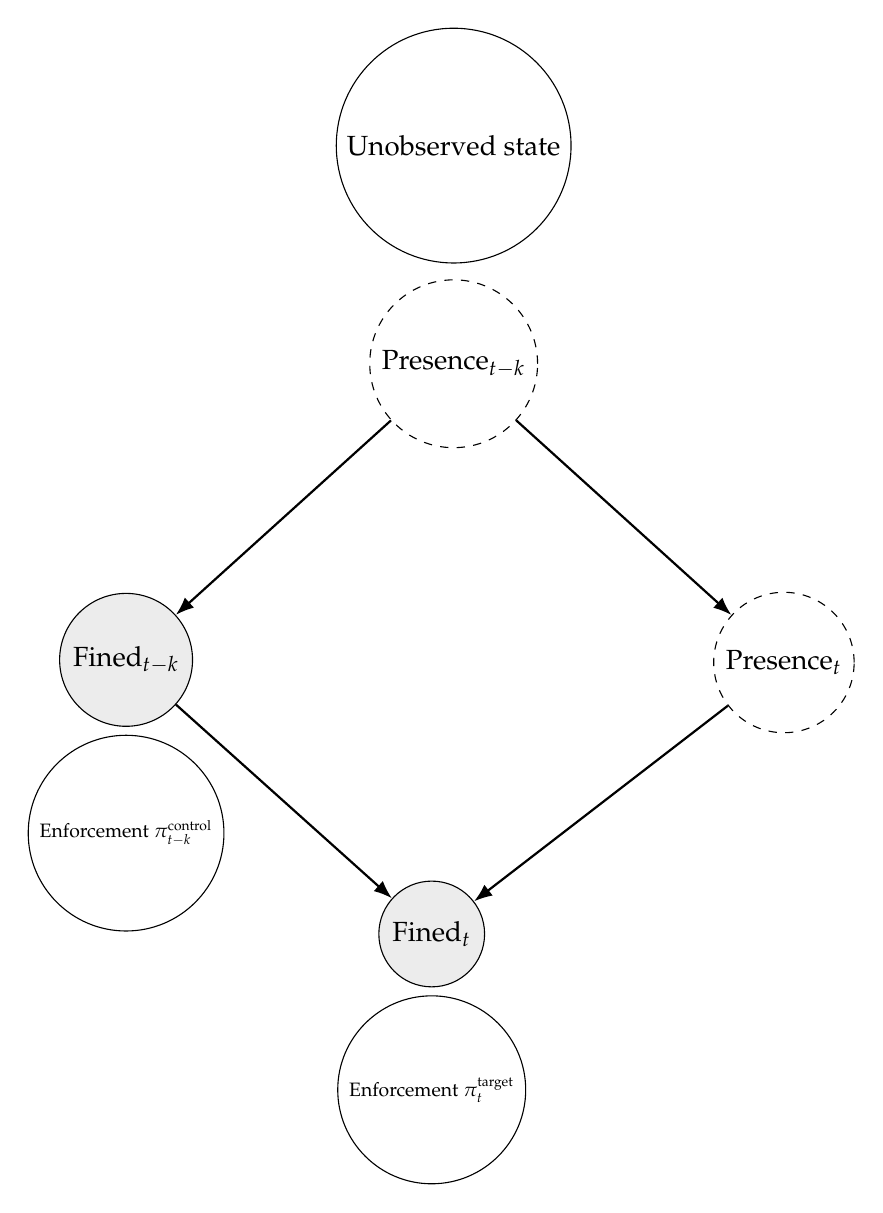
\begin{tikzpicture}[
  node distance=2.4cm and 2.8cm,
  every node/.style={draw, circle, minimum size=1.2cm, font=\normalsize},
  latent/.style={draw, circle, dashed},
  obs/.style={draw, circle, fill=gray!15},
  arrow/.style={->, >=Latex, thick}
]

% Nodes
\node[latent] (presence_tk) {Presence$_{t-k}$};
\node[obs, below left=of presence_tk] (fined_tk) {Fined$_{t-k}$};
\node[latent, below right=of presence_tk] (presence_t) {Presence$_t$};
\node[obs, below right=of fined_tk] (fined_t) {Fined$_t$};

% Arrows
\draw[arrow] (presence_tk) -- (fined_tk);
\draw[arrow] (presence_tk) -- (presence_t);
\draw[arrow] (presence_t) -- (fined_t);
\draw[arrow] (fined_tk) -- (fined_t);

% Labels
\node[align=center, above=0.2cm of presence_tk] {Unobserved state};
\node[align=center, below=0.1cm of fined_tk] {\scriptsize Enforcement $\pi^{\text{control}}_{t-k}$};
\node[align=center, below=0.1cm of fined_t] {\scriptsize Enforcement $\pi^{\text{target}}_t$};

\end{tikzpicture}
}
\caption{Directed acyclic graph showing how presence and enforcement determine fine observables. Conditioning on Fined$_{t-k}=1$ introduces selection on Presence$_{t-k}$.}
\end{figure}

\clearpage
\fi 

\iffalse
\begin{figure}[h!]
    \centering
    \caption{Illustrating Polygon Validation} \label{fig:muni_1303536_invalid_example1}
    \subfloat[All CARs in Municipality]{\includegraphics[scale=.3]{output/muni_1303536_invalid_example1.pdf}} \\
    \subfloat[Only invalid CARs]{\includegraphics[scale=.3]{output/muni_1303536_invalid_example2.pdf}} \\
    \subfloat[Validated CARs]{\includegraphics[scale=.3]{output/muni_1303536_invalid_example3.pdf}}
    \justify
    {{\it \small Notes:} \footnotesize The figure illustrates how invalid polygons are validated for municipality Presidente Figueiredo (IBGE code 1303536). Panel A presents a snapshot of all of the demarcated CARs in the municipality in 2023. Yellow indicates the CAR is valid while blue indicates the opposite. Panel B only presents the invalid polygons. Panel C presents the same CARs as in Panel B, now with validated polygons.} 
\end{figure}

\pagebreak
\begin{landscape}
\begin{figure}[h!]
    \centering
    \caption{Computing CAR Intersection over Indigenous Lands} \label{fig:muni_1303536_indigenous_example1}
    \subfloat[All CARs]{\includegraphics[scale=.35]{output/muni_1303536_indigenous_example1.pdf}} \qquad
    \subfloat[Union of CARs]{\includegraphics[scale=.35]{output/muni_1303536_indigenous_example2.pdf}} \\
    \subfloat[Overlay Indigenous Land]{\includegraphics[scale=.35]{output/muni_1303536_indigenous_example3.pdf}} \qquad
    \subfloat[Area of Intersection]{\includegraphics[scale=.35]{output/muni_1303536_indigenous_example4.pdf}}
    \justify
    {{\it \small Notes:} \footnotesize The figure illustrates how the area of intersection between the total claimed land and indigenous land is computed within a in municipality-year. The municipality in this example is Presidente Figueiredo (IBGE code 1303536). Panel A presents a snapshot of all of the demarcated CARs in the municipality. Panel B illustrates the union of all of the CAR areas. Panel C overlays indigenous lands. Panel D illustrates the areas of intersection between indigenous and demarcated CARs within the municipality.}
\end{figure}
\end{landscape}
 
\pagebreak

\begin{figure}[h!]
    \centering
    \caption{Cancelled CAR Intersections with other CARs I} \label{fig:muni_1200013_cancelled_overlap_example1}
    \subfloat[May-2014]{\includegraphics[scale=.25]{output/muni_1200013_cancelled_overlap_example1.pdf}} \\
    \subfloat[Aug-014]{\includegraphics[scale=.25]{output/muni_1200013_cancelled_overlap_example2.pdf}} \\
    \subfloat[Intersection]{\includegraphics[scale=.25]{output/muni_1200013_cancelled_overlap_example3.pdf}} \\
    \subfloat[Administrative Outcome]{\includegraphics[scale=.25]{output/muni_1200013_cancelled_overlap_example4.pdf}} 
    \justify
    {{\it \small Notes:} \footnotesize The figure illustrates the time-line of CAR claims for several properties in Acrelândia (IBGE code 1200013). 
    Panel A and B present point in time snap-snots of the CAR claims in the area. Panel C highlights the intersection between the claims. Panel 4 highlights that the original CAR in Panel A was ultimately cancelled while the second CAR is currently marked as "Active". The CAR IDS in this figures are :  "AC-1200013-7F9077EED34645E382BEB48DACF66206","AC-1200013-47340A0E7BFD43D999869111D3C47A6B"}
\end{figure}

\pagebreak

\begin{figure}[h!]
    \centering
    \caption{Cancelled CAR Intersections with other CARs II} \label{fig:muni_1200013_cancelled_overlap_example5}
    \subfloat[Feb-2015]{\includegraphics[scale=.25]{output/muni_1200013_cancelled_overlap_example5.pdf}} \\
    \subfloat[April-2016]{\includegraphics[scale=.25]{output/muni_1200013_cancelled_overlap_example6.pdf}} \\
    \subfloat[Jul-2018]{\includegraphics[scale=.25]{output/muni_1200013_cancelled_overlap_example7.pdf}}
 
    \justify
    {{\it \small Notes:} \footnotesize The figure continues the time-line from Figure \ref{fig:muni_1200013_cancelled_overlap_example1} of CAR claims for several properties in Acrelândia (IBGE code 1200013). 
    All panels present point in time snap-snots of the CAR claims in the area. Panel A shows that an additional---currently "Pending"---CAR is claimed over the now-cancelled original CAR.  Panel B shows that a far larger, currently "Active" CAR is claimed, which intersects with all previous claims. Panel C shows a final CAR, filled in red and also currently "Cancelled", is added in 2018.
    The additional CAR ID suffixes in this figure are:   "3FA22235433E4725969D1C3AEF755777", "78B561B83CBA4F0AB0A2AF4563D617F5", "C9AA224F678844A389563238E0DAB987"}
\end{figure}

\begin{figure}[h!]
    \centering
    \caption{Cancelled CAR Intersections with other CARs II} \label{fig:muni_1200013_cancelled_overlap_example5}
      \subfloat[Feb-2015]{\includegraphics[scale=.8]{output/algo_example.pdf}} 
    \justify
    {{\it \small Notes:} \footnotesize The figure continues the time-line from Figure \ref{fig:muni_1200013_cancelled_overlap_example1} of CAR claims for several properties in Acrelândia (IBGE code 1200013). 
    All panels present point in time snap-snots of the CAR claims in the area. Panel A shows that an additional---currently "Pending"---CAR is claimed over the now-cancelled original CAR.  Panel B shows that a far larger, currently "Active" CAR is claimed, which intersects with all previous claims. Panel C shows a final CAR, filled in red and also currently "Cancelled", is added in 2018.
    The additional CAR ID suffixes in this figure are:   "3FA22235433E4725969D1C3AEF755777", "78B561B83CBA4F0AB0A2AF4563D617F5", "C9AA224F678844A389563238E0DAB987"}
\end{figure}



\clearpage

\begin{figure}[h!]
    \centering
    \caption{Cancelled CAR Intersections with other CARs II} \label{fig:muni_1200013_cancelled_overlap_example5}
    \subfloat[Feb-2015]{\includegraphics[scale=.6]{output/i_contains_minus_i.pdf}}  
     \subfloat[Feb-2015]{\includegraphics[scale=.6]{output/i_contains_minus_i.pdf}} 
    \justify
    {{\it \small Notes:} \footnotesize The figure continues the time-line from Figure \ref{fig:muni_1200013_cancelled_overlap_example1} of CAR claims for several properties in Acrelândia (IBGE code 1200013). 
    All panels present point in time snap-snots of the CAR claims in the area. Panel A shows that an additional---currently "Pending"---CAR is claimed over the now-cancelled original CAR.  Panel B shows that a far larger, currently "Active" CAR is claimed, which intersects with all previous claims. Panel C shows a final CAR, filled in red and also currently "Cancelled", is added in 2018.
    The additional CAR ID suffixes in this figure are:   "3FA22235433E4725969D1C3AEF755777", "78B561B83CBA4F0AB0A2AF4563D617F5", "C9AA224F678844A389563238E0DAB987"}
\end{figure}



\clearpage

 \begin{figure}[h!]
    \centering
    \caption{Cancelled CARs by Municipality} \label{fig:cancelled_cars_number_by_muni_map}
    \includegraphics[scale=.35]{output/cancelled_cars_number_by_muni_map.pdf}
    %\subfloat[Percentage of CARs cancelled]{\includegraphics[scale=.235]{output/cancelled_cars_perc_by_muni_map.pdf}  
    %\subfloat[Percentage of CARs cancelled]{\includegraphics[scale=.225]{output/cancelled_cars_rel_by_muni.pdf} 
    \vspace{2mm}
    \justify
   { {\it \small Notes:} \footnotesize The figure presents the number of cancelled CARs per municipality.
    }
\end{figure}

 \begin{figure}[h!]
    \centering
    \caption{Cancelled CARs by Municipality} \label{fig:cancelled_cars_perc_by_muni_map}
    \includegraphics[scale=.35]{output/cancelled_cars_perc_by_muni_map.pdf}
    %\subfloat[Percentage of CARs cancelled]{\includegraphics[scale=.235]{output/cancelled_cars_perc_by_muni_map.pdf}  
    %\subfloat[Percentage of CARs cancelled]{\includegraphics[scale=.225]{output/cancelled_cars_rel_by_muni.pdf} 
    \vspace{2mm}
    \justify
  {  {\it \small Notes:} \footnotesize The figure presents the number of cancelled over the total CARs per municipality.
    }
\end{figure}

\begin{landscape}
     \begin{figure}[h!]
    \centering
    \caption{Cancelled CARs by Municipality} \label{fig:cancelled_cars_rel_by_muni}
    \includegraphics[scale=.55]{output/cancelled_cars_rel_by_muni.pdf}
    %\subfloat[Percentage of CARs cancelled]{\includegraphics[scale=.235]{output/cancelled_cars_perc_by_muni_map.pdf}  
    %\subfloat[Percentage of CARs cancelled]{\includegraphics[scale=.225]{output/cancelled_cars_rel_by_muni.pdf} 
    \vspace{2mm}
    \justify
   { {\it \small Notes:} \footnotesize The figure presents the number of total and cancelled CARs per labelled municipality. The size of the municipality label corresponds to the share of cancelled CARs in that municipality. The dotted line traces the 10\% mark as municipality size increases. 
    }
\end{figure}
\end{landscape}

\begin{landscape}
    \begin{figure}[h!]
    \centering
    \caption{Union of CARs by Municipality - Year} \label{fig:car_union_area_all_map}
    \includegraphics[scale=.45]{output/car_union_area_all_map.pdf}
    \vspace{2mm}
    \justify
  {  {\it \small Notes:} \footnotesize The figure presents the total area of land per municipality-year that is claimed by at least one CAR. We take the union of all CARs to avoid double counting intersections. All areas are in square kilometers. 
    }
\end{figure}    
\end{landscape}

\begin{landscape}
    \begin{figure}[h!]
    \centering
    \caption{Intersection of Union of CARs and Conservation land by Municipality - Year} \label{fig:car_area_intersect_conserve_all_map}
    \includegraphics[scale=.45]{output/car_area_intersect_conserve_over_car_map.pdf}
    \vspace{2mm}
    \justify
    {{\it \small Notes:} \footnotesize The figure presents the share of claimed land that intersects with conservation land. That is, each unit corresponds to the area of intersection between the Union of CARs (total area of land per municipality-year that is claimed by at least one CAR) and intersects with protected conservation land over the area of the Union of CARs. We take the union of all CARs to avoid double counting intersections. 
    }
\end{figure}
\end{landscape}

\begin{landscape}
\begin{figure}[h!]
    \centering
    \caption{Intersection of Union of CARs and Indigenous land by Municipality - Year} \label{fig:car_area_intersect_indi_all_map}
    \includegraphics[scale=.45]{output/car_area_intersect_indi_over_car_map.pdf}
    \vspace{2mm}
    \justify
   { {\it \small Notes:} \footnotesize The figure presents the share of claimed land that intersects with indigenous land. That is, each unit corresponds to the area of intersection between the Union of CARs (total area of land per municipality-year that is claimed by at least one CAR) and intersects with protected Indigenous land over the area of the Union of CARs. We take the union of all CARs to avoid double counting intersections. 
    }
\end{figure}
\end{landscape}

\begin{landscape}
    \begin{figure}[h!]
    \centering
    \caption{Intersection of Union of CARs and Forested land by Municipality - Year} \label{fig:car_area_intersect_conserve_all_map}
    \includegraphics[scale=.45]{output/car_area_intersect_forest_over_car_map.pdf}
    \vspace{2mm}
    \justify
    {{\it \small Notes:} \footnotesize The figure presents the share of claimed land that intersects with forested land. That is, each unit corresponds to the area of intersection between the Union of CARs (total area of land per municipality-year that is claimed by at least one CAR) and intersects with protected forested land over the area of the Union of CARs. We take the union of all CARs to avoid double counting intersections. 
    }
\end{figure}
\end{landscape}



    \begin{figure}[h!]
    \centering
    \caption{Share of CAR Conflicts by Intersection Bucket - By Municipality} \label{fig:share_of_intersected_cars}
    \includegraphics[scale=.65]{output/share_of_intersected_cars.pdf}
    \vspace{2mm}
    \justify
    {{\it \small Notes:} \footnotesize The figure presents the share of CAR overlaps (or conflicts) within each municipality in a given year. Each column corresponds to an intersection bucket, indicating the range of the area of the overlap as a percentage of the area of a reference CAR. Each row corresponds to a year and is independent from the next row. For any given municipality, summing across rows equals one.     
    For example, consider a random municipality M in the upper left figure, 'CAR (0, 33]\%, 2015'. The color of municipality M corresponds to the number of unique conflicts in 2015 that fell between 0-33\% of the reference CAR's land, divided by the total number of conflicts in municipality M in 2015. Since most conflicts are fairly small, the majority of conflicts falls within the (0,33]\% bucket. 
    Notice that there may be multiple conflicts per CAR and that we only consider conflicts where the reference CAR is newer than the intersecting CAR, in order to avoid double counting. For example, if CARs A, B and C appeared in this order, all in 2015 and have overlapping claims. We would include the intersection of: B over A as a share of B, C over A as a share of C, and C over B as a share of C. 
    }
\end{figure}




\begin{figure}[h!]
    \centering
    \caption{Number of Overlaps Conditional on Reference CAR Outcome} \label{fig:n_overlaps_conditional_on_pending}
    \subfloat[Active]{}{\includegraphics[scale=.2]{output/n_overlaps_conditional_on_active.pdf}}
    \subfloat[Cancelled]{}{\includegraphics[scale=.2]{output/n_overlaps_conditional_on_cancelled.pdf}}
    \subfloat[Pending]{}{    \includegraphics[scale=.2]{output/n_overlaps_conditional_on_pending.pdf}}
    \vspace{2mm}
    \justify
    {{\it \small Notes:} \footnotesize The figure presents the number of cancelled CAR intersections over the number of total number of CAR intersections per intersection bucket, year. An intersection bucket is the share of land from a reference CAR which overlaps with an existing CAR. For example, suppose CAR A is intersected by two older CARs: B and C at 5\% and 15\% of its land. We would then count CAR A in both the 0-10\% bucket and 10-20\% bucket, dividing it by the total number of intersections present, in this case 2.

    }
\end{figure}

\begin{landscape}
    \begin{figure}[h!]
    \centering
    \caption{Proportion of Intersections Conditional on Reference CAR being cancelled: Intersection Bucket - Year} \label{fig:intersection_buckets_cancelled_over_total}
    \includegraphics[scale=.45]{output/intersection_buckets_cancelled_over_total.pdf}
    \vspace{2mm}
    \justify
    {{\it \small Notes:} \footnotesize The figure presents number of cancelled CAR intersections over the number of total number of CAR intersections per intersection bucket, year. An intersection bucket is the share of land from a reference CAR which overlaps with an existing CAR. For example, suppose CAR A is intersected by two older CARs: B and C at 5\% and 15\% of its land. We would then count CAR A in both the 0-10\% bucket and 10-20\% bucket, dividing it by the total number of intersections present, in this case 2.

    }
\end{figure}
\end{landscape}


%%%%%%% Number of CARs
\begin{landscape}
    \begin{table}[ht]
    \centering
    \caption{CARs and Intersections}\label{tab:number_of_cars}
    \begin{tabular}{rcccccc}
      \toprule
      &(1)&(2)&(3)&(4)&(5)&(6)\\
      Year & \multicolumn{6}{c}{Number of CARs}    \vspace{2mm} \\
    \cline{2-7} \vspace{2mm}
       &  & With intersection & Both AT & Neither CA & Target is CA & Reference is CA \\ 
       \hline 
2014 & 56,130 & 28,999 & 21,225 & 26,289 & 2,719 & 3,097 \\ 
  2015 & 208,075 & 104,553 & 39,086 & 96,323 & 8,150 & 11,081 \\ 
  2016 & 129,803 & 92,303 & 48,281 & 86,669 & 10,830 & 4,850 \\ 
  2017 & 54,215 & 37,641 & 19,976 & 35,800 & 5,096 & 1,310 \\ 
  2018 & 66,844 & 48,057 & 26,299 & 43,823 & 6,478 & 3,767 \\ 
  2019 & 68,843 & 49,588 & 33,452 & 47,610 & 6,610 & 1,219 \\ 
  2020 & 73,198 & 51,955 & 33,865 & 50,205 & 6,433 & 1,077 \\ 
  2021 & 82,524 & 63,865 & 41,949 & 62,400 & 7,482 & 927 \\ 
  2022 & 62,093 & 49,787 & 36,256 & 48,970 & 5,681 & 346 \\ 
  2023 & 27 & 25 &  &  & 9 & 27 \\ 
       \bottomrule
    \end{tabular}
    \justify{
\footnotesize \textit{Notes:} The table presents summary statistics using number of CARs in the Amazon biome as the unit of measurement. Column (1) presents the total number of CARs according to their year of registration. Call these reference CARs. Columns (2)-(6) present the number of  reference CARs which have some type of an intersection with intersecting (target) CAR. In this table, target CARs always have a registration year equal to or less than the reference CAR. Column (2) presents the number of reference CARs which have at least one intersection. Column (3) presents the number of reference CARs which are active (Status=="AT") and which intersect with active target CARs. Column (4) presents the number of reference CARs which are not cancelled (Status!="CA") and which intersect with target CARs that are also not cancelled.  Column (5) presents the number of reference CARs which intersect with cancelled target CARs. Column (6) presents the number of reference CARs which are cancelled.
    }
\end{table}
\end{landscape}


\begin{table}[ht]
\centering
\caption{Probability of a CAR being born into conflict, by the largest conflict percentage, conditional on current CAR status.}\label{tab:prob_of_beingborn_into_conflict}
\begin{tabular}{rrrrr}
  \hline
$\leq$Bucket & CA & AT & PE & SU \\ 
  \hline
33 & 31 & 37 & 40 & 36 \\ 
  66 & 3 & 4 & 4 & 3 \\ 
  99$.\bar{9}$ & 10 & 7 & 6 & 6 \\ 
  100 & 29 & 21 & 16 & 31 \\ 
   \hline
\end{tabular}
 \justify{
\footnotesize \textit{Notes:} The table presents the conditional probability of a CAR being created with a conflict, conditional on it's current status. For instance, column "CA" considers all CARs with status = "CA" and identifies whether each CAR had an intersection from the moment it was created. For the CARs with at least one intersection, we compute the largest intersection in terms of the CAR's area. If multiple intersection exist, we only consider the largest one. We then divide by the total number of CARs with status = "CA". Notice, a CAR can be completely covered by its neighbors from the moment it is created, but still fall within the smallest bucket (e.g. $\leq33\%$, if the largest intersection is less than the bucket's threshold of 33\%.

}
\end{table}


\begin{table}[ht]
\centering
\caption{Joint Distribution of Reference and Target CAR Intersections}
\begin{tabular}{rlrrrrrr}
  \hline
 & Reference Status & NA & AT & CA & PE & RE & SU \\ 
  \hline
1 & AT & 25.60 & 28.10 & 2.30 & 9.40 & 0.00 & 0.70 \\ 
  2 & CA & 1.30 & 1.60 & 0.70 & 0.80 & 0.00 & 0.10 \\ 
  3 & PE & 9.80 & 3.90 & 0.90 & 12.00 & 0.00 & 0.30 \\ 
  4 & RE & 0.00 & 0.00 & 0.00 & 0.00 & 0.00 & 0.00 \\ 
  5 & SU & 0.90 & 0.90 & 0.20 & 0.20 & 0.00 & 0.40 \\ 
   \hline
\end{tabular}
 \justify{
\footnotesize \textit{Notes:} The table presents the joint distribution of reference and target CARs by their status.

}
\end{table}

\pagebreak


%     \subfloat[Percentage of CARs cancelled]{\includegraphics[scale=.025]{output/cancelled_cars_rel_by_muni.pdf} 
\fi 


\section*{Overview}
This section details the procedure used to construct the enforcement intensity estimators, as implemented in the provided \texttt{R} script. The process involves two primary stages. First, we establish a link between satellite-detected deforestation warnings and subsequently issued environmental fines using a spatio-temporal matching algorithm. Second, using these matched pairs, we compute both a naive enforcement rate and a robust rate that adjusts for satellite observation censorship due to cloud cover, as discussed in the paper.

\section*{Stage 1: Spatio-Temporal Matching of Fines to Warnings}
To measure enforcement, we first identify which deforestation warnings plausibly triggered a corresponding environmental fine. A match is established if a fine is issued within a proximate spatial and temporal window following a warning.

\subsection*{Spatial Matching Criterion}
The spatial link is created by generating a circular area of influence around each deforestation warning polygon. The provided \texttt{R} code implements this by first transforming the coordinate reference system to a metric projection (EPSG:3857) to allow for distance-based calculations.

For each warning, a circular buffer is created. The radius ($r$) of this buffer is determined by a pre-defined area ($A$), ensuring that each buffer represents a constant search area. The analysis is conducted for multiple buffer areas (e.g., 0.5, 1.0, and 2.0 hectares). The radius is calculated as:
$$
r = \sqrt{\frac{A}{\pi}}
$$
A fine, represented by its geographic point coordinates, is considered a spatial match if it falls within the boundary of a warning's circular buffer.

\subsection*{Temporal Matching Criterion}
A spatially matched fine is only considered a valid enforcement action if its date of issuance occurs within a pre-defined time window following the warning's observation date. The script defines this window as being between the day of the warning and six months after:
$$
t_{warning} \leqslant t_{fine} \leqslant t_{warning} + 6 \text{ months}
$$
The total count of fines satisfying both criteria in a given region $g$ (e.g., control or target area) and time period $t$ is denoted as $F_{g,t}$.

\section*{Stage 2: Construction of Enforcement Estimators}

\subsection*{The Naive Enforcement Estimator}
The naive estimator of enforcement intensity, $\hat{\pi}_{g,t}$, is the simple ratio of the number of matched fines ($F_{g,t}$) to the total number of observed warnings ($W_{g,t}$) in a given region and time period.
\begin{equation}
\hat{\pi}_{g,t} = \frac{F_{g,t}}{W_{g,t}}
\end{equation}
This estimator is biased when $W_{g,t}$ is censored by factors such as cloud cover, as it underestimates the true extent of detectable illegal activity.

\subsection*{The Cloud-Adjusted Enforcement Estimator}
To correct for observational censorship, we construct a cloud-adjusted estimator, $\hat{\pi}_{g,t}^{cloud}$, following the logic outlined in the paper. This procedure relies on the assumption that the rate of illegal activity is uniform across both clear and cloud-covered areas within a region.

\paragraph{Step 1: Calculate Visible Area Fraction ($v_{g,t}$)}
For each region $g$ and time period $t$, the program calculates the fraction of the total area that is observable (i.e., cloud-free). This is done by spatially intersecting the region's polygon with shapefiles of cloud-free areas. The visible fraction, $v_{g,t}$, is the ratio of the resulting clear area to the total regional area:
$$
v_{g,t} = \frac{\text{Area}(g \cap \text{ClearSpot}_t)}{\text{Area}(g)}
$$


\paragraph{Step 2: Compute Cloud-Adjusted Enforcement Rate ($\hat{\pi}_{g,t}^{cloud}$)}
Finally, the cloud-adjusted enforcement rate is computed by dividing the number of matched fines by the estimated total (not just observed) number of warnings.
\begin{equation}
\hat{\pi}_{g,t}^{cloud} = \frac{F_{g,t}}{\hat{W}^{total}_{g,t}} = \frac{F_{g,t}}{(W_{g,t} / v_{g,t})}
\end{equation}

\end{appendices}

\end{document}

Coding Objectives: 

- For each municipality, year: 

    - Compute total area
    
    - Take union of CARs and compute : 
        - area with cancelled CARs
            - by it self
            - intersects with indigenous land
            - intersects with forested land (three types)
            - intersects with conservation land
            
        - area without cancelled CARs
            - by it self
            - intersects with indigenous land
            - intersects with forested land (three types)
            - intersects with conservation land
        
- For each CARID in a municipality, year:

    - compute it's area
    
    - compute it's intersection area with:
        - convervation
        - forrested
        - indigenous lands
        - each neighboring CAR 


Output objectives: 

    - Visual example of process for computing areas 

    - Visual example of process for conflicts 
        - looking at cancelled CARs 
        - looking at normal CARs


    - Summary statistics A
        - Total computed area for all municipalities
        - Total computed area for all CARs
        - Total computed area for all cancelled CARs
        - Total computed area for intersection with conservation area
        - Total computed area for intersection with forested area
        - Total computed area for intersection with indigenous area
        - Total computed area in terms of CAR over-laps  
        - Total computed area in terms of CAR over-laps without cancelled CARs
        - Total computed area of complete CAR over-laps
        - Fraction of CARs with conflict
        - Avg percentage of CAR land that is in conflict


  
	a gente tem o \%overlap por municipio, \%area cancelada por municipio, \%CARs irregulares ou cancelados


1. pra cada i (CAR ID) ver se tem algum overlap com algum outro CAR ID j. Começa com todos os anos.
2. se i tem 100% de overlap com um j e o ano de j veio depois do ano de i, a gente usa i ate o ano prior to ano de j, depois so j.
3. se i tem 100% de overlap com um j e o ano de j é menor ou igual a i, use so j
4. se i tem 100% de overlap com um j e <100% de overlap com um k, aplica a mesma regra acima, depois compara j com k (p determinar o overlap entre os dois) como se i nao tivesse existido
----
5. se i e j tem overlap <100%: a gente usa os dois separados, mas dai a questao eh a area do overlap